% !TEX program = xelatex
% =====================================================================
%  BÁO CÁO BÀI TẬP LỚN — IT4788 PHÁT TRIỂN ỨNG DỤNG ĐA NỀN TẢNG
%  Đề tài: Xây dựng ứng dụng di động đa nền tảng “Đi chợ tiện lợi”
%  Biên dịch: latexmk -xelatex main.tex   (xem README.md)
% =====================================================================
\documentclass[a4paper,12pt,oneside]{report}
% =====================================================================
%  preamble.tex — Cấu hình định dạng báo cáo IT4788
%  Bám theo mẫu dsds.docx: A4, lề trên/dưới/phải 2 cm, lề trái 3 cm,
%  thân văn bản 13 pt, tiêu đề Arial (chương 17 pt, mục 15 pt, mục con 14 pt).
%  Biên dịch bằng XeLaTeX (hoặc LuaLaTeX).
% =====================================================================

% ---------- Bố cục trang ----------------------------------------------
\usepackage[a4paper,top=2cm,bottom=2cm,left=3cm,right=2cm,
            headheight=16pt,headsep=0.35cm,footskip=0.9cm]{geometry}

% ---------- Phông chữ và ngôn ngữ ------------------------------------
\usepackage{fontspec}
\usepackage{polyglossia}
\setdefaultlanguage{vietnamese}
\setotherlanguage{english}

% Ưu tiên phông của mẫu Word; tự chuyển sang phông tương đương khi máy
% biên dịch (ví dụ Overleaf) không cài Times New Roman / Arial.
\IfFontExistsTF{Times New Roman}
  {\setmainfont{Times New Roman}}
  {\setmainfont{TeX Gyre Termes}}
\IfFontExistsTF{Arial}
  {\newfontfamily\headingfont{Arial}\setsansfont{Arial}}
  {\newfontfamily\headingfont{TeX Gyre Heros}\setsansfont{TeX Gyre Heros}}
\IfFontExistsTF{JetBrains Mono}
  {\setmonofont{JetBrains Mono}[Scale=0.9]}
  {\IfFontExistsTF{TeX Gyre Cursor}
     {\setmonofont{TeX Gyre Cursor}[Scale=0.9]}
     {\setmonofont{FreeMono}[Scale=0.9]}}

% Cỡ chữ thân bài 13 pt (lớp report chuẩn không có sẵn cỡ này)
\makeatletter
\renewcommand\normalsize{%
  \@setfontsize\normalsize{13pt}{15.6pt}%
  \abovedisplayskip 10\p@ \@plus3\p@ \@minus6\p@
  \abovedisplayshortskip \z@ \@plus3\p@
  \belowdisplayshortskip 6\p@ \@plus3\p@ \@minus3\p@
  \belowdisplayskip \abovedisplayskip
  \let\@listi\@listI}
\renewcommand\small{\@setfontsize\small{12pt}{14.4pt}}
\renewcommand\footnotesize{\@setfontsize\footnotesize{11pt}{13.2pt}}
\renewcommand\scriptsize{\@setfontsize\scriptsize{9pt}{10.8pt}}
\renewcommand\large{\@setfontsize\large{14pt}{16.8pt}}
\renewcommand\Large{\@setfontsize\Large{15pt}{18pt}}
\renewcommand\LARGE{\@setfontsize\LARGE{17pt}{20.4pt}}
\renewcommand\huge{\@setfontsize\huge{20pt}{24pt}}
\renewcommand\Huge{\@setfontsize\Huge{24pt}{28.8pt}}
\makeatother
\normalsize

% ---------- Gói tiện ích ----------------------------------------------
\usepackage{etoolbox}
\usepackage{setspace}
\usepackage{indentfirst}
\usepackage{graphicx}
\usepackage[table]{xcolor}
\usepackage{array}
\usepackage{longtable}
\usepackage{tabularx}
\usepackage{multirow}
\usepackage{makecell}
\usepackage{booktabs}
\usepackage{float}
\usepackage{pdflscape}
\usepackage{caption}
\usepackage{enumitem}
\usepackage{amsmath}
\usepackage{unicode-math}
% Phông toán cùng phong cách Times; nếu không có thì dùng Latin Modern Math mặc định
\IfFontExistsTF{TeX Gyre Termes Math}
  {\setmathfont{TeX Gyre Termes Math}}
  {\IfFontExistsTF{STIX Two Math}
     {\setmathfont{STIX Two Math}}
     {\IfFontExistsTF{Cambria Math}
        {\setmathfont{Cambria Math}}
        {\setmathfont{Latin Modern Math}}}}
\usepackage{fancyvrb}
\usepackage{tikz}
\usepackage{titlesec}
\usepackage{titletoc}
\usepackage{fancyhdr}
\usepackage{csquotes}
\DeclareQuoteStyle{vietnamese}
  {\textquotedblleft}
  {\textquotedblright}
  {\textquoteleft}
  {\textquoteright}
\usepackage[unicode,hidelinks,bookmarksnumbered]{hyperref}

% Cho phép ngắt dòng tại dấu gạch nối trong \url, \path
\appto\UrlBreaks{\do\-}

\graphicspath{{figures/}{figures/diagrams/}}

% ---------- Giãn dòng, đoạn văn ----------------------------------------
\setstretch{1.3}
\setlength{\parindent}{1cm}
\setlength{\parskip}{2pt plus 1pt}
\emergencystretch=2em
\widowpenalty=10000
\clubpenalty=10000

% Bảng dùng giãn dòng đơn để gọn
\AtBeginEnvironment{tabular}{\setstretch{1.05}}
\AtBeginEnvironment{tabularx}{\setstretch{1.05}}
\AtBeginEnvironment{longtable}{\setstretch{1.05}}
\renewcommand{\arraystretch}{1.2}

% ---------- Màu sắc ----------------------------------------------------
\definecolor{hustred}{HTML}{B5121B}
\definecolor{headerbg}{HTML}{DCE6F2}
\definecolor{subheaderbg}{HTML}{F2F5FA}
\definecolor{rulegray}{HTML}{7F7F7F}
\definecolor{codebg}{HTML}{F7F7F7}

% ---------- Nhãn tiếng Việt --------------------------------------------
\gappto\captionsvietnamese{%
  \renewcommand{\contentsname}{MỤC LỤC}%
  \renewcommand{\listfigurename}{DANH MỤC HÌNH VẼ}%
  \renewcommand{\listtablename}{DANH MỤC BẢNG BIỂU}%
  \renewcommand{\figurename}{Hình}%
  \renewcommand{\tablename}{Bảng}%
  \renewcommand{\chaptername}{Chương}%
  \renewcommand{\appendixname}{Phụ lục}%
  \renewcommand{\bibname}{TÀI LIỆU THAM KHẢO}%
}

% ---------- Tiêu đề chương, mục ---------------------------------------
\setcounter{secnumdepth}{4}
\setcounter{tocdepth}{3}
\renewcommand{\thesubsubsection}{\thesubsection.\arabic{subsubsection}}

\titleformat{\chapter}[block]
  {\headingfont\bfseries\fontsize{17pt}{21pt}\selectfont\centering}
  {CHƯƠNG \thechapter.}{0.4em}{}
\titleformat{name=\chapter,numberless}[block]
  {\headingfont\bfseries\fontsize{17pt}{21pt}\selectfont\centering}
  {}{0pt}{}
\titlespacing*{\chapter}{0pt}{0pt}{24pt}

\titleformat{\section}
  {\headingfont\bfseries\fontsize{15pt}{18pt}\selectfont}
  {\thesection.}{0.5em}{}
\titlespacing*{\section}{0pt}{18pt}{10pt}

\titleformat{\subsection}
  {\headingfont\bfseries\fontsize{14pt}{17pt}\selectfont}
  {\thesubsection.}{0.5em}{}
\titlespacing*{\subsection}{0pt}{12pt}{8pt}

\titleformat{\subsubsection}
  {\headingfont\bfseries\fontsize{13pt}{16pt}\selectfont}
  {\thesubsubsection.}{0.5em}{}
\titlespacing*{\subsubsection}{0pt}{10pt}{6pt}

\titleformat{\paragraph}[runin]
  {\headingfont\bfseries\itshape}{}{0pt}{}[.]
\titlespacing*{\paragraph}{\parindent}{6pt}{0.5em}

% ---------- Mục lục, danh mục hình/bảng ----------------------------------
\titlecontents{chapter}[0pt]
  {\addvspace{6pt}\bfseries}
  {CHƯƠNG \thecontentslabel.\ }
  {}
  {\titlerule*[0.6pc]{.}\contentspage}
\titlecontents{section}[1.2em]
  {\addvspace{1pt}}
  {\contentslabel[\thecontentslabel.]{2.4em}}
  {}
  {\titlerule*[0.6pc]{.}\contentspage}
\titlecontents{subsection}[3.6em]
  {\addvspace{0pt}\itshape}
  {\contentslabel[\thecontentslabel.]{3.0em}}
  {}
  {\titlerule*[0.6pc]{.}\contentspage}
\titlecontents{figure}[0pt]
  {\addvspace{1pt}}
  {Hình \thecontentslabel.\ }
  {}
  {\titlerule*[0.6pc]{.}\contentspage}
\titlecontents{table}[0pt]
  {\addvspace{1pt}}
  {Bảng \thecontentslabel.\ }
  {}
  {\titlerule*[0.6pc]{.}\contentspage}

% ---------- Chú thích hình, bảng ---------------------------------------
\captionsetup{font={small},labelfont=bf,labelsep=period,
              justification=centering,singlelinecheck=true}
\captionsetup[figure]{skip=6pt}
\captionsetup[table]{position=top,skip=4pt}
\captionsetup[longtable]{position=top}

% ---------- Đầu trang, chân trang --------------------------------------
\newcommand{\coursename}{IT4788 – Phát triển ứng dụng đa nền tảng}
\newcommand{\projectname}{Ứng dụng “Đi chợ tiện lợi”}
\newcommand{\groupname}{Nhóm 7}

\fancypagestyle{main}{%
  \fancyhf{}%
  \fancyhead[L]{\small\itshape\coursename}%
  \fancyhead[R]{\small\itshape\projectname}%
  \fancyfoot[L]{\small\groupname}%
  \fancyfoot[R]{\small\thepage}%
  \renewcommand{\headrulewidth}{0.4pt}%
  \renewcommand{\footrulewidth}{0.4pt}}
\fancypagestyle{plain}{%
  \fancyhf{}%
  \fancyhead[L]{\small\itshape\coursename}%
  \fancyhead[R]{\small\itshape\projectname}%
  \fancyfoot[L]{\small\groupname}%
  \fancyfoot[R]{\small\thepage}%
  \renewcommand{\headrulewidth}{0.4pt}%
  \renewcommand{\footrulewidth}{0.4pt}}

% ---------- Danh sách (hạn chế dùng, chỉ khi thật cần) ------------------
\setlist{itemsep=2pt,topsep=4pt,parsep=0pt,leftmargin=1.6em}

% ---------- Mã nguồn ---------------------------------------------------
% fancyvrb hiển thị đúng tiếng Việt có dấu với XeLaTeX (listings làm đảo dấu)
\fvset{fontsize=\footnotesize,frame=single,framesep=5pt,rulecolor=\color{rulegray},
       numbers=left,numbersep=5pt,xleftmargin=16pt,baselinestretch=1}
\DeclareCaptionType[fileext=lol]{code}[Mã nguồn][Danh mục mã nguồn]
\captionsetup[code]{skip=4pt}
\newcommand{\codecaption}[2]{%
  \noindent\begin{minipage}{\textwidth}
    \captionsetup{type=code}%
    \caption{#1}\label{#2}%
  \end{minipage}\par}

% ---------- Lệnh tiện ích dùng trong báo cáo ----------------------------
% Chèn sơ đồ PlantUML đã sinh ra ảnh PNG
% \diagram[độ rộng]{tên tệp}{chú thích}{nhãn}
\newcommand{\diagram}[4][\textwidth]{%
  \begin{figure}[H]
    \centering
    \includegraphics[width=#1,height=0.78\textheight,keepaspectratio]{#2}
    \caption{#3}\label{#4}
  \end{figure}}

% Ô tiêu đề bảng
\newcommand{\hd}[1]{\cellcolor{headerbg}\textbf{#1}}
\newcommand{\hs}[1]{\cellcolor{subheaderbg}\textbf{#1}}

% Mã tham chiếu: use case, quy tắc nghiệp vụ, thông điệp, yêu cầu phi chức năng
\newcommand{\uc}[1]{\textsf{\small #1}}
\newcommand{\br}[1]{\textsf{\small #1}}
\newcommand{\msg}[1]{\textsf{\small #1}}
\newcommand{\nfr}[1]{\textsf{\small #1}}

% =====================================================================
%  ucspec.tex — Môi trường đặc tả use case và bảng dữ liệu đầu vào
%  Bố cục bám theo bảng mẫu "Đặc tả ca sử dụng" trong dsds.docx.
% =====================================================================

\newlength{\ucA}\newlength{\ucB}\newlength{\ucC}\newlength{\ucD}
\newlength{\ucBCD}\newlength{\ucCD}
\newcommand{\ucsetwidths}{%
  \setlength{\ucA}{2.55cm}\setlength{\ucB}{2.75cm}\setlength{\ucC}{2.55cm}%
  \setlength{\ucD}{\dimexpr\textwidth-8\tabcolsep-5\arrayrulewidth-\ucA-\ucB-\ucC\relax}%
  \setlength{\ucBCD}{\dimexpr\ucB+\ucC+\ucD+4\tabcolsep+2\arrayrulewidth\relax}%
  \setlength{\ucCD}{\dimexpr\ucC+\ucD+2\tabcolsep+\arrayrulewidth\relax}}

\newcolumntype{L}[1]{>{\raggedright\arraybackslash}p{#1}}
\newcolumntype{C}[1]{>{\centering\arraybackslash}p{#1}}

% \begin{ucspec}{UC01}{Đăng ký tài khoản} ... \end{ucspec}
\newenvironment{ucspec}[2]{%
  \ucsetwidths\small
  \begin{longtable}{|L{\ucA}|L{\ucB}|L{\ucC}|L{\ucD}|}
  \caption{Đặc tả use case #1 – #2}\label{tab:#1}\\
  \hline
  \hd{Mã use case} & \textbf{#1} & \hd{Tên use case} & \textbf{#2}\\ \hline
  \endfirsthead
  \multicolumn{4}{l}{\footnotesize\itshape Bảng \thetable\ (tiếp theo) – #1 – #2}\\ \hline
  \endhead
  \endfoot
  \endlastfoot
}{\end{longtable}}

% Một dòng thuộc tính: nhãn ở cột 1, nội dung trải 3 cột còn lại
\newcommand{\ucfield}[2]{%
  \hd{#1} & \multicolumn{3}{L{\ucBCD}|}{#2}\\ \hline}

% Mở đầu một luồng sự kiện (chính / thay thế / ngoại lệ)
\newcommand{\ucflow}[1]{%
  \multicolumn{4}{|l|}{\cellcolor{headerbg}\textbf{#1}}\\ \hline
  \hs{STT} & \hs{Thực hiện bởi} & \multicolumn{2}{L{\ucCD}|}{\cellcolor{subheaderbg}\textbf{Hành động}}\\ \hline}

% Một bước trong luồng sự kiện
\newcommand{\ucstep}[3]{%
  #1 & #2 & \multicolumn{2}{L{\ucCD}|}{#3}\\ \hline}

% ---------------------------------------------------------------------
% Bảng mô tả dữ liệu đầu vào của một use case
% \begin{fieldtable}{Chú thích}{nhãn} \frow{...}{...}{...}{...}{...} \end{fieldtable}
\newlength{\ftLast}
\newenvironment{fieldtable}[2]{%
  \small
  \setlength{\ftLast}{\dimexpr\textwidth-12\tabcolsep-7\arrayrulewidth-0.95cm-2.5cm-2.9cm-1.25cm-3.2cm\relax}%
  \begin{longtable}{|C{0.95cm}|L{2.5cm}|L{2.9cm}|C{1.25cm}|L{3.2cm}|L{\ftLast}|}
  \caption{#1}\label{#2}\\
  \hline
  \hd{STT} & \hd{Trường dữ liệu} & \hd{Mô tả} & \hd{Bắt buộc} & \hd{Điều kiện hợp lệ} & \hd{Ví dụ}\\ \hline
  \endfirsthead
  \multicolumn{6}{l}{\footnotesize\itshape Bảng \thetable\ (tiếp theo)}\\ \hline
  \hd{STT} & \hd{Trường dữ liệu} & \hd{Mô tả} & \hd{Bắt buộc} & \hd{Điều kiện hợp lệ} & \hd{Ví dụ}\\ \hline
  \endhead
  \endfoot
  \endlastfoot
}{\end{longtable}}
\newcounter{frowcnt}
\AtBeginEnvironment{fieldtable}{\setcounter{frowcnt}{0}}
\newcommand{\frow}[5]{%
  \stepcounter{frowcnt}\thefrowcnt & #1 & #2 & #3 & #4 & #5\\ \hline}

% ---------------------------------------------------------------------
% Bảng phân rã nghiệp vụ theo mô hình Đầu vào – Xử lý – Đầu ra
% \begin{nvtable}{Chú thích}{nhãn} \nvrow{Mã}{Nghiệp vụ}{Đầu vào}{Xử lý}{Đầu ra} \end{nvtable}
\newlength{\nvX}
\newenvironment{nvtable}[2]{%
  \small
  \setlength{\nvX}{\dimexpr\textwidth-10\tabcolsep-6\arrayrulewidth-1.45cm-2.55cm-3.25cm-3.25cm\relax}%
  \begin{longtable}{|C{1.45cm}|L{2.55cm}|L{3.25cm}|L{\nvX}|L{3.25cm}|}
  \caption{#1}\label{#2}\\
  \hline
  \hd{Mã} & \hd{Nghiệp vụ} & \hd{Đầu vào} & \hd{Xử lý chính} & \hd{Đầu ra}\\ \hline
  \endfirsthead
  \multicolumn{5}{l}{\footnotesize\itshape Bảng \thetable\ (tiếp theo)}\\ \hline
  \hd{Mã} & \hd{Nghiệp vụ} & \hd{Đầu vào} & \hd{Xử lý chính} & \hd{Đầu ra}\\ \hline
  \endhead
  \endfoot
  \endlastfoot
}{\end{longtable}}
\newcommand{\nvrow}[5]{#1 & #2 & #3 & #4 & #5\\ \hline}

% ---------------------------------------------------------------------
% Bảng từ điển dữ liệu nghiệp vụ (Phụ lục A)
% \begin{ddtable}{Chú thích}{nhãn} \ddentity{Tên khái niệm} \dd{Thuộc tính}{Kiểu}{Bắt buộc}{Mô tả} \end{ddtable}
\newlength{\ddX}
\newenvironment{ddtable}[2]{%
  \small
  \setlength{\ddX}{\dimexpr\textwidth-8\tabcolsep-5\arrayrulewidth-3.6cm-3.3cm-1.3cm\relax}%
  \begin{longtable}{|L{3.6cm}|L{3.3cm}|C{1.3cm}|L{\ddX}|}
  \caption{#1}\label{#2}\\
  \hline
  \hd{Thuộc tính} & \hd{Kiểu dữ liệu} & \hd{Bắt buộc} & \hd{Mô tả, ràng buộc}\\ \hline
  \endfirsthead
  \multicolumn{4}{l}{\footnotesize\itshape Bảng \thetable\ (tiếp theo)}\\ \hline
  \hd{Thuộc tính} & \hd{Kiểu dữ liệu} & \hd{Bắt buộc} & \hd{Mô tả, ràng buộc}\\ \hline
  \endhead
  \endfoot
  \endlastfoot
}{\end{longtable}}
\newcommand{\ddentity}[1]{\multicolumn{4}{|l|}{\cellcolor{subheaderbg}\textbf{#1}}\\ \hline}
\newcommand{\dd}[4]{#1 & #2 & #3 & #4\\ \hline}



% Mặc định không biên dịch Chương 3–6 và phần kết luận vì đây vẫn là bản khung.
\newif\ifshowpending
\showpendingfalse

\newcommand{\pending}{%
  \par\noindent{\color{rulegray}\itshape Nhóm sẽ hoàn thiện nội dung mục này
  trong giai đoạn tiếp theo.}\par}

\begin{document}

% =====================================================================
%  Trang bìa — giữ nguyên nội dung theo mẫu dsds.docx
% =====================================================================
\begin{titlepage}
\thispagestyle{empty}

\begin{tikzpicture}[remember picture,overlay]
  \draw[line width=2.2pt,color=black]
    ([xshift=2.4cm,yshift=-1.4cm]current page.north west) rectangle
    ([xshift=-1.4cm,yshift=1.4cm]current page.south east);
  \draw[line width=0.6pt,color=black]
    ([xshift=2.55cm,yshift=-1.55cm]current page.north west) rectangle
    ([xshift=-1.55cm,yshift=1.55cm]current page.south east);
\end{tikzpicture}

\begin{center}
\setstretch{1.15}
{\fontsize{15pt}{18pt}\selectfont\bfseries ĐẠI HỌC BÁCH KHOA HÀ NỘI\par}
\vspace{2pt}
{\fontsize{14pt}{17pt}\selectfont\bfseries TRƯỜNG CÔNG NGHỆ THÔNG TIN VÀ TRUYỀN THÔNG\par}
\vspace{2pt}
──────── * ───────\par
\vspace{0.9cm}

\IfFileExists{figures/logo-hust.png}
  {\includegraphics[height=3.6cm]{figures/logo-hust.png}}
  {\fbox{\parbox[c][3.2cm][c]{2.4cm}{\centering\small Logo\\HUST}}}\par
\vspace{1.0cm}

{\fontsize{24pt}{29pt}\selectfont\bfseries BÀI TẬP LỚN\par}
\vspace{0.3cm}
{\fontsize{16pt}{20pt}\selectfont\bfseries MÔN: PHÁT TRIỂN ỨNG DỤNG ĐA NỀN TẢNG\par}
\vspace{0.9cm}
{\fontsize{15pt}{18pt}\selectfont\bfseries ĐỀ TÀI:\par}
\vspace{0.2cm}
{\fontsize{17pt}{22pt}\selectfont\bfseries Xây dựng ứng dụng di động đa nền tảng\par
“Đi chợ tiện lợi”\par}
\vspace{0.9cm}
\end{center}

\begin{center}
\setstretch{1.25}
\begin{tabular}{@{}l l@{}}
\textbf{Nhóm:} & 10\\
\textbf{Mã học phần:} & IT4788\\
\textbf{Học kỳ:} & 20261\\
\textbf{Mã lớp học:} & 172915\\
\textbf{Giáo viên hướng dẫn:} & Thầy Nguyễn Quốc Tuấn\\
\end{tabular}\par
\vspace{0.2cm}
\textbf{Danh sách sinh viên thực hiện:}
\end{center}

\begin{center}
\small
\begin{tabular}{|c|l|c|l|}
\hline
\hd{STT} & \hd{Họ tên} & \hd{Mã sinh viên} & \hd{Email}\\ \hline
1 & Nguyễn Ngọc Phúc & 20220041 & phuc.nn220041@sis.hust.edu.vn\\ \hline
2 & Trần Gia Bảo     & 20235019 & bao.tg235019@sis.hust.edu.vn\\ \hline
3 & Đinh Nhẫn Đức    & 20215350 & duc.dn215350@sis.hust.edu.vn\\ \hline
4 & Nguyễn Ngọc Tùng & 20204703 & tung.nn204703@sis.hust.edu.vn\\ \hline
\end{tabular}
\end{center}

\vfill
\begin{center}
{\bfseries Hà Nội, tháng 12 năm 2026\par}
\end{center}
\vspace{0.6cm}
\end{titlepage}


\pagestyle{main}
\setcounter{page}{2}

\addcontentsline{toc}{chapter}{MỤC LỤC}
\tableofcontents
\clearpage
\addcontentsline{toc}{chapter}{DANH MỤC HÌNH VẼ}
\listoffigures
\clearpage
\addcontentsline{toc}{chapter}{DANH MỤC BẢNG BIỂU}
\listoftables

% =====================================================================
%  DANH MỤC THUẬT NGỮ VÀ TỪ VIẾT TẮT
% =====================================================================
\chapter*{DANH MỤC THUẬT NGỮ VÀ TỪ VIẾT TẮT}
\addcontentsline{toc}{chapter}{DANH MỤC THUẬT NGỮ VÀ TỪ VIẾT TẮT}

{\small
\begin{longtable}{|L{3.6cm}|L{\dimexpr\textwidth-4\tabcolsep-3\arrayrulewidth-3.6cm\relax}|}
\hline
\hd{Thuật ngữ, từ viết tắt} & \hd{Giải thích}\\ \hline
\endfirsthead
\hline
\hd{Thuật ngữ, từ viết tắt} & \hd{Giải thích}\\ \hline
\endhead
API & Application Programming Interface – giao diện lập trình ứng dụng, cách ứng dụng di động trao đổi dữ liệu với máy chủ\\ \hline
APNs & Apple Push Notification service – dịch vụ thông báo đẩy của Apple cho thiết bị iOS\\ \hline
BR & Business Rule – quy tắc nghiệp vụ, được đánh mã BR01 đến BR23 (Bảng~\ref{tab:quy-tac-nghiep-vu})\\ \hline
CSDL & Cơ sở dữ liệu\\ \hline
CSV & Comma-Separated Values – định dạng tệp dữ liệu dạng bảng phân tách bằng dấu phẩy\\ \hline
FCM & Firebase Cloud Messaging – dịch vụ gửi thông báo đẩy đa nền tảng của Google\\ \hline
FEFO & First Expired, First Out – nguyên tắc “hết hạn trước, dùng trước”, áp dụng khi trừ kho thực phẩm\\ \hline
IPO & Input – Process – Output, mô hình phân tích nghiệp vụ theo đầu vào, xử lý và đầu ra\\ \hline
MSG & Mã thông điệp hệ thống hiển thị cho người dùng (Phụ lục~\ref{pl:thong-diep})\\ \hline
NFR & Non-Functional Requirement – yêu cầu phi chức năng, được đánh mã NFR01 trở đi\\ \hline
NV & Mã nhóm nghiệp vụ (NV01 đến NV08) và nghiệp vụ con (ví dụ NV02.4)\\ \hline
OTP & One-Time Password – mã xác thực dùng một lần, gửi qua thư điện tử\\ \hline
QR & Quick Response code – mã vạch hai chiều, dùng để chia sẻ mã mời vào nhóm\\ \hline
REST & Representational State Transfer – kiểu kiến trúc cho API trao đổi dữ liệu qua HTTP\\ \hline
SRS & Software Requirements Specification – đặc tả yêu cầu phần mềm\\ \hline
UC & Use case – ca sử dụng, được đánh mã UC01 đến UC53\\ \hline
UML & Unified Modeling Language – ngôn ngữ mô hình hóa thống nhất\\ \hline
Danh mục thực phẩm & Từ điển thực phẩm dùng chung do quản trị viên quản lý, gồm tên, loại, đơn vị mặc định, mã vạch và hạn dùng gợi ý\\ \hline
Hạn dùng gợi ý & Số ngày bảo quản mặc định của một thực phẩm tại một vị trí lưu trữ, dùng để đề xuất ngày hết hạn\\ \hline
Không gian dữ liệu & Phạm vi sở hữu dữ liệu; có thể là không gian cá nhân của một người dùng hoặc không gian của một nhóm gia đình\\ \hline
Lô thực phẩm & Một lần nhập một thực phẩm vào tủ lạnh, có số lượng, ngày mua, ngày hết hạn và vị trí riêng\\ \hline
Mặt hàng & Một dòng trong danh sách mua sắm, tham chiếu tới một thực phẩm trong danh mục\\ \hline
Ngưỡng nhắc N & Số ngày trước ngày hết hạn mà hệ thống bắt đầu nhắc nhở, mặc định bằng 3\\ \hline
Tỷ lệ đáp ứng R & Tỷ lệ nguyên liệu bắt buộc của một công thức đang có đủ trong tủ lạnh\\ \hline
Trưởng nhóm & Người tạo nhóm gia đình hoặc người được chuyển quyền, có quyền điều phối và phân công mua sắm\\ \hline
\end{longtable}
}

% =====================================================================
%  LỜI NÓI ĐẦU
% =====================================================================
\chapter*{LỜI NÓI ĐẦU}
\addcontentsline{toc}{chapter}{LỜI NÓI ĐẦU}

Mua sắm, bảo quản thực phẩm và chuẩn bị bữa ăn là những công việc thường nhật của mỗi gia đình. Khi các hoạt động này được quản lý bằng trí nhớ hoặc ghi chú rời rạc, người dùng có thể bỏ sót mặt hàng, mua trùng hoặc để thực phẩm quá hạn. Theo Chương trình Môi trường Liên Hợp Quốc, hộ gia đình chiếm khoảng 60\% lượng thực phẩm bị lãng phí trên toàn thế giới~\cite{unep2024}. Từ thực tế đó, nhóm chọn đề tài xây dựng ứng dụng di động đa nền tảng “Đi chợ tiện lợi” cho học phần Phát triển ứng dụng đa nền tảng.

Ứng dụng “Đi chợ tiện lợi” kết nối danh sách mua sắm, tủ lạnh và kế hoạch bữa ăn. Người dùng có thể lập danh sách theo ngày, chia sẻ trong gia đình và nhận phân công từ trưởng nhóm. Thực phẩm đã mua được ghi nhận vào tủ cùng hạn dùng đề xuất; hệ thống gửi nhắc nhở theo ngưỡng do người dùng đặt (mặc định ba ngày). Kế hoạch bữa ăn dựa trên tồn kho, ưu tiên thực phẩm cần dùng sớm. Các báo cáo tổng hợp thói quen mua sắm, tiêu thụ và giá trị thực phẩm bị lãng phí. Ứng dụng hướng tới hoạt động trên Android và iOS từ cùng một mã nguồn.

Nhóm thực hiện đề tài qua các bước: khảo sát thực trạng và giải pháp hiện có, phân tích nghiệp vụ, đặc tả yêu cầu bằng use case theo UML, thiết kế, xây dựng và kiểm thử ứng dụng. Các chức năng mở rộng gồm tạo danh sách mua sắm từ kế hoạch bữa ăn, tra cứu mã vạch, quản lý tồn kho theo nguyên tắc hết hạn trước dùng trước (FEFO) và thống kê lãng phí thực phẩm.

Ở giai đoạn hiện tại, báo cáo gồm hai chương đã hoàn thiện. Chương 1 khảo sát bài toán và phân tích nghiệp vụ; Chương 2 đặc tả tác nhân, use case và yêu cầu phi chức năng. Phụ lục gồm từ điển dữ liệu, đặc tả use case bổ sung, danh mục thông điệp, ma trận truy vết và mã nguồn PlantUML.

Nhóm xin cảm ơn thầy Nguyễn Quốc Tuấn đã hướng dẫn trong quá trình học tập và thực hiện bài tập lớn. Do thời gian và kinh nghiệm còn hạn chế, báo cáo có thể còn thiếu sót. Nhóm mong nhận được nhận xét và góp ý của thầy để hoàn thiện đề tài.

% =====================================================================
%  PHÂN CÔNG THÀNH VIÊN TRONG NHÓM
%  Nhóm điền cột "Điện thoại", "Tổng hợp công việc thực hiện" và "Đánh giá".
% =====================================================================
\chapter*{PHÂN CÔNG THÀNH VIÊN TRONG NHÓM}
\addcontentsline{toc}{chapter}{PHÂN CÔNG THÀNH VIÊN TRONG NHÓM}

Nhóm 10 gồm bốn thành viên. Bảng~\ref{tab:phan-cong} tổng hợp thông tin liên hệ, nhiệm vụ cụ thể và mức độ hoàn thành của từng thành viên trong quá trình thực hiện bài tập lớn.

{\small
\begin{longtable}{|C{0.8cm}|L{5.2cm}|C{2.2cm}|L{\dimexpr\textwidth-10\tabcolsep-6\arrayrulewidth-0.8cm-5.2cm-2.2cm-1.9cm\relax}|C{1.9cm}|}
\caption{Phân công nhiệm vụ và đánh giá mức độ hoàn thành}\label{tab:phan-cong}\\
\hline
\hd{STT} & \hd{Họ và tên, email} & \hd{Điện thoại} & \hd{Tổng hợp công việc thực hiện} & \hd{Đánh giá}\\ \hline
\endfirsthead
\hline
\hd{STT} & \hd{Họ và tên, email} & \hd{Điện thoại} & \hd{Tổng hợp công việc thực hiện} & \hd{Đánh giá}\\ \hline
\endhead
1 & \textbf{Trần Gia Bảo}\newline {\footnotesize bao.tg235019@sis.hust.edu.vn} & & & \\[14pt] \hline
2 & \textbf{Đinh Nhẫn Đức}\newline {\footnotesize duc.dn215350@sis.hust.edu.vn} & & & \\[14pt] \hline
3 & \textbf{Nguyễn Ngọc Tùng}\newline {\footnotesize tung.nn204703@sis.hust.edu.vn} & & & \\[14pt] \hline
4 & \textbf{Nguyễn Ngọc Phúc}\newline {\footnotesize phuc.nn220041@sis.hust.edu.vn} & & & \\[14pt] \hline
\end{longtable}
}


% =====================================================================
%  CHƯƠNG 1. KHẢO SÁT BÀI TOÁN
% =====================================================================
\chapter{KHẢO SÁT BÀI TOÁN}\label{chap:khao-sat}

Chương này khảo sát bài toán “Đi chợ tiện lợi” qua hai nội dung. Trước hết, chương trình bày bối cảnh, thực trạng quản lý mua sắm và bảo quản thực phẩm theo phương thức thủ công, đồng thời đánh giá các giải pháp hiện có để nhận diện nhu cầu chưa được đáp ứng. Tiếp đó, bài toán được phân rã thành các nhóm nghiệp vụ; đầu vào, quy trình xử lý và đầu ra của từng nghiệp vụ con được phân tích để xây dựng mô hình khái niệm và các quy tắc nghiệp vụ, làm cơ sở cho phần đặc tả yêu cầu tại Chương~\ref{chap:dac-ta}.

% ---------------------------------------------------------------------
\section{Mô tả yêu cầu bài toán}\label{sec:mo-ta-yeu-cau}

\subsection{Bối cảnh và thực trạng quy trình thủ công}\label{ssec:thuc-trang}

Trong mỗi gia đình, việc lập danh sách mua sắm, đi chợ hoặc siêu thị, bảo quản thực phẩm, lên thực đơn và nấu ăn diễn ra thường xuyên. Tuy nhiên, nhiều gia đình vẫn quản lý các công việc này theo cách thủ công: người nội trợ ghi nhớ hoặc ghi chú riêng những mặt hàng cần mua, kiểm tra tủ lạnh rồi chọn món dựa trên thói quen. Khi nhiều thành viên cùng tham gia mua sắm, họ thường trao đổi qua lời nhắc trực tiếp, nhóm trò chuyện hoặc giấy ghi chú dán trên tủ lạnh.

Quy trình này được mô hình hóa ở Hình~\ref{fig:quy-trinh-thu-cong} và có ba điểm nghẽn chính. Thứ nhất, nhu cầu mua sắm đến từ nhiều kênh nhưng chưa được tập hợp vào một danh sách chung, khiến người đi chợ phải tự tổng hợp và có thể bỏ sót mặt hàng. Thứ hai, các thành viên không nắm được những mặt hàng người khác đã mua, dẫn đến thiếu hàng hoặc mua trùng. Thứ ba, thực phẩm được cất trữ mà không ghi nhận hạn sử dụng, còn thực đơn không dựa trên lượng thực phẩm sẵn có; vì vậy, một số thực phẩm có thể bị bỏ quên và hư hỏng.

\diagram[0.86\textwidth]{c1-01-quy-trinh-thu-cong}{Quy trình đi chợ và sử dụng thực phẩm theo cách thủ công}{fig:quy-trinh-thu-cong}

Lãng phí thực phẩm ở hộ gia đình cũng là vấn đề đáng kể trên phạm vi toàn cầu. Theo Báo cáo Chỉ số Lãng phí Thực phẩm năm 2024 của Chương trình Môi trường Liên Hợp Quốc, năm 2022 thế giới phát sinh khoảng 1,05 tỷ tấn chất thải thực phẩm; khu vực hộ gia đình chiếm khoảng 60\%, tương đương bình quân 79 kg mỗi người mỗi năm~\cite{unep2024}. Số liệu này cho thấy quy mô lớn của vấn đề. Việc không theo dõi tồn kho và hạn sử dụng có thể khiến thực phẩm bị bỏ quên, trong khi mua sắm thiếu kế hoạch gây khó khăn cho việc kiểm soát chi tiêu và duy trì chế độ ăn uống ổn định.

Nhìn chung, việc lập danh sách mua sắm, quản lý thực phẩm và lên kế hoạch bữa ăn còn thiếu liên kết, đồng thời phụ thuộc nhiều vào trí nhớ của từng thành viên. Thông tin thường phân tán, cập nhật chậm và không được lưu lại để tham khảo cho những lần mua sắm sau. Thực trạng này đặt ra nhu cầu xây dựng một giải pháp phần mềm hỗ trợ quản lý thống nhất các hoạt động trên.

\subsection{Khảo sát một số giải pháp hiện có}\label{ssec:giai-phap-hien-co}

Trước khi xác định yêu cầu, nhóm khảo sát các cách thức và ứng dụng hỗ trợ mua sắm, quản lý thực phẩm. Các giải pháp được chia thành năm nhóm theo chức năng chính và đánh giá trong Bảng~\ref{tab:giai-phap-hien-co}. Đánh giá phản ánh kết quả khảo sát tại thời điểm thực hiện đề tài, xét theo nhu cầu của bài toán; tính năng của các sản phẩm thương mại có thể thay đổi theo phiên bản.

{\small
\begin{longtable}{|L{3.0cm}|L{3.4cm}|L{\dimexpr\textwidth-8\tabcolsep-5\arrayrulewidth-3.0cm-3.4cm-4.6cm\relax}|L{4.6cm}|}
\caption{Đánh giá các giải pháp hiện có đối với bài toán}\label{tab:giai-phap-hien-co}\\
\hline
\hd{Giải pháp} & \hd{Trọng tâm chức năng} & \hd{Ưu điểm} & \hd{Hạn chế khi áp dụng cho bài toán}\\ \hline
\endfirsthead
\multicolumn{4}{l}{\footnotesize\itshape Bảng \thetable\ (tiếp theo)}\\ \hline
\hd{Giải pháp} & \hd{Trọng tâm chức năng} & \hd{Ưu điểm} & \hd{Hạn chế khi áp dụng cho bài toán}\\ \hline
\endhead
Ghi chú giấy, tin nhắn nhóm trò chuyện & Trao đổi nhu cầu mua sắm giữa các thành viên & Quen thuộc, không cần cài đặt, chi phí bằng không & Thông tin rời rạc, không có trạng thái đã mua hay chưa mua, không phân công, không gắn với tồn kho và hạn sử dụng\\ \hline
Ứng dụng ghi chú có danh sách đánh dấu (checklist, ví dụ Google Keep) & Danh sách đánh dấu dùng chung, đồng bộ giữa nhiều thiết bị & Đơn giản, đồng bộ nhanh, chia sẻ dễ dàng & Không có khái niệm thực phẩm, số lượng, đơn vị hay hạn sử dụng; không hỗ trợ công thức và kế hoạch bữa ăn\\ \hline
Ứng dụng danh sách mua sắm chuyên dụng (ví dụ Bring!, AnyList) & Danh sách mua sắm dùng chung cho gia đình, phân loại theo gian hàng & Trải nghiệm mua sắm tốt, hỗ trợ chia sẻ và một phần công thức & Danh mục thực phẩm, đơn vị đo hướng tới thị trường nước ngoài; theo dõi tồn kho tủ lạnh không phải trọng tâm; một số tính năng nâng cao thuộc gói trả phí\\ \hline
Ứng dụng lập thực đơn (ví dụ Mealime) & Đề xuất thực đơn, tự sinh danh sách nguyên liệu cần mua & Giảm công sức nghĩ món, danh sách mua sắm sinh tự động & Gợi ý dựa trên thư viện công thức của nhà cung cấp, chưa xuất phát từ thực phẩm đang có trong tủ lạnh của gia đình\\ \hline
Nhóm ứng dụng theo dõi hạn sử dụng thực phẩm & Lưu tồn kho, nhắc trước ngày hết hạn & Trực tiếp giải quyết vấn đề quên hạn sử dụng & Thường tách rời khỏi danh sách mua sắm dùng chung và kế hoạch bữa ăn; khả năng phân vai và phối hợp trong gia đình còn hạn chế\\ \hline
\end{longtable}
}

Trong phạm vi khảo sát, các giải pháp hiện có chủ yếu đáp ứng từng khâu riêng lẻ. Nhóm chưa ghi nhận giải pháp phổ biến nào kết nối danh sách mua sắm, tủ lạnh và kế hoạch bữa ăn, đồng thời hỗ trợ phân vai trong gia đình và phù hợp với thói quen mua thực phẩm theo lạng, bó, mớ hoặc chuẩn bị ba bữa mỗi ngày. Khoảng trống này là cơ sở định hướng ứng dụng “Đi chợ tiện lợi”: liên kết dữ liệu giữa các khâu để thông tin được cập nhật và tái sử dụng xuyên suốt quá trình mua sắm, bảo quản và chế biến thực phẩm.

\subsection{Yêu cầu giải quyết vấn đề}\label{ssec:yeu-cau-giai-quyet}

Từ thực trạng trên, đề tài hướng tới xây dựng một ứng dụng di động đa nền tảng để quản lý tập trung và hỗ trợ tự động một số công đoạn mua sắm, bảo quản, sử dụng thực phẩm. Giải pháp cần khắc phục các hạn chế của cách ghi chép và theo dõi thủ công theo bốn hướng sau.

Thứ nhất, danh sách mua sắm được tổ chức theo ngày, hỗ trợ chỉnh sửa, tái sử dụng và tự động gộp các mặt hàng trùng lặp. Thứ hai, nhóm gia đình cho phép trưởng nhóm phân công việc mua sắm, còn các thành viên cùng cập nhật danh sách. Thứ ba, hệ thống quản lý tên, số lượng, hạn sử dụng và vị trí lưu trữ của thực phẩm, đồng thời gửi thông báo trước ba ngày khi thực phẩm sắp hết hạn. Thứ tư, kế hoạch bữa ăn và công thức được liên kết với tồn kho để gợi ý món từ nguyên liệu sẵn có, ưu tiên thực phẩm sắp hết hạn và xác định phần nguyên liệu còn thiếu cần mua.

Ứng dụng cũng cần cung cấp báo cáo về thói quen mua sắm và tiêu thụ để người dùng điều chỉnh ngân sách, kế hoạch dinh dưỡng; đồng thời có phân hệ quản trị để duy trì chất lượng dữ liệu danh mục dùng chung, gồm tên thực phẩm, loại mặt hàng và đơn vị đo lường.

\subsection{Mục tiêu, phạm vi và đối tượng sử dụng}\label{ssec:muc-tieu}

Mục tiêu tổng quát của đề tài là xây dựng ứng dụng di động đa nền tảng “Đi chợ tiện lợi” để hỗ trợ người dùng quản lý quá trình mua sắm, bảo quản thực phẩm và chuẩn bị bữa ăn. Ứng dụng nhằm giảm sự phụ thuộc vào trí nhớ cá nhân, tiết kiệm thời gian, giúp theo dõi thực phẩm để sử dụng trước khi hết hạn và hạn chế lãng phí. Mục tiêu được cụ thể hóa thành các chỉ tiêu có thể đánh giá trong giai đoạn kiểm thử, trình bày tại Bảng~\ref{tab:muc-tieu-cu-the}.

{\small
\begin{longtable}{|C{1.1cm}|L{5.6cm}|L{\dimexpr\textwidth-6\tabcolsep-4\arrayrulewidth-1.1cm-5.6cm\relax}|}
\caption{Các mục tiêu cụ thể và chỉ tiêu đánh giá}\label{tab:muc-tieu-cu-the}\\
\hline
\hd{Mã} & \hd{Mục tiêu cụ thể} & \hd{Chỉ tiêu đánh giá}\\ \hline
\endfirsthead
\multicolumn{3}{l}{\footnotesize\itshape Bảng \thetable\ (tiếp theo)}\\ \hline
\hd{Mã} & \hd{Mục tiêu cụ thể} & \hd{Chỉ tiêu đánh giá}\\ \hline
\endhead
MT01 & Rút ngắn thời gian lập danh sách mua sắm & Người dùng tạo được danh sách 10 mặt hàng trong không quá 90 giây nhờ gợi ý tên thực phẩm và sao chép danh sách cũ\\ \hline
MT02 & Loại bỏ tình trạng trùng hoặc sót mặt hàng khi nhiều người cùng mua & Mặt hàng trùng được gộp tự động; trạng thái đã mua đồng bộ tới các thành viên trong không quá 3 giây khi có mạng\\ \hline
MT03 & Không để thực phẩm hết hạn mà người dùng không được báo trước & Mọi thực phẩm có ngày hết hạn đều được nhắc ít nhất một lần trước N ngày (mặc định 3 ngày)\\ \hline
MT04 & Tận dụng thực phẩm sẵn có khi lập thực đơn & Danh sách gợi ý món trả về trong không quá 2 giây và luôn ưu tiên món dùng thực phẩm sắp hết hạn\\ \hline
MT05 & Giúp người dùng nắm được thói quen mua sắm, tiêu thụ và lãng phí & Báo cáo theo tuần, tháng hoặc khoảng ngày tùy chọn, tối đa 12 tháng, có thể xuất ra tệp\\ \hline
MT06 & Bảo đảm hoạt động trên cả hai nền tảng di động phổ biến & Cùng một mã nguồn chạy được trên Android 8.0 trở lên và iOS 13 trở lên\\ \hline
\end{longtable}
}

Phạm vi đề tài được trình bày trong Bảng~\ref{tab:pham-vi}. Việc xác định rõ các nội dung ngoài phạm vi giúp tập trung nguồn lực vào những nghiệp vụ cốt lõi trong thời gian thực hiện bài tập lớn.

{\small
\begin{longtable}{|L{0.5\dimexpr\textwidth-4\tabcolsep-3\arrayrulewidth\relax}|L{0.5\dimexpr\textwidth-4\tabcolsep-3\arrayrulewidth\relax}|}
\caption{Phạm vi của đề tài}\label{tab:pham-vi}\\
\hline
\hd{Trong phạm vi} & \hd{Ngoài phạm vi}\\ \hline
\endfirsthead
\hline
\hd{Trong phạm vi} & \hd{Ngoài phạm vi}\\ \hline
\endhead
Đăng ký, đăng nhập, quản lý hồ sơ và thiết lập nhắc nhở cá nhân & Thanh toán trực tuyến, ví điện tử\\ \hline
Nhóm gia đình với hai vai trò trưởng nhóm và thành viên & Đặt hàng, giao hàng hoặc kết nối trực tiếp với siêu thị, sàn thương mại điện tử\\ \hline
Danh sách mua sắm theo ngày, phân công, đánh dấu đã mua & So sánh giá giữa các cửa hàng theo thời gian thực\\ \hline
Quản lý thực phẩm trong tủ lạnh và nhắc hạn sử dụng & Kết nối với tủ lạnh thông minh, cảm biến IoT\\ \hline
Công thức nấu ăn, kế hoạch bữa ăn, gợi ý món từ tồn kho & Tư vấn dinh dưỡng mang tính y khoa, chế độ ăn điều trị\\ \hline
Tìm kiếm, phân loại thực phẩm; thống kê mua sắm, tiêu thụ, lãng phí & Nhận diện thực phẩm bằng hình ảnh, trợ lý trí tuệ nhân tạo (định hướng phát triển)\\ \hline
Quản trị tài khoản, danh mục dùng chung và tham số hệ thống & Hỗ trợ đa ngôn ngữ ngoài tiếng Việt và tiếng Anh\\ \hline
\end{longtable}
}

Đối tượng sử dụng chính là các hộ gia đình, đặc biệt là người đảm nhận việc nội trợ, người bận rộn và gia đình có nhiều thành viên cùng tham gia mua sắm. Trong ứng dụng, “gia đình” được hiểu rộng là nhóm người dùng chung một không gian bếp; do đó, ứng dụng cũng phù hợp với sinh viên ở ghép hoặc nhóm bạn thuê chung nhà. Đối tượng sử dụng khác là quản trị viên, chịu trách nhiệm vận hành hệ thống và duy trì dữ liệu danh mục.

\subsection{Chức năng chính và chức năng mở rộng đề xuất}\label{ssec:chuc-nang}

Ứng dụng gồm tám phân hệ, được trình bày trong sơ đồ phân rã chức năng ở Hình~\ref{fig:phan-ra-chuc-nang}. Bảy phân hệ tương ứng với các nhóm chức năng trong đề bài~\cite{debai}: quản lý danh sách mua sắm, kế hoạch bữa ăn, thực phẩm trong tủ lạnh, công thức nấu ăn, tìm kiếm và phân loại thực phẩm, thống kê và báo cáo, quản trị hệ thống. Phân hệ tài khoản và nhóm gia đình được tách riêng vì cung cấp nền tảng chia sẻ dữ liệu và phân quyền cho các phân hệ còn lại.

% Sơ đồ phân rã chức năng rộng 8 nhánh nên đặt trên trang khổ ngang
\begin{figure}[H]
  \centering
  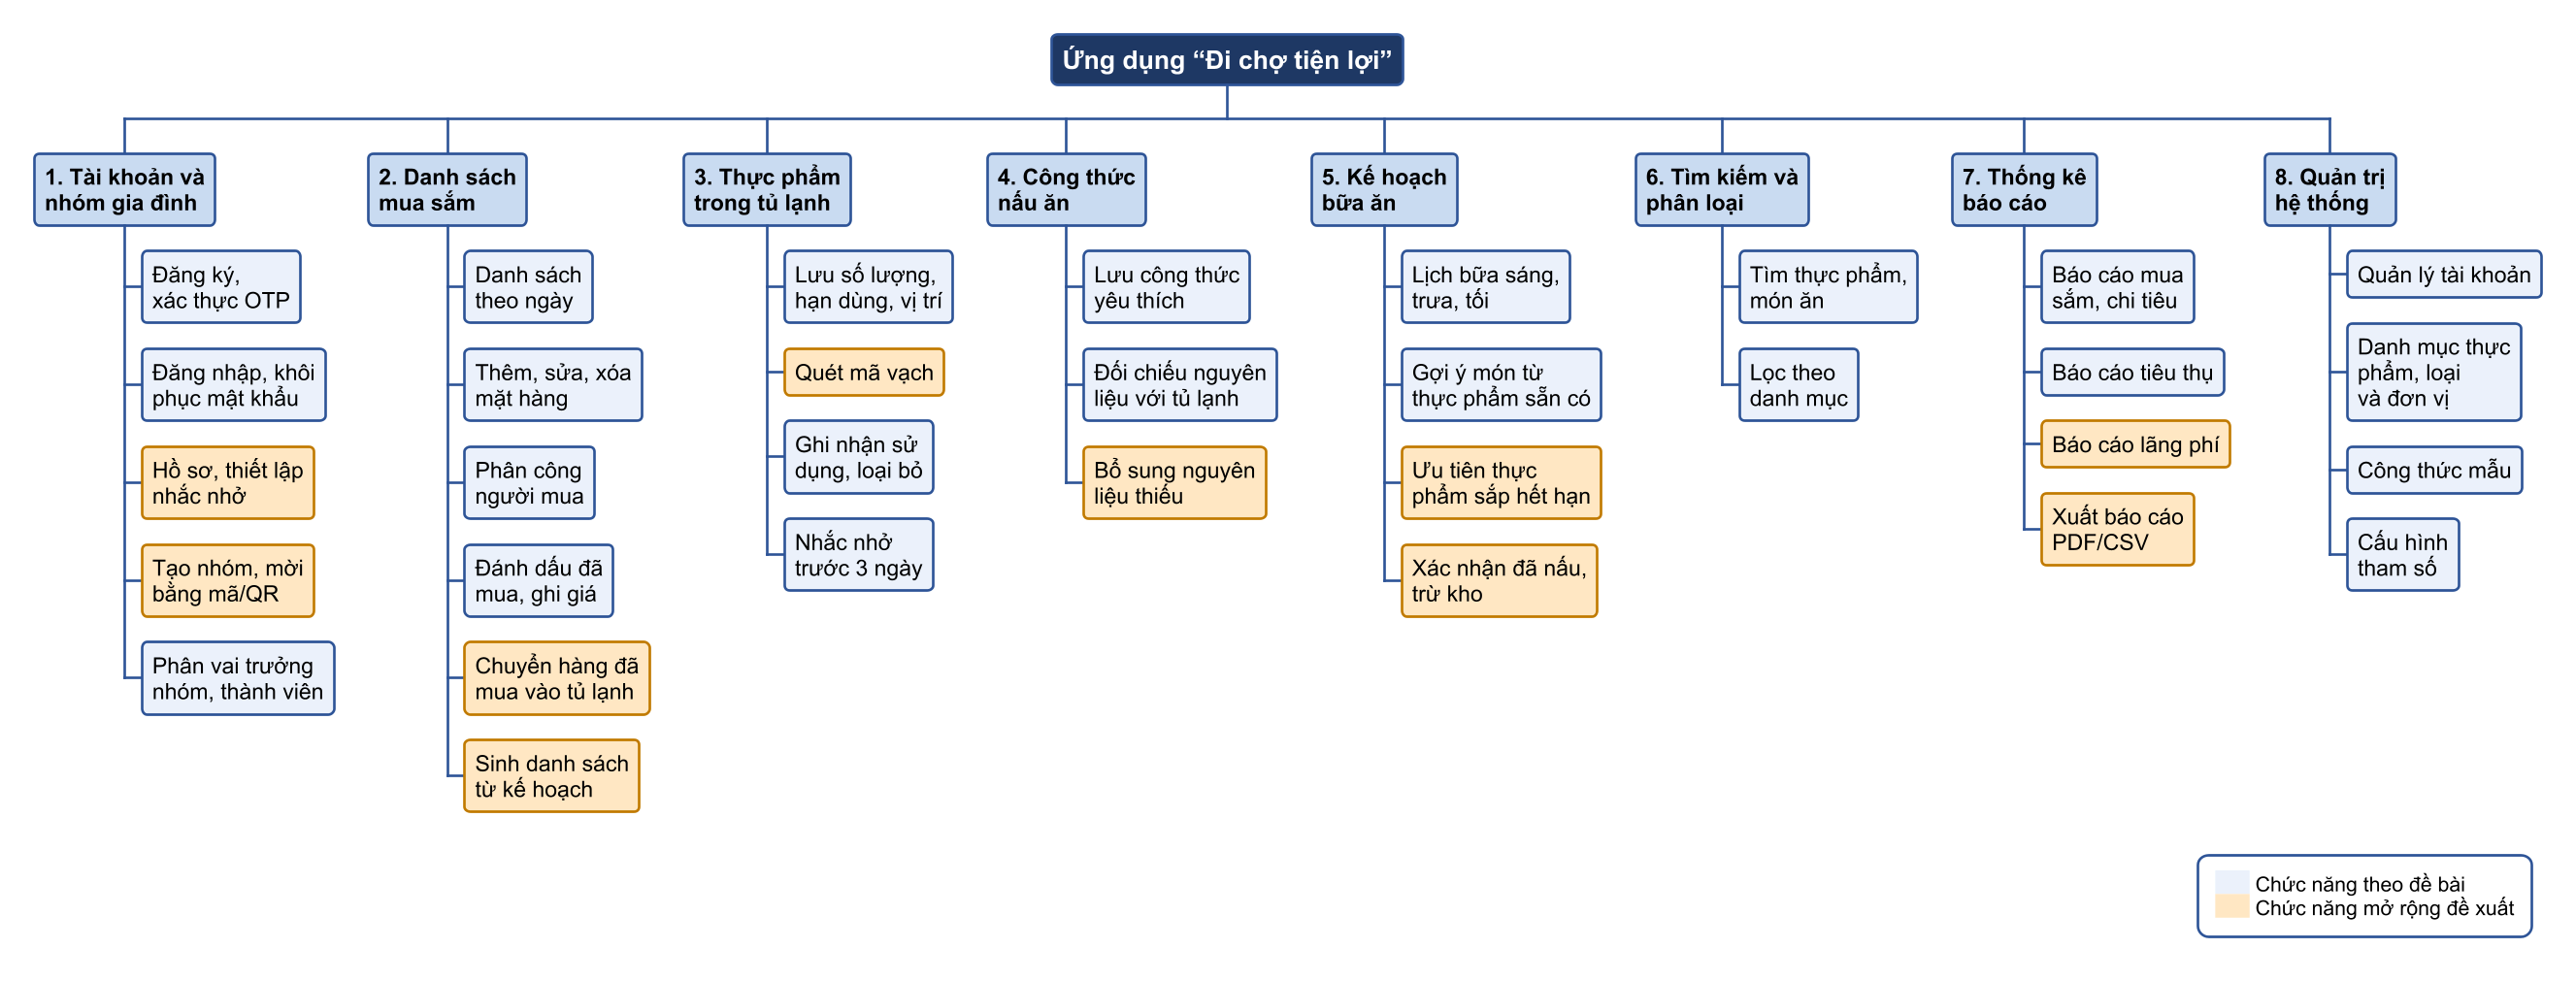
\includegraphics[width=\linewidth,height=0.85\textheight,keepaspectratio]{c1-03-phan-ra-chuc-nang}
  \caption{Sơ đồ phân rã chức năng của ứng dụng}\label{fig:phan-ra-chuc-nang}
\end{figure}

Ngoài các chức năng trong đề bài, nhóm đề xuất một số chức năng mở rộng, được đánh dấu màu cam trong Hình~\ref{fig:phan-ra-chuc-nang} và liệt kê tại Bảng~\ref{tab:chuc-nang-mo-rong}. Các chức năng này liên kết các khâu trong quy trình: mặt hàng đã mua có thể được chuyển vào tủ lạnh cùng hạn dùng đề xuất; nguyên liệu được trừ khỏi tồn kho khi người dùng xác nhận đã nấu; phần nguyên liệu còn thiếu được đưa vào danh sách mua sắm khi lập kế hoạch bữa ăn. Nhờ đó, dữ liệu được tái sử dụng giữa các khâu thay vì phải nhập lại.

{\small
\begin{longtable}{|C{1.1cm}|L{3.7cm}|L{\dimexpr\textwidth-8\tabcolsep-5\arrayrulewidth-1.1cm-3.7cm-2.1cm\relax}|C{2.1cm}|}
\caption{Các chức năng mở rộng đề xuất}\label{tab:chuc-nang-mo-rong}\\
\hline
\hd{Mã} & \hd{Chức năng mở rộng} & \hd{Vấn đề được giải quyết} & \hd{Use case}\\ \hline
\endfirsthead
\multicolumn{4}{l}{\footnotesize\itshape Bảng \thetable\ (tiếp theo)}\\ \hline
\hd{Mã} & \hd{Chức năng mở rộng} & \hd{Vấn đề được giải quyết} & \hd{Use case}\\ \hline
\endhead
MR01 & Mời thành viên bằng mã mời hoặc mã QR & Thành viên gia nhập nhóm nhanh, không cần trưởng nhóm biết trước email; mã có thời hạn và có thể thu hồi để bảo đảm an toàn & \uc{UC10}, \uc{UC11}\\ \hline
MR02 & Chuyển mặt hàng đã mua vào tủ lạnh & Loại bỏ việc nhập lại thông tin thực phẩm sau khi đi chợ; hạn dùng được đề xuất theo loại thực phẩm và vị trí bảo quản & \uc{UC21}\\ \hline
MR03 & Sinh danh sách mua sắm từ kế hoạch bữa ăn & Chỉ mua phần nguyên liệu thực sự còn thiếu sau khi đã trừ tồn kho và các danh sách đang chờ mua & \uc{UC22}\\ \hline
MR04 & Quét mã vạch sản phẩm & Nhập nhanh thực phẩm đóng gói, giảm sai sót chính tả; tra cứu danh mục nội bộ trước, sau đó đến cơ sở dữ liệu sản phẩm mở & \uc{UC26}\\ \hline
MR05 & Gợi ý món có chấm điểm, ưu tiên thực phẩm sắp hết hạn & Biến cảnh báo hạn dùng thành hành động cụ thể: món nào nên nấu ngay để không lãng phí & \uc{UC40}\\ \hline
MR06 & Xác nhận đã nấu và trừ kho theo nguyên tắc FEFO & Tồn kho luôn phản ánh đúng thực tế mà không cần người dùng tự cập nhật từng thực phẩm & \uc{UC41}\\ \hline
MR07 & Bổ sung nguyên liệu còn thiếu từ công thức & Từ màn hình công thức, một thao tác là đưa phần còn thiếu vào danh sách mua sắm & \uc{UC36}\\ \hline
MR08 & Báo cáo chi tiêu, báo cáo lãng phí và xuất báo cáo & Lượng hóa giá trị thực phẩm bị bỏ đi, giúp gia đình điều chỉnh thói quen và ngân sách & \uc{UC44}, \uc{UC46}, \uc{UC47}\\ \hline
MR09 & Thiết lập nhắc nhở cá nhân hóa & Mỗi thành viên tự chọn ngưỡng nhắc từ 1 đến 7 ngày và bật, tắt từng loại thông báo; mặc định vẫn là 3 ngày theo đề bài & \uc{UC08}\\ \hline
MR10 & Đồng bộ thời gian thực và hoạt động ngoại tuyến & Danh sách vẫn dùng được tại chợ hoặc siêu thị khi sóng yếu; thay đổi được đồng bộ khi có mạng trở lại & \nfr{NFR10}, \nfr{NFR11}\\ \hline
\end{longtable}
}

Hình~\ref{fig:chu-trinh} minh họa chu trình nghiệp vụ đề xuất. Chu trình bắt đầu từ lập kế hoạch bữa ăn, tiếp tục qua các khâu tạo danh sách, phân công mua sắm, nhập thực phẩm vào tủ lạnh, theo dõi hạn dùng và nấu ăn, rồi kết thúc bằng thống kê. Kết quả thống kê được dùng để điều chỉnh kế hoạch tiếp theo. Mũi tên nét đứt biểu thị việc thông tin về thực phẩm sắp hết hạn được sử dụng để ưu tiên gợi ý món trong bước lập kế hoạch.

\diagram[\textwidth]{c1-02-chu-trinh-nghiep-vu}{Chu trình nghiệp vụ khép kín đề xuất cho ứng dụng}{fig:chu-trinh}

% ---------------------------------------------------------------------
\section{Xác định thông tin cơ bản cho nghiệp vụ của bài toán}\label{sec:thong-tin-nghiep-vu}

Phần này phân tích bài toán ở mức nghiệp vụ, độc lập với giải pháp công nghệ. Sơ đồ ngữ cảnh được dùng để xác định ranh giới hệ thống và các bên tương tác. Tiếp đó, bài toán được chia thành tám nhóm nghiệp vụ; các nghiệp vụ con trong từng nhóm được phân tích theo mô hình Đầu vào – Xử lý – Đầu ra (Input – Process – Output, IPO). Cuối cùng, các khái niệm và ràng buộc nghiệp vụ được tổng hợp thành mô hình khái niệm và bảng quy tắc nghiệp vụ.

\subsection{Ngữ cảnh hệ thống và các nhóm nghiệp vụ}\label{ssec:ngu-canh}

Hình~\ref{fig:ngu-canh} xác định ranh giới hệ thống “Đi chợ tiện lợi”, gồm ứng dụng di động trên thiết bị người dùng và máy chủ lưu trữ dữ liệu tập trung. Các bên tương tác trực tiếp gồm khách chưa có tài khoản, người dùng, thành viên gia đình, trưởng nhóm và quản trị viên. Hệ thống phụ thuộc vào ba dịch vụ bên ngoài: dịch vụ thông báo đẩy, dịch vụ thư điện tử để gửi mã xác thực và thư khôi phục mật khẩu, và cơ sở dữ liệu sản phẩm mở để tra cứu mã vạch~\cite{openfoodfacts}. Ngoài ra, bộ lập lịch kích hoạt tác vụ kiểm tra hạn sử dụng hằng ngày.

\diagram[0.95\textwidth]{c1-04-ngu-canh}{Sơ đồ ngữ cảnh của hệ thống}{fig:ngu-canh}

Ở mức tổng quát, hệ thống tiếp nhận thông tin về người dùng, mặt hàng, thực phẩm, công thức và kế hoạch bữa ăn. Hệ thống xử lý dữ liệu bằng các cơ chế hợp nhất, phân công, theo dõi hạn dùng, chấm điểm gợi ý và tổng hợp số liệu; đầu ra gồm danh sách mua sắm có phân công, tồn kho kèm trạng thái hạn dùng, thông báo, lịch bữa ăn và báo cáo. Mô hình IPO được trình bày ở Hình~\ref{fig:ipo-tong-quat}.

\diagram[\textwidth]{c1-05-ipo-tong-quat}{Mô hình Đầu vào – Xử lý – Đầu ra tổng quát của hệ thống}{fig:ipo-tong-quat}

Từ đề bài và chu trình nghiệp vụ ở Hình~\ref{fig:chu-trinh}, bài toán được chia thành tám nhóm nghiệp vụ như trình bày tại Bảng~\ref{tab:nhom-nghiep-vu}. Mã nhóm được sử dụng xuyên suốt báo cáo để truy vết tới các use case ở Chương~\ref{chap:dac-ta} và ma trận truy vết ở Phụ lục~\ref{pl:truy-vet}.

{\small
\begin{longtable}{|C{1.3cm}|L{4.2cm}|L{\dimexpr\textwidth-6\tabcolsep-4\arrayrulewidth-1.3cm-4.2cm\relax}|}
\caption{Các nhóm nghiệp vụ của bài toán}\label{tab:nhom-nghiep-vu}\\
\hline
\hd{Mã} & \hd{Nhóm nghiệp vụ} & \hd{Mục đích}\\ \hline
\endfirsthead
\multicolumn{3}{l}{\footnotesize\itshape Bảng \thetable\ (tiếp theo)}\\ \hline
\hd{Mã} & \hd{Nhóm nghiệp vụ} & \hd{Mục đích}\\ \hline
\endhead
NV01 & Quản lý tài khoản và nhóm gia đình & Định danh người dùng, tổ chức người dùng thành nhóm gia đình với vai trò rõ ràng làm cơ sở chia sẻ dữ liệu và phân quyền\\ \hline
NV02 & Quản lý danh sách mua sắm & Tổng hợp nhu cầu mua sắm theo ngày, phân công và theo dõi tiến độ mua của cả gia đình\\ \hline
NV03 & Quản lý thực phẩm trong tủ lạnh & Duy trì tồn kho thực phẩm chính xác theo số lượng, vị trí, hạn dùng và cảnh báo trước khi hết hạn\\ \hline
NV04 & Quản lý công thức nấu ăn & Lưu trữ công thức yêu thích và liên kết nguyên liệu của công thức với tồn kho\\ \hline
NV05 & Lập kế hoạch bữa ăn và gợi ý món & Lên lịch bữa sáng, trưa, tối theo ngày hoặc tuần, gợi ý món từ thực phẩm sẵn có\\ \hline
NV06 & Tìm kiếm và phân loại thực phẩm & Tra cứu nhanh thực phẩm, món ăn trong danh mục hệ thống hoặc trong tủ lạnh theo danh mục\\ \hline
NV07 & Thống kê báo cáo & Tổng hợp số liệu mua sắm, chi tiêu, tiêu thụ và lãng phí theo khoảng thời gian\\ \hline
NV08 & Quản trị hệ thống & Quản lý tài khoản, dữ liệu danh mục dùng chung và tham số vận hành của hệ thống\\ \hline
\end{longtable}
}

\subsection{Nghiệp vụ quản lý tài khoản và nhóm gia đình}\label{ssec:nv01}

NV01 quản lý tài khoản và quyền truy cập của người dùng. Người dùng đăng ký bằng email và xác thực địa chỉ này qua mã OTP. Sau khi tài khoản được kích hoạt, hệ thống tạo một \emph{không gian cá nhân} — một nhóm chỉ có một thành viên — để người dùng có thể sử dụng ứng dụng mà không cần tham gia nhóm gia đình. Khi muốn chia sẻ dữ liệu, người dùng có thể tạo nhóm gia đình, trở thành trưởng nhóm và mời thành viên khác bằng mã mời hoặc mã QR. Mọi danh sách mua sắm, tồn kho và kế hoạch bữa ăn đều gắn với một nhóm, dù là không gian cá nhân hay nhóm gia đình. Các nghiệp vụ con được trình bày trong Bảng~\ref{tab:nv01}.

\begin{nvtable}{Phân rã nghiệp vụ NV01 – Quản lý tài khoản và nhóm gia đình}{tab:nv01}
\nvrow{NV01.1}{Đăng ký tài khoản}{Họ tên, email, mật khẩu, xác nhận mật khẩu}{Kiểm tra định dạng, kiểm tra email chưa tồn tại, tạo tài khoản chờ xác thực, gửi OTP (\br{BR01}, \br{BR02})}{Tài khoản chờ xác thực, thư chứa mã OTP}
\nvrow{NV01.2}{Xác thực tài khoản}{Email, mã OTP}{So khớp mã, kiểm tra thời hạn và số lần nhập sai; kích hoạt tài khoản, tạo không gian cá nhân (\br{BR02}, \br{BR04})}{Tài khoản hoạt động, không gian cá nhân}
\nvrow{NV01.3}{Đăng nhập, khôi phục mật khẩu}{Email, mật khẩu hoặc mã OTP khôi phục, mật khẩu mới}{Đối chiếu thông tin, đếm số lần sai và khóa tạm, cấp phiên làm việc (\br{BR03})}{Phiên đăng nhập hợp lệ hoặc thông báo lỗi}
\nvrow{NV01.4}{Quản lý hồ sơ và thiết lập nhắc nhở}{Họ tên, ảnh đại diện, ngưỡng nhắc N, các loại thông báo}{Kiểm tra miền giá trị, lưu thiết lập cá nhân (\br{BR12}, \br{BR13})}{Hồ sơ và thiết lập đã cập nhật}
\nvrow{NV01.5}{Tạo nhóm gia đình}{Tên nhóm, ảnh nhóm (tùy chọn)}{Kiểm tra người dùng chưa thuộc nhóm gia đình nào, tạo nhóm, gán vai trò trưởng nhóm (\br{BR04}, \br{BR05})}{Nhóm gia đình mới, người tạo là trưởng nhóm}
\nvrow{NV01.6}{Mời và tiếp nhận thành viên}{Mã mời hoặc mã QR}{Sinh mã có thời hạn; khi người dùng nhập mã, kiểm tra hiệu lực, số thành viên tối đa và tư cách thành viên hiện tại (\br{BR05}, \br{BR06})}{Thành viên mới trong nhóm, thông báo tới trưởng nhóm}
\nvrow{NV01.7}{Điều phối thành viên}{Thành viên được chọn, thao tác xóa hoặc chuyển quyền}{Kiểm tra quyền trưởng nhóm; khi xóa hoặc rời nhóm, trả các mặt hàng đang giao về trạng thái Cần mua (\br{BR07})}{Danh sách thành viên và vai trò mới}
\end{nvtable}

\subsection{Nghiệp vụ quản lý danh sách mua sắm}\label{ssec:nv02}

NV02 quản lý danh sách mua sắm theo ngày dự kiến và không gian hiện hành của người dùng. Mỗi mặt hàng tham chiếu đến một thực phẩm trong danh mục, kèm số lượng, đơn vị và ghi chú. Nếu mặt hàng trùng thực phẩm và có cùng đơn vị hoặc đơn vị thuộc cùng nhóm đại lượng, hệ thống cộng dồn số lượng thay vì tạo dòng mới. Trưởng nhóm có thể giao mặt hàng cho một thành viên; người được giao nhận thông báo trên thiết bị. Quy trình này được mô tả ở Hình~\ref{fig:quy-trinh-mua-sam}.

\diagram[0.72\textwidth]{c1-06-quy-trinh-mua-sam-nhom}{Quy trình mua sắm có phân công trong nhóm gia đình}{fig:quy-trinh-mua-sam}

Vòng đời của mặt hàng được biểu diễn ở Hình~\ref{fig:trang-thai-mat-hang}. Mặt hàng bắt đầu ở trạng thái \emph{Cần mua}, chuyển sang \emph{Đã phân công} khi được giao cho thành viên và sang \emph{Đã mua} khi có người đánh dấu. Sau đó, mặt hàng chuyển sang \emph{Đã nhập tủ lạnh} nếu được đưa vào tủ, hoặc \emph{Đã bỏ qua} nếu gia đình quyết định không mua. Trước khi nhập tủ, người dùng có thể hoàn tác trạng thái \emph{Đã mua} về \emph{Cần mua} để sửa thao tác nhầm. Trạng thái danh sách được suy ra từ trạng thái các mặt hàng: \emph{Đang lập} nếu chưa có mặt hàng nào được mua, \emph{Đang mua} nếu có ít nhất một mặt hàng đã mua và \emph{Hoàn tất} khi mọi mặt hàng đã được xử lý.

\diagram[0.58\textwidth]{c1-07-trang-thai-mat-hang}{Vòng đời của một mặt hàng trong danh sách mua sắm}{fig:trang-thai-mat-hang}

Các nghiệp vụ con của NV02 được phân tích trong Bảng~\ref{tab:nv02}.

\begin{nvtable}{Phân rã nghiệp vụ NV02 – Quản lý danh sách mua sắm}{tab:nv02}
\nvrow{NV02.1}{Tạo danh sách mua sắm}{Tên danh sách, ngày dự kiến mua, ghi chú}{Kiểm tra ngày không ở quá khứ, gắn danh sách vào không gian hiện hành (\br{BR08})}{Danh sách ở trạng thái Đang lập}
\nvrow{NV02.2}{Cập nhật mặt hàng}{Thực phẩm, số lượng, đơn vị, ghi chú}{Gợi ý tên từ danh mục; phát hiện trùng và gộp số lượng sau khi quy đổi đơn vị (\br{BR09}, \br{BR16})}{Mặt hàng mới hoặc mặt hàng đã gộp, danh sách được đồng bộ}
\nvrow{NV02.3}{Tái sử dụng danh sách}{Danh sách nguồn, ngày mua mới}{Sao chép các mặt hàng, đặt lại trạng thái Cần mua và bỏ phân công cũ}{Danh sách mới dựa trên danh sách cũ}
\nvrow{NV02.4}{Phân công người mua}{Mặt hàng, thành viên được giao}{Kiểm tra vai trò trưởng nhóm, mỗi mặt hàng giao tối đa một người, gửi thông báo đẩy (\br{BR10})}{Mặt hàng Đã phân công, thông báo tới người được giao}
\nvrow{NV02.5}{Ghi nhận đã mua}{Mặt hàng, số lượng thực tế, đơn giá}{Xác nhận khi mua thay người được giao; ghi người mua, thời điểm; cập nhật trạng thái danh sách (\br{BR08}, \br{BR10})}{Mặt hàng Đã mua, dữ liệu chi tiêu}
\nvrow{NV02.6}{Chuyển vào tủ lạnh}{Mặt hàng đã mua, vị trí lưu trữ, ngày hết hạn}{Đề xuất hạn dùng theo thực phẩm và vị trí, tạo lô thực phẩm trong tủ (\br{BR11})}{Lô thực phẩm mới, mặt hàng Đã nhập tủ lạnh}
\nvrow{NV02.7}{Sinh danh sách từ kế hoạch}{Khoảng ngày trong lịch bữa ăn}{Tổng hợp nhu cầu nguyên liệu, trừ tồn kho và lượng đang chờ mua (\br{BR20})}{Danh sách mua sắm cho phần còn thiếu}
\end{nvtable}

\subsection{Nghiệp vụ quản lý thực phẩm trong tủ lạnh}\label{ssec:nv03}

NV03 theo dõi tồn kho thực phẩm trong tủ lạnh. Đơn vị quản lý là \emph{lô thực phẩm}: mỗi lần nhập thực phẩm — bằng cách nhập tay, quét mã vạch hoặc chuyển từ danh sách mua sắm — hệ thống tạo một lô riêng với số lượng, đơn vị, ngày mua, ngày hết hạn và vị trí lưu trữ. Quản lý theo lô giúp phân biệt các thực phẩm cùng loại nhưng có ngày hết hạn khác nhau, chẳng hạn hai hộp sữa mua vào những thời điểm khác nhau. Vị trí lưu trữ gồm năm giá trị chuẩn; mỗi vị trí ảnh hưởng đến hạn dùng gợi ý như trình bày tại Bảng~\ref{tab:vi-tri-luu-tru}.

{\small
\begin{longtable}{|L{2.6cm}|L{3.2cm}|L{\dimexpr\textwidth-8\tabcolsep-5\arrayrulewidth-2.6cm-3.2cm-4.8cm\relax}|L{4.8cm}|}
\caption{Vị trí lưu trữ và hạn dùng gợi ý mặc định}\label{tab:vi-tri-luu-tru}\\
\hline
\hd{Vị trí} & \hd{Điều kiện bảo quản} & \hd{Nhóm thực phẩm điển hình} & \hd{Ví dụ hạn dùng gợi ý mặc định}\\ \hline
\endfirsthead
\multicolumn{4}{l}{\footnotesize\itshape Bảng \thetable\ (tiếp theo)}\\ \hline
\hd{Vị trí} & \hd{Điều kiện bảo quản} & \hd{Nhóm thực phẩm điển hình} & \hd{Ví dụ hạn dùng gợi ý mặc định}\\ \hline
\endhead
Ngăn mát & Khoảng 0–4~°C & Thịt, cá tươi, đồ ăn đã nấu, sữa đã mở nắp & Thịt gia cầm, cá tươi: 2 ngày; thịt bò, lợn miếng: 3 ngày; đồ ăn đã nấu: 3 ngày\\ \hline
Ngăn đông & Từ −18~°C trở xuống & Thịt, cá cấp đông, đồ đông lạnh & Thịt xay, cá: 90 ngày; thịt miếng: 120 ngày\\ \hline
Ngăn rau củ & Ngăn mát, độ ẩm cao & Rau lá, củ, quả & Rau lá xanh: 4 ngày; cà rốt, củ cải: 14 ngày\\ \hline
Cánh tủ & Nhiệt độ dao động nhiều hơn & Trứng, đồ uống, gia vị dạng lỏng & Trứng gà: 21 ngày; nước sốt đã mở: 30 ngày\\ \hline
Kệ bếp, tủ khô & Nhiệt độ phòng, khô ráo & Gạo, mì khô, đồ hộp, gia vị khô & Theo hạn in trên bao bì\\ \hline
\end{longtable}
}

Các giá trị trong Bảng~\ref{tab:vi-tri-luu-tru} là giá trị mặc định nhằm giảm thao tác nhập liệu, được xây dựng dựa trên khuyến nghị bảo quản thực phẩm của cơ quan an toàn thực phẩm Hoa Kỳ~\cite{usdafoodkeeper}. Quản trị viên có thể điều chỉnh các giá trị này trong danh mục thực phẩm; người dùng cũng có thể sửa theo hạn sử dụng ghi trên bao bì.

Trạng thái hạn dùng được xác định theo số ngày còn lại $d$ và ngưỡng nhắc $N$ của người dùng (mặc định $N = 3$). Lô ở trạng thái \emph{Còn hạn} khi $d > N$, \emph{Sắp hết hạn} khi $0 \le d \le N$ và \emph{Đã hết hạn} khi $d < 0$. Ví dụ, thực phẩm hết hạn ngày 10 sẽ bắt đầu được nhắc từ ngày 7. Vòng đời của lô được thể hiện ở Hình~\ref{fig:trang-thai-thuc-pham}. Trạng thái có thể chuyển từ \emph{Sắp hết hạn} về \emph{Còn hạn} nếu người dùng cập nhật hạn dùng, chẳng hạn khi chuyển thịt từ ngăn mát sang ngăn đông.

\diagram[0.56\textwidth]{c1-08-trang-thai-thuc-pham}{Vòng đời của một lô thực phẩm trong tủ lạnh}{fig:trang-thai-thuc-pham}

Mọi thay đổi về số lượng của lô được ghi vào \emph{nhật ký sử dụng}, gồm hai loại: \emph{tiêu thụ} khi thực phẩm được dùng để nấu ăn và \emph{loại bỏ} khi thực phẩm bị hỏng hoặc hết hạn. Nhật ký này cung cấp dữ liệu cho các báo cáo tiêu thụ và lãng phí trong NV07. Các nghiệp vụ con của NV03 được trình bày tại Bảng~\ref{tab:nv03}.

\begin{nvtable}{Phân rã nghiệp vụ NV03 – Quản lý thực phẩm trong tủ lạnh}{tab:nv03}
\nvrow{NV03.1}{Nhập thực phẩm vào tủ}{Thực phẩm hoặc mã vạch, số lượng, đơn vị, ngày mua, ngày hết hạn, vị trí}{Tra cứu danh mục theo tên hoặc mã vạch; đề xuất hạn dùng nếu bỏ trống; kiểm tra ngày hết hạn không trước ngày mua (\br{BR11}, \br{BR14})}{Lô thực phẩm mới ở trạng thái tương ứng}
\nvrow{NV03.2}{Cập nhật lô thực phẩm}{Lô thực phẩm, thông tin thay đổi}{Kiểm tra hợp lệ, tính lại trạng thái hạn dùng (\br{BR12})}{Lô thực phẩm đã cập nhật}
\nvrow{NV03.3}{Ghi nhận sử dụng}{Thực phẩm, lượng sử dụng}{Trừ theo nguyên tắc hết hạn trước dùng trước, không cho lượng âm; ghi nhật ký tiêu thụ (\br{BR14}, \br{BR15})}{Tồn kho mới, bản ghi tiêu thụ}
\nvrow{NV03.4}{Loại bỏ thực phẩm}{Lô thực phẩm, lượng loại bỏ, lý do}{Trừ tồn kho, ghi nhật ký loại bỏ kèm giá trị ước tính (\br{BR21})}{Lô Đã loại bỏ hoặc giảm số lượng, bản ghi lãng phí}
\nvrow{NV03.5}{Theo dõi và nhắc hạn dùng}{Thời gian hệ thống, tồn kho, thiết lập nhắc nhở của từng thành viên}{Chạy định kỳ mỗi ngày, cập nhật trạng thái, lọc theo ngưỡng N, chống nhắc trùng trong ngày (\br{BR12}, \br{BR13})}{Thông báo tổng hợp gửi tới từng thành viên}
\end{nvtable}

\subsection{Nghiệp vụ quản lý công thức nấu ăn}\label{ssec:nv04}

NV04 cho phép người dùng lưu trữ công thức nấu ăn. Mỗi công thức gồm tên món, ảnh minh họa, số khẩu phần chuẩn, thời gian chuẩn bị và nấu, các bước thực hiện và danh sách nguyên liệu. Mỗi nguyên liệu được liên kết với một thực phẩm trong danh mục, kèm số lượng và đơn vị, thay vì chỉ được ghi dưới dạng văn bản tự do. Nhờ đó, hệ thống có thể đối chiếu công thức với tồn kho, xác định nguyên liệu còn thiếu và điều chỉnh lượng nguyên liệu theo số khẩu phần. Nguyên liệu được phân thành loại bắt buộc và tùy chọn để việc đánh giá khả năng chế biến linh hoạt hơn. Ngoài công thức do người dùng tạo, hệ thống cung cấp bộ công thức mẫu do quản trị viên biên soạn. Các nghiệp vụ con của NV04 được trình bày tại Bảng~\ref{tab:nv04}.

\begin{nvtable}{Phân rã nghiệp vụ NV04 – Quản lý công thức nấu ăn}{tab:nv04}
\nvrow{NV04.1}{Tạo và cập nhật công thức}{Tên món, ảnh, khẩu phần, thời gian, các bước, nguyên liệu kèm định lượng}{Kiểm tra trường bắt buộc, ít nhất một nguyên liệu, liên kết nguyên liệu với danh mục (\br{BR16}, \br{BR17})}{Công thức trong bộ sưu tập của người dùng}
\nvrow{NV04.2}{Đối chiếu nguyên liệu với tủ lạnh}{Công thức, số khẩu phần mong muốn, tồn kho}{Nhân tỷ lệ định lượng, quy đổi đơn vị, so sánh với lượng còn hạn trong tủ (\br{BR15}, \br{BR16})}{Nhãn Đủ hoặc Thiếu cho từng nguyên liệu}
\nvrow{NV04.3}{Bổ sung nguyên liệu thiếu}{Kết quả đối chiếu, danh sách mua sắm đích}{Đưa phần thiếu vào danh sách, gộp nếu trùng (\br{BR09})}{Mặt hàng mới trong danh sách mua sắm}
\nvrow{NV04.4}{Đánh dấu yêu thích, sao chép công thức mẫu}{Công thức}{Ghi nhận yêu thích; sao chép công thức mẫu thành bản riêng có thể chỉnh sửa (\br{BR17})}{Bộ sưu tập công thức cá nhân hóa}
\end{nvtable}

\subsection{Nghiệp vụ lập kế hoạch bữa ăn và gợi ý món}\label{ssec:nv05}

NV05 hỗ trợ lập kế hoạch bữa ăn theo lịch. Mỗi ngày gồm ba bữa sáng, trưa và tối; mỗi bữa có thể có nhiều món, trong đó mỗi món liên kết với một công thức và số khẩu phần. Người dùng có thể xem kế hoạch theo ngày hoặc tuần để dự trù nguyên liệu. Quy trình lập kế hoạch gắn với tồn kho được trình bày ở Hình~\ref{fig:quy-trinh-ke-hoach}.

\diagram[0.6\textwidth]{c1-09-quy-trinh-ke-hoach-bua-an}{Quy trình lập kế hoạch bữa ăn gắn với tồn kho}{fig:quy-trinh-ke-hoach}

Gợi ý món là nghiệp vụ có nhiều bước xử lý nhất trong nhóm này. Với mỗi công thức ứng viên $c$, hệ thống tính ba đại lượng. Tỷ lệ đáp ứng $R(c)$ bằng tỷ số giữa số nguyên liệu bắt buộc hiện có đủ trong tủ và tổng số nguyên liệu bắt buộc của công thức. Điểm ưu tiên hạn dùng $E(c)$ phản ánh khả năng sử dụng thực phẩm sắp hết hạn và được tính như sau:
\begin{equation}\label{eq:diem-han-dung}
E(c) = \min\Bigl(1,\ \sum_{i \in I_c} w_i\Bigr), \qquad
w_i =
\begin{cases}
\dfrac{N + 1 - d_i}{N + 1} & \text{nếu } 0 \le d_i \le N,\\[6pt]
0 & \text{trong các trường hợp còn lại,}
\end{cases}
\end{equation}
trong đó $I_c$ là tập nguyên liệu của công thức có trong tủ và $d_i$ là số ngày còn lại của lô gần hết hạn nhất ứng với nguyên liệu $i$. Trọng số $w_i$ càng lớn khi thực phẩm càng gần ngày hết hạn. Đại lượng thứ ba $F(c)$ nhận giá trị 1 nếu công thức được người dùng đánh dấu yêu thích và 0 nếu ngược lại. Điểm gợi ý tổng hợp được xác định theo công thức
\begin{equation}\label{eq:diem-goi-y}
S(c) = 0{,}6\,R(c) + 0{,}3\,E(c) + 0{,}1\,F(c).
\end{equation}
Hệ thống chỉ đưa vào kết quả các công thức có $R(c) \ge \theta$ (mặc định $\theta = 0{,}6$), sau đó sắp xếp theo $S(c)$ giảm dần. Quản trị viên có thể điều chỉnh các trọng số và ngưỡng. Do $R$ có trọng số lớn nhất, công thức đáp ứng nhiều nguyên liệu được ưu tiên; khi mức đáp ứng tương đương, công thức giúp sử dụng thực phẩm sắp hết hạn được xếp cao hơn.

Khi người dùng xác nhận đã nấu, hệ thống trừ nguyên liệu khỏi tồn kho theo nguyên tắc \emph{hết hạn trước, dùng trước} (First Expired, First Out – FEFO): với mỗi nguyên liệu, lô có ngày hết hạn sớm nhất được trừ trước. Cách xử lý này ưu tiên sử dụng thực phẩm gần hết hạn và hạn chế bỏ quên các lô cũ. Các nghiệp vụ con của NV05 được tổng hợp tại Bảng~\ref{tab:nv05}.

\begin{nvtable}{Phân rã nghiệp vụ NV05 – Lập kế hoạch bữa ăn và gợi ý món}{tab:nv05}
\nvrow{NV05.1}{Lên lịch bữa ăn}{Ngày, bữa, công thức, số khẩu phần}{Kiểm tra ngày trong khoảng cho phép, thêm món vào bữa (\br{BR18})}{Bữa ăn dự kiến trong lịch}
\nvrow{NV05.2}{Xem và điều chỉnh lịch}{Ngày hoặc tuần cần xem, thao tác sửa, xóa}{Tổng hợp theo ngày, đánh dấu món đã đủ hoặc thiếu nguyên liệu (\br{BR18})}{Lịch bữa ăn theo ngày hoặc tuần}
\nvrow{NV05.3}{Gợi ý món ăn}{Tồn kho khả dụng, tập công thức, bữa và khẩu phần mong muốn}{Tính $R$, $E$, $F$, lọc theo ngưỡng $\theta$, xếp hạng theo $S$ (\br{BR19})}{Tối đa 10 món gợi ý kèm nguyên liệu thiếu}
\nvrow{NV05.4}{Xác nhận đã nấu}{Bữa ăn, khẩu phần thực tế, điều chỉnh lượng dùng}{Tính lượng nguyên liệu, trừ kho theo FEFO, ghi nhật ký tiêu thụ (\br{BR14}, \br{BR15})}{Bữa ăn Đã nấu, tồn kho mới}
\end{nvtable}

\subsection{Nghiệp vụ tìm kiếm và phân loại thực phẩm}\label{ssec:nv06}

NV06 hỗ trợ tra cứu trong danh mục thực phẩm, tủ lạnh và bộ sưu tập công thức. Tìm kiếm không phân biệt dấu (ví dụ, “ca rot” khớp với “cà rốt”); kết quả có thể lọc theo loại thực phẩm, vị trí lưu trữ và trạng thái hạn dùng. Danh mục thực phẩm gồm hai cấp: loại thực phẩm (thịt, hải sản, rau củ, trái cây, trứng và sữa, đồ khô, đồ hộp, gia vị, đồ uống) và thực phẩm cụ thể. Bảng~\ref{tab:nv06} tóm tắt các nghiệp vụ con.

\begin{nvtable}{Phân rã nghiệp vụ NV06 – Tìm kiếm và phân loại thực phẩm}{tab:nv06}
\nvrow{NV06.1}{Tìm kiếm thực phẩm, món ăn}{Từ khóa, phạm vi tìm (danh mục, tủ lạnh, công thức)}{Chuẩn hóa bỏ dấu, so khớp theo tiền tố và từ khóa, xếp hạng theo độ liên quan}{Danh sách kết quả có phân trang}
\nvrow{NV06.2}{Lọc theo danh mục}{Loại thực phẩm, vị trí, trạng thái hạn dùng}{Kết hợp điều kiện lọc với kết quả tìm kiếm}{Danh sách đã lọc, số lượng theo từng nhóm}
\nvrow{NV06.3}{Gợi ý từ thực phẩm sẵn có}{Tồn kho hiện tại}{Dùng chung cơ chế chấm điểm của NV05.3 (\br{BR19})}{Danh sách món phù hợp}
\end{nvtable}

\subsection{Nghiệp vụ thống kê báo cáo}\label{ssec:nv07}

NV07 tổng hợp dữ liệu từ các nghiệp vụ khác thành thông tin phục vụ việc theo dõi và ra quyết định. Báo cáo sử dụng đơn giá ghi nhận khi đánh dấu đã mua, nhật ký tiêu thụ khi nấu ăn và nhật ký loại bỏ khi thực phẩm hỏng; người dùng không cần nhập thêm dữ liệu. Các chỉ số và cách tính được trình bày tại Bảng~\ref{tab:chi-so-bao-cao}.

{\small
\begin{longtable}{|L{3.6cm}|L{\dimexpr\textwidth-6\tabcolsep-4\arrayrulewidth-3.6cm-3.4cm\relax}|L{3.4cm}|}
\caption{Các chỉ số thống kê và cách tính}\label{tab:chi-so-bao-cao}\\
\hline
\hd{Chỉ số} & \hd{Cách tính trong khoảng thời gian $[t_1, t_2]$} & \hd{Nguồn dữ liệu}\\ \hline
\endfirsthead
\multicolumn{3}{l}{\footnotesize\itshape Bảng \thetable\ (tiếp theo)}\\ \hline
\hd{Chỉ số} & \hd{Cách tính trong khoảng thời gian $[t_1, t_2]$} & \hd{Nguồn dữ liệu}\\ \hline
\endhead
Tổng chi tiêu & Tổng của số lượng nhân đơn giá trên các mặt hàng có thời điểm mua thuộc khoảng & Mặt hàng Đã mua\\ \hline
Cơ cấu chi tiêu theo loại & Tổng chi tiêu nhóm theo loại thực phẩm, biểu diễn bằng tỷ lệ phần trăm & Mặt hàng Đã mua, danh mục\\ \hline
Mặt hàng mua nhiều nhất & Mười thực phẩm có số lần mua hoặc tổng chi tiêu lớn nhất & Mặt hàng Đã mua\\ \hline
Lượng tiêu thụ & Tổng lượng tiêu thụ theo thực phẩm hoặc theo loại, quy đổi về đơn vị cơ sở & Nhật ký tiêu thụ\\ \hline
Giá trị lãng phí & Tổng của lượng loại bỏ nhân đơn giá mua của lô tương ứng, nếu lô có nguồn gốc từ mặt hàng đã ghi giá & Nhật ký loại bỏ, mặt hàng liên kết\\ \hline
Tỷ lệ lãng phí & Số lô bị loại bỏ chia cho số lô được nhập vào tủ trong khoảng, tính theo phần trăm & Nhật ký loại bỏ, lô thực phẩm\\ \hline
\end{longtable}
}

Các nghiệp vụ con của NV07 được phân tích trong Bảng~\ref{tab:nv07}.

\begin{nvtable}{Phân rã nghiệp vụ NV07 – Thống kê báo cáo}{tab:nv07}
\nvrow{NV07.1}{Báo cáo mua sắm và chi tiêu}{Khoảng thời gian, cách nhóm (ngày, tuần, tháng)}{Tổng hợp chi tiêu, cơ cấu theo loại, mặt hàng mua nhiều (\br{BR21})}{Biểu đồ cột, biểu đồ tròn, bảng chi tiết}
\nvrow{NV07.2}{Báo cáo tiêu thụ}{Khoảng thời gian, loại thực phẩm}{Tổng hợp nhật ký tiêu thụ theo thực phẩm, loại và bữa ăn}{Biểu đồ xu hướng tiêu thụ}
\nvrow{NV07.3}{Báo cáo lãng phí}{Khoảng thời gian}{Tổng hợp nhật ký loại bỏ, tính giá trị và tỷ lệ lãng phí (\br{BR21})}{Chỉ số lãng phí, danh sách thực phẩm hay bị bỏ}
\nvrow{NV07.4}{Xuất báo cáo}{Báo cáo đang xem, định dạng PDF hoặc CSV}{Kết xuất dữ liệu và biểu đồ ra tệp}{Tệp báo cáo chia sẻ được}
\end{nvtable}

\subsection{Nghiệp vụ quản trị hệ thống}\label{ssec:nv08}

NV08 dành cho quản trị viên, tập trung vào việc duy trì dữ liệu danh mục dùng chung. Chất lượng dữ liệu này ảnh hưởng đến chức năng gợi ý tên, đề xuất hạn dùng, quy đổi đơn vị và gợi ý món. Danh mục đang được dữ liệu người dùng tham chiếu không bị xóa cứng mà được chuyển sang trạng thái ngừng sử dụng để bảo toàn dữ liệu lịch sử. Quyền quản trị chỉ bao gồm thông tin tài khoản và dữ liệu danh mục; quản trị viên không được xem danh sách mua sắm, tồn kho hoặc kế hoạch bữa ăn của các gia đình. Các nghiệp vụ con được trình bày tại Bảng~\ref{tab:nv08}.

\begin{nvtable}{Phân rã nghiệp vụ NV08 – Quản trị hệ thống}{tab:nv08}
\nvrow{NV08.1}{Quản lý tài khoản người dùng}{Tiêu chí tìm kiếm, thao tác khóa, mở khóa}{Tra cứu, thay đổi trạng thái tài khoản, ghi nhật ký quản trị (\br{BR23})}{Tài khoản cập nhật trạng thái}
\nvrow{NV08.2}{Quản lý danh mục thực phẩm}{Tên, loại, đơn vị mặc định, mã vạch, hạn dùng gợi ý theo vị trí, ảnh}{Kiểm tra trùng tên trong cùng loại, kiểm tra tham chiếu trước khi ngừng sử dụng (\br{BR22})}{Danh mục thực phẩm chuẩn hóa}
\nvrow{NV08.3}{Quản lý loại mặt hàng và đơn vị đo}{Tên loại, biểu tượng; ký hiệu đơn vị, nhóm đại lượng, hệ số quy đổi}{Kiểm tra trùng, kiểm tra hệ số dương, kiểm tra tham chiếu (\br{BR16}, \br{BR22})}{Danh mục loại và đơn vị}
\nvrow{NV08.4}{Quản lý công thức mẫu}{Nội dung công thức mẫu}{Kiểm tra như NV04.1, công bố cho mọi người dùng (\br{BR17})}{Bộ công thức mẫu}
\nvrow{NV08.5}{Cấu hình tham số hệ thống}{Ngưỡng nhắc mặc định, giờ chạy nhắc nhở, số thành viên tối đa, trọng số gợi ý, thời hạn mã mời}{Kiểm tra miền giá trị, áp dụng cho các lần xử lý kế tiếp (\br{BR05}, \br{BR13}, \br{BR19})}{Bộ tham số hệ thống có hiệu lực}
\end{nvtable}

\subsection{Mô hình khái niệm và quy tắc nghiệp vụ}\label{ssec:mo-hinh-khai-niem}

Mô hình khái niệm ở Hình~\ref{fig:mo-hinh-khai-niem} tổng hợp các khái niệm nghiệp vụ cốt lõi và mối liên hệ giữa chúng. \emph{Nhóm} là khái niệm trung tâm, đại diện cho không gian cá nhân hoặc nhóm gia đình, đồng thời sở hữu danh sách mua sắm, các lô thực phẩm và bữa ăn dự kiến. Quan hệ nhiều – nhiều giữa người dùng và nhóm được thể hiện qua khái niệm \emph{Thành viên nhóm}, lưu vai trò trưởng nhóm hoặc thành viên. \emph{Thực phẩm (danh mục)} là danh mục dùng chung được tham chiếu bởi mặt hàng mua sắm, lô thực phẩm và nguyên liệu công thức, qua đó liên kết dữ liệu giữa các nghiệp vụ. Liên kết “tạo ra” giữa mặt hàng mua sắm và lô thực phẩm lưu nguồn gốc của lô để phục vụ tính toán giá trị lãng phí. Thuộc tính chi tiết của các khái niệm được mô tả trong Phụ lục~\ref{pl:tu-dien}.

\diagram[0.95\textwidth]{c1-10-mo-hinh-khai-niem}{Mô hình khái niệm nghiệp vụ}{fig:mo-hinh-khai-niem}

Các ràng buộc của hệ thống được tập hợp thành bộ quy tắc nghiệp vụ trong Bảng~\ref{tab:quy-tac-nghiep-vu}. Mỗi quy tắc có mã định danh và được tham chiếu trong đặc tả use case ở Chương~\ref{chap:dac-ta}, giúp xác định các use case liên quan khi quy tắc thay đổi.

{\small
\begin{longtable}{|C{1.25cm}|L{3.0cm}|L{\dimexpr\textwidth-6\tabcolsep-4\arrayrulewidth-1.25cm-3.0cm\relax}|}
\caption{Các quy tắc nghiệp vụ}\label{tab:quy-tac-nghiep-vu}\\
\hline
\hd{Mã} & \hd{Chủ đề} & \hd{Nội dung quy tắc}\\ \hline
\endfirsthead
\multicolumn{3}{l}{\footnotesize\itshape Bảng \thetable\ (tiếp theo)}\\ \hline
\hd{Mã} & \hd{Chủ đề} & \hd{Nội dung quy tắc}\\ \hline
\endhead
BR01 & Thông tin tài khoản & Email là duy nhất trong hệ thống và đúng định dạng; mật khẩu dài 8–32 ký tự, chứa ít nhất một chữ hoa, một chữ thường và một chữ số; họ tên dài 2–50 ký tự.\\ \hline
BR02 & Mã OTP & Mã gồm 6 chữ số, hiệu lực 5 phút, tối đa 5 lần nhập sai cho mỗi mã; chỉ được yêu cầu gửi lại sau ít nhất 60 giây và không quá 5 lần trong một giờ.\\ \hline
BR03 & Đăng nhập và phiên & Đăng nhập sai 5 lần liên tiếp thì tài khoản bị khóa tạm 15 phút; mã truy cập có hiệu lực 30 phút, mã làm mới có hiệu lực 30 ngày và bị thu hồi khi đăng xuất hoặc đổi mật khẩu.\\ \hline
BR04 & Không gian dữ liệu & Mỗi người dùng có đúng một không gian cá nhân, được tạo khi kích hoạt tài khoản, và tham gia tối đa một nhóm gia đình tại một thời điểm. Danh sách mua sắm, tủ lạnh và kế hoạch bữa ăn luôn thuộc về một không gian; người dùng chuyển qua lại giữa hai không gian trên thanh điều hướng.\\ \hline
BR05 & Nhóm gia đình & Mỗi nhóm có đúng một trưởng nhóm và tối đa 10 thành viên (tham số cấu hình); tên nhóm dài 3–50 ký tự.\\ \hline
BR06 & Mã mời & Mã gồm 8 ký tự chữ in hoa và chữ số, loại bỏ các ký tự dễ nhầm như 0, O, 1, I; hiệu lực 48 giờ; chỉ trưởng nhóm được tạo hoặc thu hồi; mỗi nhóm chỉ có một mã còn hiệu lực, tạo mã mới đồng nghĩa thu hồi mã cũ.\\ \hline
BR07 & Rời nhóm, xóa thành viên & Trưởng nhóm chỉ được rời nhóm sau khi chuyển quyền cho thành viên khác; nếu là thành viên duy nhất thì rời nhóm đồng nghĩa với giải tán nhóm. Khi một thành viên rời hoặc bị xóa khỏi nhóm, các mặt hàng đang giao cho người đó trở về trạng thái Cần mua.\\ \hline
BR08 & Danh sách mua sắm & Ngày dự kiến mua không được ở quá khứ tại thời điểm tạo. Trạng thái danh sách được suy ra từ trạng thái mặt hàng: Đang lập, Đang mua, Hoàn tất. Danh sách Hoàn tất chỉ được xem và sao chép.\\ \hline
BR09 & Chống trùng mặt hàng & Trong cùng một danh sách, mặt hàng cùng thực phẩm và cùng nhóm đại lượng đơn vị được gộp số lượng sau khi quy đổi về đơn vị của mặt hàng hiện có; khác nhóm đại lượng thì tạo dòng riêng.\\ \hline
BR10 & Phân công mua sắm & Chỉ trưởng nhóm được phân công hoặc hủy phân công; mỗi mặt hàng được giao cho tối đa một thành viên. Mọi thành viên đều có thể đánh dấu đã mua; mua thay người được giao cần xác nhận.\\ \hline
BR11 & Hạn dùng khi nhập tủ & Ngày hết hạn không được trước ngày mua. Nếu bỏ trống, hệ thống đề xuất ngày hết hạn bằng ngày mua cộng hạn dùng gợi ý của thực phẩm tại vị trí lưu trữ đã chọn.\\ \hline
BR12 & Trạng thái hạn dùng & Với $d$ là số ngày còn lại và $N$ là ngưỡng nhắc: Còn hạn khi $d > N$, Sắp hết hạn khi $0 \le d \le N$, Đã hết hạn khi $d < 0$. $N$ mặc định bằng 3, người dùng được chọn trong khoảng 1–7.\\ \hline
BR13 & Nhắc nhở hạn dùng & Tác vụ nhắc chạy mỗi ngày một lần theo khung giờ cấu hình (mặc định 08:00). Mỗi lô được nhắc tối đa một lần mỗi ngày cho mỗi thành viên; các lô được gộp thành một thông báo tổng hợp. Lô vừa quá hạn được nhắc thêm một lần vào ngày đầu tiên quá hạn.\\ \hline
BR14 & Số lượng & Số lượng là số dương, tối đa hai chữ số thập phân; lượng sử dụng hoặc loại bỏ không vượt quá lượng còn lại; lô có lượng còn lại bằng 0 chuyển sang Đã dùng hết nếu do sử dụng, hoặc Đã loại bỏ nếu do loại bỏ.\\ \hline
BR15 & Nguyên tắc FEFO & Khi trừ kho do sử dụng hoặc nấu ăn, lô có ngày hết hạn sớm nhất được trừ trước; lô Đã hết hạn không bị trừ tự động, chỉ được trừ khi người dùng chủ động chọn.\\ \hline
BR16 & Đơn vị đo & Mỗi đơn vị thuộc một nhóm đại lượng (khối lượng, thể tích, số đếm) với hệ số quy đổi về đơn vị cơ sở (gam, mililít, cái). Ví dụ 1 lạng = 100 g, 1 cân = 1000 g. Chỉ cộng, trừ, so sánh các lượng cùng nhóm đại lượng.\\ \hline
BR17 & Công thức & Tên món dài 2–100 ký tự, số khẩu phần từ 1 đến 20, có ít nhất một nguyên liệu. Công thức mẫu do quản trị viên quản lý; người dùng chỉ xem hoặc sao chép thành bản riêng.\\ \hline
BR18 & Kế hoạch bữa ăn & Mỗi ngày có ba bữa sáng, trưa, tối, mỗi bữa có thể có nhiều món. Chỉ lập kế hoạch từ ngày hiện tại đến tối đa 28 ngày tiếp theo; món đã xác nhận nấu không được sửa.\\ \hline
BR19 & Gợi ý món & Chỉ xét công thức có tỷ lệ đáp ứng $R \ge \theta$ (mặc định 0,6); điểm gợi ý $S = 0{,}6R + 0{,}3E + 0{,}1F$; trả về tối đa 10 món, sắp xếp giảm dần theo điểm.\\ \hline
BR20 & Sinh danh sách từ kế hoạch & Lượng cần mua của mỗi nguyên liệu bằng $\max(0,\ \text{nhu cầu} - \text{có sẵn} - \text{đang chờ mua})$, trong đó lượng có sẵn chỉ tính các lô còn hạn đến ngày nấu.\\ \hline
BR21 & Báo cáo & Khoảng thời gian báo cáo tối đa 12 tháng. Chi tiêu và giá trị lãng phí được tính theo đơn giá đã ghi nhận khi mua; lô không có đơn giá chỉ được tính vào chỉ số theo số lượng.\\ \hline
BR22 & Dữ liệu danh mục & Tên trong cùng một danh mục là duy nhất, không phân biệt chữ hoa, chữ thường; riêng tên thực phẩm chỉ cần duy nhất trong cùng một loại. Danh mục đang được tham chiếu không bị xóa cứng mà chuyển sang Ngừng sử dụng.\\ \hline
BR23 & Quyền truy cập dữ liệu & Chỉ thành viên của nhóm mới được đọc, ghi dữ liệu của nhóm. Quản trị viên quản lý thông tin tài khoản và danh mục, không truy cập nội dung dữ liệu của các nhóm.\\ \hline
\end{longtable}
}

Chương này xác định vấn đề cốt lõi là sự thiếu liên kết thông tin giữa các khâu mua sắm, bảo quản và sử dụng thực phẩm, cũng như giữa các thành viên trong gia đình. Bài toán được phân rã thành tám nhóm nghiệp vụ; đầu vào, xử lý và đầu ra của từng nghiệp vụ con được xác định, cùng với mười chức năng mở rộng và hai mươi ba quy tắc nghiệp vụ. Đây là cơ sở để xây dựng mô hình use case và đặc tả yêu cầu ở chương tiếp theo.

% =====================================================================
%  CHƯƠNG 2. ĐẶC TẢ YÊU CẦU BÀI TOÁN
%  Nội dung chia thành các tệp con trong chapters/c2/ để dễ cộng tác.
% =====================================================================
\chapter{ĐẶC TẢ YÊU CẦU BÀI TOÁN}\label{chap:dac-ta}

Chương này đặc tả yêu cầu của ứng dụng “Đi chợ tiện lợi” dưới dạng mô hình use case theo chuẩn UML~\cite{uml251}, kết hợp với các yêu cầu phi chức năng được tổ chức theo mô hình chất lượng phần mềm ISO/IEC 25010~\cite{iso25010}. Cách tiếp cận này tuân theo các khuyến nghị về kỹ nghệ yêu cầu trong ISO/IEC/IEEE 29148~\cite{iso29148}: mỗi yêu cầu được định danh, có thể kiểm chứng và truy vết được về nhu cầu nghiệp vụ đã phân tích ở Chương~\ref{chap:khao-sat}. Nội dung chương gồm ba phần. Phần thứ nhất xác định các tác nhân, các use case và quan hệ giữa chúng. Phần thứ hai trình bày biểu đồ use case tổng quan, các biểu đồ phân rã mức 2 cùng đặc tả chi tiết của các use case chính; các use case còn lại được đặc tả trong Phụ lục~\ref{pl:dac-ta-bo-sung}. Phần thứ ba xác định các yêu cầu phi chức năng.

Trong các bảng đặc tả, nhóm sử dụng thống nhất bốn loại mã tham chiếu: mã use case dạng \uc{UCxx}, mã quy tắc nghiệp vụ dạng \br{BRxx} đã định nghĩa trong Bảng~\ref{tab:quy-tac-nghiep-vu}, mã thông điệp hệ thống dạng \msg{MSGxx} được liệt kê trong Phụ lục~\ref{pl:thong-diep}, và mã yêu cầu phi chức năng dạng \nfr{NFRxx} được định nghĩa ở mục~\ref{sec:phi-chuc-nang}.

% ---------------------------------------------------------------------
%  2.1. Giới thiệu chung — tác nhân, use case, quan hệ
% ---------------------------------------------------------------------
\section{Giới thiệu chung}\label{sec:gioi-thieu-chung}

\subsection{Xác định các tác nhân của hệ thống}\label{ssec:tac-nhan}

Trong UML, tác nhân là vai trò do con người hoặc hệ thống bên ngoài đảm nhận khi tương tác với hệ thống đang xét~\cite{cockburn}. Từ sơ đồ ngữ cảnh ở Hình~\ref{fig:ngu-canh}, nhóm xác định chín tác nhân thuộc hai loại. Năm tác nhân chính chủ động khởi tạo use case để đạt mục tiêu: Khách, Người dùng, Thành viên nhóm, Trưởng nhóm và Quản trị viên. Bốn tác nhân phụ tham gia theo yêu cầu hoặc kích hoạt hệ thống theo lịch: Bộ lập lịch, Dịch vụ thông báo đẩy, Dịch vụ thư điện tử và Cơ sở dữ liệu sản phẩm mở. Bộ lập lịch được mô hình hóa riêng để thể hiện tác vụ tự động gửi thông báo khi thực phẩm sắp hết hạn. Mô tả các tác nhân được trình bày trong Bảng~\ref{tab:tac-nhan}.

{\small
\begin{longtable}{|C{0.9cm}|L{3.3cm}|L{\dimexpr\textwidth-6\tabcolsep-4\arrayrulewidth-0.9cm-3.3cm\relax}|}
\caption{Danh sách các tác nhân của hệ thống}\label{tab:tac-nhan}\\
\hline
\hd{STT} & \hd{Tên tác nhân} & \hd{Mô tả tác nhân}\\ \hline
\endfirsthead
\multicolumn{3}{l}{\footnotesize\itshape Bảng \thetable\ (tiếp theo)}\\ \hline
\hd{STT} & \hd{Tên tác nhân} & \hd{Mô tả tác nhân}\\ \hline
\endhead
1 & Khách & Người chưa có tài khoản hoặc chưa đăng nhập. Khách chỉ được đăng ký tài khoản, xác thực tài khoản, đăng nhập và khôi phục mật khẩu.\\ \hline
2 & Người dùng & Người đã đăng nhập thành công. Người dùng làm việc trong không gian hiện hành (không gian cá nhân hoặc nhóm gia đình) với đầy đủ chức năng quản lý danh sách mua sắm, tủ lạnh, công thức, kế hoạch bữa ăn, tìm kiếm và thống kê; có thể tạo nhóm gia đình mới hoặc tham gia nhóm có sẵn.\\ \hline
3 & Thành viên nhóm & Người dùng đã tham gia một nhóm gia đình. Ngoài các quyền của Người dùng, thành viên được xem thông tin nhóm, đóng góp vào dữ liệu chung, nhận nhiệm vụ mua sắm được phân công và có thể rời nhóm.\\ \hline
4 & Trưởng nhóm & Thành viên giữ quyền điều phối của nhóm, là người tạo nhóm hoặc người được chuyển quyền. Trưởng nhóm mời và xóa thành viên, chuyển quyền trưởng nhóm và phân công việc mua sắm, bảo đảm không bỏ sót hay mua trùng mặt hàng.\\ \hline
5 & Quản trị viên & Người dùng mang vai trò quản trị của hệ thống. Quản trị viên quản lý tài khoản người dùng, danh mục thực phẩm, loại mặt hàng, đơn vị đo lường, công thức mẫu và các tham số cấu hình, nhưng không truy cập nội dung dữ liệu của các nhóm (\br{BR23}).\\ \hline
6 & Bộ lập lịch & Tác nhân thời gian thuộc hệ thống, kích hoạt các tác vụ định kỳ như cập nhật trạng thái hạn dùng và gửi nhắc nhở thực phẩm sắp hết hạn vào khung giờ đã cấu hình.\\ \hline
7 & Dịch vụ thông báo đẩy & Hệ thống bên ngoài (Firebase Cloud Messaging cho Android, Apple Push Notification service cho iOS~\cite{fcm}) nhận yêu cầu từ máy chủ và chuyển thông báo tới thiết bị di động của người dùng.\\ \hline
8 & Dịch vụ thư điện tử & Hệ thống bên ngoài gửi thư chứa mã OTP khi đăng ký, khi khôi phục mật khẩu và các thư thông báo liên quan đến tài khoản.\\ \hline
9 & Cơ sở dữ liệu sản phẩm mở & Hệ thống bên ngoài cung cấp thông tin sản phẩm đóng gói theo mã vạch~\cite{openfoodfacts}, được tra cứu khi mã vạch chưa có trong danh mục nội bộ.\\ \hline
\end{longtable}
}

\subsection{Quan hệ giữa các tác nhân}\label{ssec:quan-he-tac-nhan}

Hình~\ref{fig:quan-he-tac-nhan} thể hiện hai nhóm tác nhân chính và phụ. Trong nhóm tác nhân chính, Thành viên nhóm là trường hợp chuyên biệt của Người dùng, còn Trưởng nhóm là trường hợp chuyên biệt của Thành viên nhóm. Theo quan hệ tổng quát hóa trong UML, tác nhân con kế thừa các use case của tác nhân cha; vì vậy, Trưởng nhóm kế thừa các use case của cả Thành viên nhóm lẫn Người dùng mà không cần lặp lại liên kết trên biểu đồ. Quản trị viên cũng kế thừa từ Người dùng để sử dụng các use case tài khoản như đăng xuất, đổi mật khẩu và cập nhật hồ sơ.

\diagram[0.95\textwidth]{c2-01-quan-he-tac-nhan}{Biểu đồ quan hệ giữa các tác nhân}{fig:quan-he-tac-nhan}

Khách và Người dùng không có quan hệ kế thừa; đây là hai vai trò mà một người có thể lần lượt đảm nhận sau khi đăng ký, xác thực hoặc đăng nhập. Tương tự, vai trò Thành viên nhóm và Trưởng nhóm phụ thuộc vào trạng thái tham gia nhóm: khi trưởng nhóm chuyển quyền, người nhận trở thành Trưởng nhóm và người chuyển quyền trở lại vai trò Thành viên nhóm. Các tác nhân phụ hoạt động độc lập, không có quan hệ tổng quát hóa với nhau hoặc với tác nhân chính.

\subsection{Xác định các ca sử dụng}\label{ssec:danh-sach-uc}

Từ các nghiệp vụ con ở mục~\ref{sec:thong-tin-nghiep-vu}, nhóm xác định 53 use case và tổ chức thành chín gói chức năng dựa trên tám phân hệ ở Hình~\ref{fig:phan-ra-chuc-nang}; phân hệ tài khoản và nhóm gia đình được tách thành hai gói. Mỗi use case có mã định danh để tham chiếu trong báo cáo. Độ phức tạp được chia thành ba mức, căn cứ vào số bước tương tác, số nhánh và mức độ phụ thuộc dữ liệu: \emph{Đơn giản} khi chủ yếu đọc hoặc ghi một thực thể với ít ràng buộc; \emph{Trung bình} khi có nhiều điều kiện kiểm tra hoặc tương tác với một phân hệ khác; \emph{Phức tạp} khi có thuật toán, giao dịch trên nhiều thực thể hoặc tương tác với hệ thống bên ngoài. Bảng~\ref{tab:danh-sach-uc} liệt kê các use case; ký hiệu (*) đánh dấu chức năng mở rộng.

{\small
\setlength{\LTleft}{0pt}
\begin{longtable}{|C{0.8cm}|C{1.25cm}|L{3.2cm}|L{\dimexpr\textwidth-12\tabcolsep-7\arrayrulewidth-0.8cm-1.25cm-3.2cm-2.6cm-1.85cm\relax}|L{2.6cm}|C{1.85cm}|}
\caption{Danh sách các use case của hệ thống}\label{tab:danh-sach-uc}\\
\hline
\hd{STT} & \hd{Mã} & \hd{Tên use case} & \hd{Mô tả} & \hd{Tác nhân} & \hd{Độ phức tạp}\\ \hline
\endfirsthead
\multicolumn{6}{l}{\footnotesize\itshape Bảng \thetable\ (tiếp theo)}\\ \hline
\hd{STT} & \hd{Mã} & \hd{Tên use case} & \hd{Mô tả} & \hd{Tác nhân} & \hd{Độ phức tạp}\\ \hline
\endhead
\multicolumn{6}{|l|}{\hs{Gói 1. Xác thực và quản lý tài khoản}}\\ \hline
1 & UC01 & Đăng ký tài khoản & Tạo tài khoản mới bằng họ tên, email và mật khẩu & Khách & Trung bình\\ \hline
2 & UC02 & Xác thực mã OTP & Xác minh quyền sở hữu email bằng mã gửi qua thư & Khách, Dịch vụ thư điện tử & Trung bình\\ \hline
3 & UC03 & Đăng nhập & Đăng nhập bằng email và mật khẩu để bắt đầu phiên làm việc & Khách & Đơn giản\\ \hline
4 & UC04 & Khôi phục mật khẩu & Đặt lại mật khẩu khi quên, thông qua mã OTP & Khách & Trung bình\\ \hline
5 & UC05 & Đăng xuất & Kết thúc phiên, thu hồi mã làm mới của thiết bị & Người dùng & Đơn giản\\ \hline
6 & UC06 & Cập nhật hồ sơ cá nhân & Sửa họ tên, ảnh đại diện, ngôn ngữ hiển thị & Người dùng & Đơn giản\\ \hline
7 & UC07 & Đổi mật khẩu & Đổi mật khẩu khi đã đăng nhập, thu hồi các phiên khác & Người dùng & Đơn giản\\ \hline
8 & UC08 & Thiết lập thông báo nhắc nhở (*) & Chọn ngưỡng nhắc 1–7 ngày, bật tắt từng loại thông báo & Người dùng & Đơn giản\\ \hline
\multicolumn{6}{|l|}{\hs{Gói 2. Quản lý nhóm gia đình}}\\ \hline
9 & UC09 & Tạo nhóm gia đình & Tạo nhóm mới, người tạo trở thành trưởng nhóm & Người dùng & Trung bình\\ \hline
10 & UC10 & Mời thành viên vào nhóm (*) & Sinh mã mời, mã QR có thời hạn để chia sẻ; thu hồi mã & Trưởng nhóm & Trung bình\\ \hline
11 & UC11 & Tham gia nhóm gia đình (*) & Gia nhập nhóm bằng mã mời hoặc quét mã QR & Người dùng & Trung bình\\ \hline
12 & UC12 & Xem thông tin nhóm và thành viên & Xem tên nhóm, danh sách thành viên và vai trò & Thành viên nhóm & Đơn giản\\ \hline
13 & UC13 & Xóa thành viên khỏi nhóm & Loại một thành viên ra khỏi nhóm & Trưởng nhóm & Đơn giản\\ \hline
14 & UC14 & Chuyển quyền trưởng nhóm & Trao vai trò trưởng nhóm cho một thành viên khác & Trưởng nhóm & Trung bình\\ \hline
15 & UC15 & Rời nhóm gia đình & Rời nhóm, trở về không gian cá nhân & Thành viên nhóm & Trung bình\\ \hline
\multicolumn{6}{|l|}{\hs{Gói 3. Quản lý danh sách mua sắm}}\\ \hline
16 & UC16 & Tạo danh sách mua sắm & Tạo danh sách gắn với ngày dự kiến mua & Người dùng & Trung bình\\ \hline
17 & UC17 & Cập nhật mặt hàng trong danh sách & Thêm, sửa, xóa mặt hàng; gộp mặt hàng trùng & Người dùng & Trung bình\\ \hline
18 & UC18 & Sao chép danh sách mua sắm đã có & Tạo danh sách mới từ một danh sách cũ để tái sử dụng & Người dùng & Đơn giản\\ \hline
19 & UC19 & Phân công người mua & Giao từng mặt hàng cho một thành viên, gửi thông báo & Trưởng nhóm, Dịch vụ thông báo đẩy & Phức tạp\\ \hline
20 & UC20 & Đánh dấu mặt hàng đã mua & Ghi nhận đã mua, số lượng thực tế, đơn giá & Người dùng & Trung bình\\ \hline
21 & UC21 & Chuyển mặt hàng đã mua vào tủ lạnh (*) & Tạo lô thực phẩm từ mặt hàng đã mua với hạn dùng đề xuất & Người dùng & Phức tạp\\ \hline
22 & UC22 & Sinh danh sách mua sắm từ kế hoạch bữa ăn (*) & Tính nguyên liệu còn thiếu cho các bữa đã lên lịch & Người dùng & Phức tạp\\ \hline
23 & UC23 & Xem lịch sử mua sắm & Xem các danh sách đã hoàn tất theo thời gian & Người dùng & Đơn giản\\ \hline
\multicolumn{6}{|l|}{\hs{Gói 4. Quản lý thực phẩm trong tủ lạnh}}\\ \hline
24 & UC24 & Xem danh sách thực phẩm trong tủ lạnh & Xem tồn kho theo vị trí, trạng thái hạn dùng & Người dùng & Đơn giản\\ \hline
25 & UC25 & Thêm thực phẩm vào tủ lạnh & Nhập lô thực phẩm với số lượng, hạn dùng, vị trí & Người dùng & Trung bình\\ \hline
26 & UC26 & Quét mã vạch sản phẩm (*) & Nhận diện thực phẩm đóng gói bằng camera & Người dùng, Cơ sở dữ liệu sản phẩm mở & Trung bình\\ \hline
27 & UC27 & Cập nhật thông tin thực phẩm & Sửa số lượng, hạn dùng, vị trí của lô & Người dùng & Đơn giản\\ \hline
28 & UC28 & Ghi nhận sử dụng thực phẩm & Trừ lượng đã dùng theo nguyên tắc FEFO & Người dùng & Trung bình\\ \hline
29 & UC29 & Loại bỏ thực phẩm & Ghi nhận thực phẩm hỏng hoặc hết hạn bị bỏ đi & Người dùng & Đơn giản\\ \hline
30 & UC30 & Xem thực phẩm sắp hết hạn & Xem các lô Sắp hết hạn, Đã hết hạn kèm món gợi ý & Người dùng & Đơn giản\\ \hline
31 & UC31 & Gửi nhắc nhở thực phẩm sắp hết hạn & Tác vụ hằng ngày gửi thông báo trước N ngày & Bộ lập lịch, Dịch vụ thông báo đẩy & Phức tạp\\ \hline
\multicolumn{6}{|l|}{\hs{Gói 5. Quản lý công thức nấu ăn}}\\ \hline
32 & UC32 & Thêm công thức nấu ăn & Tạo công thức với nguyên liệu có định lượng & Người dùng & Trung bình\\ \hline
33 & UC33 & Cập nhật, xóa công thức & Sửa hoặc xóa công thức trong bộ sưu tập & Người dùng & Đơn giản\\ \hline
34 & UC34 & Xem chi tiết công thức và đối chiếu nguyên liệu & Xem công thức, so sánh nguyên liệu với tủ lạnh & Người dùng & Trung bình\\ \hline
35 & UC35 & Đánh dấu công thức yêu thích & Thêm công thức vào hoặc bỏ khỏi danh sách yêu thích & Người dùng & Đơn giản\\ \hline
36 & UC36 & Bổ sung nguyên liệu còn thiếu vào danh sách mua sắm (*) & Đưa nguyên liệu thiếu của công thức vào danh sách & Người dùng & Trung bình\\ \hline
\multicolumn{6}{|l|}{\hs{Gói 6. Quản lý kế hoạch bữa ăn}}\\ \hline
37 & UC37 & Lên lịch bữa ăn & Thêm món vào bữa sáng, trưa, tối của một ngày & Người dùng & Trung bình\\ \hline
38 & UC38 & Xem lịch bữa ăn theo ngày, tuần & Xem kế hoạch, tình trạng nguyên liệu của từng món & Người dùng & Đơn giản\\ \hline
39 & UC39 & Cập nhật lịch bữa ăn & Đổi món, đổi khẩu phần, xóa món, di chuyển món & Người dùng & Đơn giản\\ \hline
40 & UC40 & Gợi ý món ăn từ thực phẩm sẵn có (*) & Xếp hạng món theo tồn kho, ưu tiên thực phẩm sắp hết hạn & Người dùng & Phức tạp\\ \hline
41 & UC41 & Xác nhận đã nấu món ăn (*) & Đánh dấu bữa đã nấu, trừ nguyên liệu theo FEFO & Người dùng & Phức tạp\\ \hline
\multicolumn{6}{|l|}{\hs{Gói 7. Tìm kiếm và phân loại thực phẩm}}\\ \hline
42 & UC42 & Tìm kiếm thực phẩm, món ăn & Tìm theo từ khóa, chấp nhận gõ không dấu & Người dùng & Trung bình\\ \hline
43 & UC43 & Lọc thực phẩm theo danh mục & Lọc theo loại, vị trí, trạng thái hạn dùng & Người dùng & Đơn giản\\ \hline
\multicolumn{6}{|l|}{\hs{Gói 8. Thống kê báo cáo}}\\ \hline
44 & UC44 & Xem báo cáo mua sắm và chi tiêu (*) & Thống kê chi tiêu, cơ cấu và mặt hàng mua nhiều & Người dùng & Trung bình\\ \hline
45 & UC45 & Xem báo cáo tiêu thụ thực phẩm & Thống kê lượng tiêu thụ theo thực phẩm, loại & Người dùng & Trung bình\\ \hline
46 & UC46 & Xem báo cáo lãng phí thực phẩm (*) & Thống kê giá trị, tỷ lệ thực phẩm bị bỏ & Người dùng & Trung bình\\ \hline
47 & UC47 & Xuất báo cáo (*) & Kết xuất báo cáo đang xem ra tệp PDF hoặc CSV & Người dùng & Đơn giản\\ \hline
\multicolumn{6}{|l|}{\hs{Gói 9. Quản trị hệ thống}}\\ \hline
48 & UC48 & Quản lý tài khoản người dùng & Tra cứu, khóa, mở khóa tài khoản & Quản trị viên & Trung bình\\ \hline
49 & UC49 & Quản lý danh mục thực phẩm & Thêm, sửa, ngừng sử dụng thực phẩm trong danh mục & Quản trị viên & Trung bình\\ \hline
50 & UC50 & Quản lý loại mặt hàng & Quản lý các loại thực phẩm dùng để phân loại & Quản trị viên & Đơn giản\\ \hline
51 & UC51 & Quản lý đơn vị đo lường & Quản lý đơn vị, nhóm đại lượng, hệ số quy đổi & Quản trị viên & Đơn giản\\ \hline
52 & UC52 & Quản lý công thức mẫu & Biên soạn công thức dùng chung cho mọi người dùng & Quản trị viên & Trung bình\\ \hline
53 & UC53 & Cấu hình tham số hệ thống & Điều chỉnh ngưỡng nhắc mặc định, giờ chạy, trọng số gợi ý & Quản trị viên & Trung bình\\ \hline
\end{longtable}
}

\subsection{Xác định các quan hệ}\label{ssec:quan-he-uc}

Mô hình sử dụng bốn loại quan hệ UML. Quan hệ \emph{kết hợp} (association) nối tác nhân với use case mà tác nhân tham gia; trên biểu đồ, tác nhân chính đặt bên trái ranh giới hệ thống và tác nhân phụ đặt bên phải. Quan hệ \emph{tổng quát hóa} giữa các tác nhân được trình bày tại mục~\ref{ssec:quan-he-tac-nhan}. Quan hệ \emph{bao gồm} (include) biểu thị hành vi luôn được thực hiện như một bước bắt buộc, chẳng hạn đăng ký tài khoản bao gồm xác thực OTP. Quan hệ \emph{mở rộng} (extend) biểu thị hành vi chỉ phát sinh trong một số điều kiện, chẳng hạn người dùng có thể chuyển mặt hàng vào tủ lạnh ngay sau khi đánh dấu đã mua. Bảng~\ref{tab:quan-he-uc} liệt kê các quan hệ include và extend trong mô hình.

{\small
\begin{longtable}{|L{3.6cm}|C{1.9cm}|L{3.4cm}|L{\dimexpr\textwidth-8\tabcolsep-5\arrayrulewidth-3.6cm-1.9cm-3.4cm\relax}|}
\caption{Các quan hệ bao gồm và mở rộng giữa các use case}\label{tab:quan-he-uc}\\
\hline
\hd{Use case nguồn} & \hd{Quan hệ} & \hd{Use case đích} & \hd{Ý nghĩa, điều kiện}\\ \hline
\endfirsthead
\multicolumn{4}{l}{\footnotesize\itshape Bảng \thetable\ (tiếp theo)}\\ \hline
\hd{Use case nguồn} & \hd{Quan hệ} & \hd{Use case đích} & \hd{Ý nghĩa, điều kiện}\\ \hline
\endhead
\uc{UC01} Đăng ký tài khoản & include & \uc{UC02} Xác thực mã OTP & Tài khoản chỉ được kích hoạt sau khi xác thực email\\ \hline
\uc{UC04} Khôi phục mật khẩu & include & \uc{UC02} Xác thực mã OTP & Mật khẩu chỉ được đặt lại sau khi xác thực email\\ \hline
\uc{UC13} Xóa thành viên & extend & \uc{UC12} Xem thông tin nhóm & Chỉ hiện với trưởng nhóm, tại dòng của từng thành viên\\ \hline
\uc{UC14} Chuyển quyền trưởng nhóm & extend & \uc{UC12} Xem thông tin nhóm & Chỉ hiện với trưởng nhóm khi nhóm có từ hai thành viên\\ \hline
\uc{UC14} Chuyển quyền trưởng nhóm & extend & \uc{UC15} Rời nhóm & Bắt buộc khi trưởng nhóm muốn rời nhóm còn thành viên khác (\br{BR07})\\ \hline
\uc{UC18} Sao chép danh sách & extend & \uc{UC16} Tạo danh sách & Người dùng chọn tạo danh sách từ một danh sách có sẵn\\ \hline
\uc{UC18} Sao chép danh sách & extend & \uc{UC23} Xem lịch sử mua sắm & Người dùng chọn “Mua lại” trên một danh sách đã hoàn tất\\ \hline
\uc{UC21} Chuyển vào tủ lạnh & extend & \uc{UC20} Đánh dấu đã mua & Người dùng đồng ý chuyển mặt hàng vừa mua vào tủ\\ \hline
\uc{UC22} Sinh danh sách từ kế hoạch & extend & \uc{UC38} Xem lịch bữa ăn & Người dùng chọn khoảng ngày và yêu cầu tạo danh sách\\ \hline
\uc{UC26} Quét mã vạch & extend & \uc{UC25} Thêm thực phẩm & Người dùng chọn nhập bằng camera thay vì gõ tên\\ \hline
\uc{UC27}, \uc{UC28}, \uc{UC29} & extend & \uc{UC24} Xem danh sách thực phẩm & Thao tác trên một lô được chọn trong tủ lạnh\\ \hline
\uc{UC33}, \uc{UC35}, \uc{UC36} & extend & \uc{UC34} Xem chi tiết công thức & Thao tác trên công thức đang xem; \uc{UC36} chỉ hiện khi có nguyên liệu thiếu\\ \hline
\uc{UC39}, \uc{UC41} & extend & \uc{UC38} Xem lịch bữa ăn & Thao tác trên một món trong lịch; \uc{UC41} chỉ áp dụng cho món chưa nấu\\ \hline
\uc{UC40} Gợi ý món ăn & extend & \uc{UC37} Lên lịch bữa ăn & Người dùng chọn món từ danh sách gợi ý thay vì tự tìm\\ \hline
\uc{UC43} Lọc theo danh mục & extend & \uc{UC42} Tìm kiếm & Người dùng áp bộ lọc lên kết quả tìm kiếm\\ \hline
\uc{UC34}, \uc{UC25} & extend & \uc{UC42} Tìm kiếm & Người dùng chọn một kết quả là món ăn hoặc thực phẩm\\ \hline
\uc{UC47} Xuất báo cáo & extend & \uc{UC44}, \uc{UC45}, \uc{UC46} & Người dùng chọn xuất báo cáo đang xem ra tệp\\ \hline
\uc{UC49} Quản lý danh mục thực phẩm & include & \uc{UC50}, \uc{UC51} & Mỗi thực phẩm phải thuộc một loại và có đơn vị mặc định\\ \hline
\end{longtable}
}

% ---------------------------------------------------------------------
%  2.2. Biểu đồ use case — 2.2.1 tổng quan, mở đầu 2.2.2
% ---------------------------------------------------------------------
\section{Biểu đồ use case}\label{sec:bieu-do-uc}

\subsection{Biểu đồ use case tổng quan}\label{ssec:uc-tong-quan}

Hình~\ref{fig:uc-tong-quan} thể hiện các chức năng của hệ thống và tác nhân tương ứng. Để biểu đồ dễ đọc, mỗi gói được biểu diễn bằng một use case tổng hợp, kèm mã các use case thành phần sẽ được phân rã tại mục~\ref{ssec:uc-phan-ra}. Quan hệ tổng quát hóa giữa các tác nhân đã trình bày ở Hình~\ref{fig:quan-he-tac-nhan} nên không lặp lại. Thành viên nhóm và Trưởng nhóm được đặt bên phải, gần các gói có liên kết riêng, để hạn chế giao cắt đường nối.

\diagram[0.82\textwidth]{c2-02-uc-tong-quan}{Biểu đồ use case tổng quan của hệ thống}{fig:uc-tong-quan}

Người dùng là tác nhân trung tâm, tham gia tám trong chín gói chức năng; ngoại lệ là gói Quản trị hệ thống. Thành viên nhóm và Trưởng nhóm kế thừa các liên kết của Người dùng, đồng thời có liên kết riêng với gói Quản lý nhóm gia đình. Trưởng nhóm còn tham gia gói Quản lý danh sách mua sắm để phân công công việc. Khách chỉ truy cập gói Xác thực và quản lý tài khoản, còn Quản trị viên sử dụng gói Quản trị hệ thống. Trong số các tác nhân phụ, Dịch vụ thư điện tử hỗ trợ các chức năng tài khoản; Dịch vụ thông báo đẩy gửi thông báo phân công, hoạt động nhóm và nhắc hạn dùng; Cơ sở dữ liệu sản phẩm mở phục vụ tra cứu mã vạch. Bộ lập lịch khởi chạy tác vụ nhắc hạn dùng hằng ngày mà không cần người dùng thao tác.

Ngoài các liên kết trên biểu đồ, các gói còn phụ thuộc nhau về dữ liệu. Gói danh sách mua sắm, tủ lạnh và kế hoạch bữa ăn cùng sử dụng dữ liệu của không gian hiện hành; gói công thức và tìm kiếm cung cấp dữ liệu tham chiếu cho các gói này. Gói thống kê chỉ đọc dữ liệu do các gói khác tạo ra, không làm thay đổi trạng thái hệ thống.

\subsection{Biểu đồ use case phân rã mức 2}\label{ssec:uc-phan-ra}

Mục này phân rã chín gói chức năng trong biểu đồ tổng quan. Mỗi gói gồm biểu đồ use case, phần giải thích các quan hệ và đặc tả các use case chính hoặc phức tạp theo mẫu của học phần. Những use case có nhiều nhánh xử lý hoặc thuật toán được bổ sung biểu đồ hoạt động; các use case phối hợp với hệ thống bên ngoài có thêm biểu đồ tuần tự. Với biểu mẫu nhập liệu, bảng dữ liệu đầu vào nêu rõ ràng buộc của từng trường.

% ---------------------------------------------------------------------
%  2.2.2.1. Phân rã gói "Xác thực và quản lý tài khoản"
% ---------------------------------------------------------------------
\subsubsection{Phân rã use case “Xác thực và quản lý tài khoản”}\label{sssec:pr-tai-khoan}

Gói Xác thực và quản lý tài khoản gồm tám use case từ \uc{UC01} đến \uc{UC08}, được phân rã tại Hình~\ref{fig:uc-tai-khoan}. Các use case \uc{UC01}, \uc{UC03} và \uc{UC04} dành cho Khách; \uc{UC05} đến \uc{UC08} dành cho Người dùng đã đăng nhập. \uc{UC02} Xác thực mã OTP được \uc{UC01} và \uc{UC04} bao gồm để dùng chung cơ chế xác minh email khi đăng ký hoặc khôi phục mật khẩu. Đây cũng là use case duy nhất kết nối trực tiếp với Dịch vụ thư điện tử trên biểu đồ. Use case mở rộng \uc{UC08} cho phép người dùng điều chỉnh ngưỡng nhắc hạn dùng và bật hoặc tắt từng loại thông báo.

\diagram[0.85\textwidth]{c2-03-uc-tai-khoan}{Biểu đồ use case phân rã gói Xác thực và quản lý tài khoản}{fig:uc-tai-khoan}

Trong \uc{UC01}, ứng dụng kiểm tra dữ liệu ngay trên thiết bị, kể cả khi ngoại tuyến, để phản hồi sớm và hạn chế yêu cầu không hợp lệ gửi lên máy chủ. Đặc tả, dữ liệu đầu vào và luồng hoạt động (bao gồm xác thực OTP) lần lượt được trình bày tại Bảng~\ref{tab:UC01}, Bảng~\ref{tab:in-dang-ky} và Hình~\ref{fig:act-dang-ky}.

\begin{ucspec}{UC01}{Đăng ký tài khoản}
\ucfield{Tác nhân}{Khách (chính); Dịch vụ thư điện tử (phụ, thông qua \uc{UC02})}
\ucfield{Mô tả}{Cho phép một người chưa có tài khoản tạo tài khoản mới bằng họ tên, email và mật khẩu, sau đó xác thực email để kích hoạt tài khoản.}
\ucfield{Điều kiện trước}{Khách chưa đăng nhập; ứng dụng đã được cài đặt trên thiết bị.}
\ucflow{Luồng thực thi chính}
\ucstep{1}{Khách}{Chọn chức năng “Đăng ký” trên màn hình chào.}
\ucstep{2}{Hệ thống}{Hiển thị biểu mẫu đăng ký gồm các trường trong Bảng~\ref{tab:in-dang-ky}.}
\ucstep{3}{Khách}{Nhập họ tên, email, mật khẩu, xác nhận mật khẩu, chọn đồng ý điều khoản sử dụng và nhấn “Đăng ký”.}
\ucstep{4}{Hệ thống}{Kiểm tra các trường bắt buộc và định dạng dữ liệu ngay trên thiết bị (\br{BR01}).}
\ucstep{5}{Hệ thống}{Gửi yêu cầu đăng ký lên máy chủ và kiểm tra email chưa được sử dụng.}
\ucstep{6}{Hệ thống}{Tạo tài khoản ở trạng thái Chờ xác thực, sinh mã OTP và yêu cầu Dịch vụ thư điện tử gửi mã tới email (\br{BR02}).}
\ucstep{7}{Hệ thống}{Chuyển sang màn hình nhập mã và thực hiện \uc{UC02} Xác thực mã OTP.}
\ucstep{8}{Hệ thống}{Khi \uc{UC02} thành công, kích hoạt tài khoản, tạo không gian cá nhân (\br{BR04}), tự động đăng nhập và hiển thị màn hình hướng dẫn nhanh.}
\ucflow{Luồng thực thi mở rộng}
\ucstep{4a}{Hệ thống}{Có trường bắt buộc bị bỏ trống: hiển thị \msg{MSG01} ngay dưới trường tương ứng; quay lại bước 3.}
\ucstep{4b}{Hệ thống}{Email sai định dạng hoặc mật khẩu không đủ mạnh: hiển thị \msg{MSG02} kèm yêu cầu cụ thể chưa đạt; quay lại bước 3.}
\ucstep{4c}{Hệ thống}{Mật khẩu xác nhận không khớp: hiển thị \msg{MSG29}; quay lại bước 3.}
\ucstep{5a}{Hệ thống}{Email đã thuộc một tài khoản đang hoạt động: hiển thị \msg{MSG03}, gợi ý đăng nhập hoặc khôi phục mật khẩu; kết thúc use case.}
\ucstep{5b}{Hệ thống}{Email thuộc một tài khoản còn Chờ xác thực: cập nhật thông tin đăng ký mới, sinh mã OTP mới và chuyển sang bước 7.}
\ucstep{5c}{Hệ thống}{Không kết nối được máy chủ: hiển thị \msg{MSG33}, giữ nguyên dữ liệu đã nhập để Khách thử lại.}
\ucstep{6a}{Hệ thống}{Dịch vụ thư điện tử không phản hồi: ghi nhật ký lỗi, vẫn chuyển sang bước 7 và cho phép yêu cầu gửi lại mã sau 60 giây.}
\ucfield{Điều kiện sau}{Thành công: tài khoản mới ở trạng thái Hoạt động, có một không gian cá nhân và người dùng đang ở trạng thái đăng nhập. Thất bại: không có tài khoản hoạt động nào được tạo.}
\ucfield{Quy tắc nghiệp vụ}{\br{BR01}, \br{BR02}, \br{BR04}}
\end{ucspec}

\begin{fieldtable}{Dữ liệu đầu vào của biểu mẫu đăng ký tài khoản}{tab:in-dang-ky}
\frow{Họ tên}{Tên hiển thị của người dùng trong nhóm}{Có}{Dài 2–50 ký tự, chỉ gồm chữ cái và khoảng trắng}{Nguyễn Văn An}
\frow{Email}{Định danh đăng nhập, nơi nhận mã OTP}{Có}{Đúng định dạng email, tối đa 100 ký tự, chưa thuộc tài khoản hoạt động}{an@gmail.com}
\frow{Mật khẩu}{Mật khẩu đăng nhập, hiển thị dạng ẩn}{Có}{Dài 8–32 ký tự, có chữ hoa, chữ thường và chữ số}{DiCho2025}
\frow{Xác nhận mật khẩu}{Nhập lại mật khẩu để tránh gõ nhầm}{Có}{Trùng khớp với trường Mật khẩu}{DiCho2025}
\frow{Đồng ý điều khoản}{Xác nhận đồng ý điều khoản sử dụng và chính sách quyền riêng tư}{Có}{Phải được chọn}{Đã chọn}
\end{fieldtable}

\diagram[0.92\textwidth]{c2-04-act-dang-ky}{Biểu đồ hoạt động của use case Đăng ký tài khoản và Xác thực mã OTP}{fig:act-dang-ky}

Hình~\ref{fig:act-dang-ky} chia luồng xử lý thành ba làn: Khách, ứng dụng trên thiết bị và máy chủ. Ứng dụng kiểm tra định dạng để phản hồi nhanh; máy chủ kiểm tra các điều kiện cần dữ liệu tập trung, như tính duy nhất của email và hiệu lực mã OTP. Giới hạn số lần nhập sai và thời hạn của mã giúp giảm nguy cơ dò mã tự động.

Trong \uc{UC03}, hệ thống xác thực thông tin đăng nhập và đăng ký mã thiết bị với Dịch vụ thông báo đẩy để gửi nhắc hạn dùng, thông báo phân công. Đặc tả của \uc{UC03} nằm ở Bảng~\ref{tab:UC03}; các use case \uc{UC02} và \uc{UC04} đến \uc{UC08} được đặc tả tại Phụ lục~\ref{pl:dac-ta-bo-sung}.

\begin{ucspec}{UC03}{Đăng nhập}
\ucfield{Tác nhân}{Khách}
\ucfield{Mô tả}{Cho phép người đã có tài khoản xác thực danh tính bằng email và mật khẩu để bắt đầu phiên làm việc.}
\ucfield{Điều kiện trước}{Khách đã có tài khoản; thiết bị có kết nối mạng.}
\ucflow{Luồng thực thi chính}
\ucstep{1}{Khách}{Mở ứng dụng và chọn “Đăng nhập”.}
\ucstep{2}{Hệ thống}{Hiển thị biểu mẫu gồm email, mật khẩu và tùy chọn “Ghi nhớ đăng nhập”.}
\ucstep{3}{Khách}{Nhập email, mật khẩu và nhấn “Đăng nhập”.}
\ucstep{4}{Hệ thống}{Kiểm tra các trường bắt buộc và định dạng email.}
\ucstep{5}{Hệ thống}{Đối chiếu thông tin đăng nhập với dữ liệu trên máy chủ.}
\ucstep{6}{Hệ thống}{Cấp mã truy cập và mã làm mới (\br{BR03}), đặt lại bộ đếm đăng nhập sai, đăng ký mã thiết bị với Dịch vụ thông báo đẩy.}
\ucstep{7}{Hệ thống}{Mở không gian làm việc gần nhất và hiển thị màn hình chính với ba thẻ tóm tắt: thực phẩm sắp hết hạn, danh sách mua sắm hôm nay và bữa ăn hôm nay.}
\ucflow{Luồng thực thi mở rộng}
\ucstep{3a}{Khách}{Chọn “Quên mật khẩu”: chuyển sang \uc{UC04} Khôi phục mật khẩu.}
\ucstep{4a}{Hệ thống}{Thiếu email hoặc mật khẩu: hiển thị \msg{MSG01}; quay lại bước 3.}
\ucstep{5a}{Hệ thống}{Sai email hoặc mật khẩu: hiển thị \msg{MSG05} mà không tiết lộ trường nào sai, tăng bộ đếm đăng nhập sai; quay lại bước 3.}
\ucstep{5b}{Hệ thống}{Sai lần thứ năm liên tiếp: khóa tạm tài khoản 15 phút và hiển thị \msg{MSG06} (\br{BR03}).}
\ucstep{5c}{Hệ thống}{Tài khoản bị quản trị viên khóa: hiển thị \msg{MSG21}; kết thúc use case.}
\ucstep{5d}{Hệ thống}{Tài khoản còn Chờ xác thực: gửi mã OTP mới và chuyển sang \uc{UC02}.}
\ucfield{Điều kiện sau}{Thành công: một phiên đăng nhập hợp lệ được tạo, Khách trở thành Người dùng. Nếu chọn “Ghi nhớ đăng nhập”, mã làm mới được lưu an toàn trên thiết bị để tự động đăng nhập lần sau.}
\ucfield{Quy tắc nghiệp vụ}{\br{BR03}}
\end{ucspec}

% ---------------------------------------------------------------------
%  2.2.2.2. Phân rã gói "Quản lý nhóm gia đình"
% ---------------------------------------------------------------------
\subsubsection{Phân rã use case “Quản lý nhóm gia đình”}\label{sssec:pr-nhom}

Gói Quản lý nhóm gia đình đáp ứng yêu cầu chia sẻ danh sách và phân vai trong gia đình. Hình~\ref{fig:uc-nhom} thể hiện các quyền theo vai trò: Người dùng chưa thuộc nhóm có thể tạo nhóm (\uc{UC09}) hoặc tham gia nhóm (\uc{UC11}); Thành viên nhóm có thể xem thông tin nhóm (\uc{UC12}) và rời nhóm (\uc{UC15}); Trưởng nhóm còn có quyền mời (\uc{UC10}), xóa thành viên (\uc{UC13}) và chuyển quyền (\uc{UC14}). Hai use case \uc{UC13} và \uc{UC14} mở rộng \uc{UC12} vì được thực hiện từ màn hình danh sách thành viên. Khi Trưởng nhóm rời nhóm còn thành viên khác, \uc{UC14} mở rộng \uc{UC15} để yêu cầu chọn người kế nhiệm, theo \br{BR05} và \br{BR07}.

\diagram[0.85\textwidth]{c2-05-uc-nhom}{Biểu đồ use case phân rã gói Quản lý nhóm gia đình}{fig:uc-nhom}

\begin{ucspec}{UC09}{Tạo nhóm gia đình}
\ucfield{Tác nhân}{Người dùng}
\ucfield{Mô tả}{Cho phép người dùng tạo một nhóm gia đình để chia sẻ danh sách mua sắm, tủ lạnh và kế hoạch bữa ăn với các thành viên khác; người tạo trở thành trưởng nhóm.}
\ucfield{Điều kiện trước}{Người dùng đã đăng nhập và chưa là thành viên của nhóm gia đình nào (\br{BR04}).}
\ucflow{Luồng thực thi chính}
\ucstep{1}{Người dùng}{Chọn “Tạo nhóm gia đình” tại màn hình Gia đình.}
\ucstep{2}{Hệ thống}{Hiển thị biểu mẫu gồm tên nhóm, ảnh nhóm (tùy chọn) và lựa chọn sao chép dữ liệu từ không gian cá nhân sang nhóm.}
\ucstep{3}{Người dùng}{Nhập tên nhóm, chọn ảnh, chọn có hoặc không sao chép dữ liệu, nhấn “Tạo nhóm”.}
\ucstep{4}{Hệ thống}{Kiểm tra tên nhóm dài 3–50 ký tự (\br{BR05}).}
\ucstep{5}{Hệ thống}{Tạo nhóm, ghi nhận người dùng là thành viên với vai trò trưởng nhóm.}
\ucstep{6}{Hệ thống}{Nếu người dùng chọn sao chép, sao chép các lô thực phẩm còn trong tủ và các danh sách mua sắm chưa hoàn tất từ không gian cá nhân sang nhóm.}
\ucstep{7}{Hệ thống}{Chuyển không gian làm việc sang nhóm mới, hiển thị \msg{MSG10} và gợi ý thực hiện \uc{UC10} để mời thành viên.}
\ucflow{Luồng thực thi mở rộng}
\ucstep{4a}{Hệ thống}{Tên nhóm không hợp lệ: hiển thị \msg{MSG02}; quay lại bước 3.}
\ucstep{5a}{Hệ thống}{Người dùng đã tham gia một nhóm gia đình khác trong lúc thao tác (ví dụ trên thiết bị khác): hiển thị \msg{MSG08}; kết thúc use case.}
\ucfield{Điều kiện sau}{Một nhóm gia đình mới tồn tại với đúng một thành viên là trưởng nhóm; không gian hiện hành của người dùng là nhóm này.}
\ucfield{Quy tắc nghiệp vụ}{\br{BR04}, \br{BR05}}
\end{ucspec}

Thay vì yêu cầu nhập email từng thành viên, hệ thống dùng mã mời có thời hạn. Trưởng nhóm có thể gửi mã qua tin nhắn hoặc để thành viên quét mã QR trực tiếp trên màn hình. Mã hết hạn sau 48 giờ và có thể bị thu hồi nếu bị lộ. Đặc tả use case mời và tham gia nhóm lần lượt nằm ở Bảng~\ref{tab:UC10} và Bảng~\ref{tab:UC11}.

\begin{ucspec}{UC10}{Mời thành viên vào nhóm}
\ucfield{Tác nhân}{Trưởng nhóm}
\ucfield{Mô tả}{Cho phép trưởng nhóm tạo mã mời gồm chữ và số cùng mã QR có thời hạn để chia sẻ cho người cần mời; trưởng nhóm cũng có thể thu hồi mã đang hiệu lực.}
\ucfield{Điều kiện trước}{Trưởng nhóm đã đăng nhập, không gian hiện hành là nhóm do mình làm trưởng nhóm.}
\ucflow{Luồng thực thi chính}
\ucstep{1}{Trưởng nhóm}{Chọn “Mời thành viên” tại màn hình thông tin nhóm.}
\ucstep{2}{Hệ thống}{Kiểm tra nhóm đã có mã mời còn hiệu lực hay chưa; nếu chưa, sinh mã mới gồm 8 ký tự theo \br{BR06} với thời hạn 48 giờ.}
\ucstep{3}{Hệ thống}{Hiển thị mã mời, mã QR tương ứng, thời điểm hết hạn và các nút “Sao chép”, “Chia sẻ”, “Tạo mã mới”, “Thu hồi”.}
\ucstep{4}{Trưởng nhóm}{Chọn “Chia sẻ”.}
\ucstep{5}{Hệ thống}{Mở bảng chia sẻ của hệ điều hành với nội dung lời mời chứa mã và liên kết mở ứng dụng.}
\ucflow{Luồng thực thi mở rộng}
\ucstep{1a}{Hệ thống}{Nhóm đã đủ số thành viên tối đa: hiển thị \msg{MSG09}; kết thúc use case.}
\ucstep{4a}{Trưởng nhóm}{Chọn “Tạo mã mới”: hệ thống thu hồi mã cũ, sinh mã mới và quay lại bước 3.}
\ucstep{4b}{Trưởng nhóm}{Chọn “Thu hồi”: hệ thống hiển thị \msg{MSG19} để xác nhận; khi được xác nhận, mã chuyển trạng thái Đã thu hồi và không thể dùng để tham gia nhóm.}
\ucfield{Điều kiện sau}{Nhóm có đúng một mã mời còn hiệu lực, hoặc không có mã nào nếu trưởng nhóm đã thu hồi.}
\ucfield{Quy tắc nghiệp vụ}{\br{BR05}, \br{BR06}}
\end{ucspec}

\begin{ucspec}{UC11}{Tham gia nhóm gia đình}
\ucfield{Tác nhân}{Người dùng}
\ucfield{Mô tả}{Cho phép người dùng gia nhập một nhóm gia đình bằng mã mời nhập tay hoặc bằng cách quét mã QR.}
\ucfield{Điều kiện trước}{Người dùng đã đăng nhập và đã nhận được mã mời từ trưởng nhóm.}
\ucflow{Luồng thực thi chính}
\ucstep{1}{Người dùng}{Chọn “Tham gia nhóm” tại màn hình Gia đình.}
\ucstep{2}{Hệ thống}{Hiển thị ô nhập mã mời và nút “Quét mã QR”.}
\ucstep{3}{Người dùng}{Nhập mã mời gồm 8 ký tự và nhấn “Tiếp tục”.}
\ucstep{4}{Hệ thống}{Tra cứu mã mời, kiểm tra mã tồn tại, còn hiệu lực và chưa bị thu hồi (\br{BR06}).}
\ucstep{5}{Hệ thống}{Kiểm tra người dùng chưa thuộc nhóm gia đình nào và nhóm chưa đủ số thành viên tối đa (\br{BR04}, \br{BR05}).}
\ucstep{6}{Hệ thống}{Hiển thị tên nhóm, tên trưởng nhóm, số thành viên hiện tại để người dùng xác nhận.}
\ucstep{7}{Người dùng}{Nhấn “Tham gia”.}
\ucstep{8}{Hệ thống}{Thêm người dùng vào nhóm với vai trò thành viên, chuyển không gian làm việc sang nhóm, gửi thông báo tới trưởng nhóm và hiển thị \msg{MSG10}.}
\ucflow{Luồng thực thi mở rộng}
\ucstep{3a}{Người dùng}{Chọn “Quét mã QR”: hệ thống xin quyền truy cập camera, đọc mã từ QR và chuyển sang bước 4.}
\ucstep{3b}{Người dùng}{Mở liên kết mời từ tin nhắn: hệ điều hành mở ứng dụng với mã đã điền sẵn và chuyển sang bước 4.}
\ucstep{4a}{Hệ thống}{Mã không tồn tại, hết hạn hoặc đã bị thu hồi: hiển thị \msg{MSG07}; quay lại bước 3.}
\ucstep{5a}{Hệ thống}{Người dùng đang thuộc một nhóm gia đình khác: hiển thị \msg{MSG08}; kết thúc use case.}
\ucstep{5b}{Hệ thống}{Nhóm đã đủ số thành viên: hiển thị \msg{MSG09}; kết thúc use case.}
\ucstep{7a}{Người dùng}{Nhấn “Hủy”: kết thúc use case, không có thay đổi.}
\ucfield{Điều kiện sau}{Người dùng là thành viên của nhóm, có quyền đọc và ghi dữ liệu chung của nhóm; dữ liệu trong không gian cá nhân được giữ nguyên.}
\ucfield{Quy tắc nghiệp vụ}{\br{BR04}, \br{BR05}, \br{BR06}, \br{BR23}}
\end{ucspec}

\diagram[0.7\textwidth]{c2-06-act-tham-gia-nhom}{Biểu đồ hoạt động của use case Tham gia nhóm gia đình}{fig:act-tham-gia-nhom}

Biểu đồ hoạt động ở Hình~\ref{fig:act-tham-gia-nhom} thể hiện thứ tự kiểm tra ba điều kiện: mã còn hiệu lực, người dùng chưa là thành viên của nhóm khác và nhóm còn chỗ. Hệ thống kiểm tra các điều kiện này trước khi hiển thị bước xác nhận, tránh yêu cầu người dùng tiếp tục khi thao tác sẽ bị từ chối. Các use case \uc{UC12} đến \uc{UC15} được đặc tả tại Phụ lục~\ref{pl:dac-ta-bo-sung}.

% ---------------------------------------------------------------------
%  2.2.2.3. Phân rã gói "Quản lý danh sách mua sắm"
% ---------------------------------------------------------------------
\subsubsection{Phân rã use case “Quản lý danh sách mua sắm”}\label{sssec:pr-mua-sam}

Gói Quản lý danh sách mua sắm gồm tám use case, được phân rã tại Hình~\ref{fig:uc-mua-sam}. Người dùng có thể tạo danh sách, cập nhật mặt hàng, đánh dấu đã mua, sinh danh sách từ kế hoạch bữa ăn và xem lịch sử. Riêng \uc{UC19} Phân công người mua chỉ dành cho Trưởng nhóm và gửi thông báo qua Dịch vụ thông báo đẩy. Use case \uc{UC18} mở rộng cả \uc{UC16} và \uc{UC23}, cho phép sao chép danh sách từ hai điểm vào. Use case \uc{UC21} mở rộng \uc{UC20}, liên kết trực tiếp gói mua sắm với gói tủ lạnh.

\diagram[0.85\textwidth]{c2-07-uc-mua-sam}{Biểu đồ use case phân rã gói Quản lý danh sách mua sắm}{fig:uc-mua-sam}

\begin{ucspec}{UC16}{Tạo danh sách mua sắm}
\ucfield{Tác nhân}{Người dùng}
\ucfield{Mô tả}{Cho phép người dùng tạo một danh sách mua sắm gắn với ngày dự kiến đi chợ trong không gian hiện hành.}
\ucfield{Điều kiện trước}{Người dùng đã đăng nhập.}
\ucflow{Luồng thực thi chính}
\ucstep{1}{Người dùng}{Tại màn hình Mua sắm, nhấn “Tạo danh sách”.}
\ucstep{2}{Hệ thống}{Hiển thị biểu mẫu với tên danh sách gợi ý theo ngày (ví dụ “Đi chợ thứ Bảy 13/12”), ngày dự kiến mua mặc định là hôm nay và ô ghi chú.}
\ucstep{3}{Người dùng}{Điều chỉnh tên, ngày dự kiến mua, ghi chú và nhấn “Tạo”.}
\ucstep{4}{Hệ thống}{Kiểm tra tên dài 1–100 ký tự và ngày dự kiến mua không ở quá khứ (\br{BR08}).}
\ucstep{5}{Hệ thống}{Tạo danh sách ở trạng thái Đang lập trong không gian hiện hành, đồng bộ tới các thành viên khác của nhóm.}
\ucstep{6}{Hệ thống}{Mở màn hình chi tiết danh sách để người dùng thêm mặt hàng (\uc{UC17}).}
\ucflow{Luồng thực thi mở rộng}
\ucstep{1a}{Người dùng}{Chọn “Tạo từ danh sách cũ”: thực hiện \uc{UC18}.}
\ucstep{4a}{Hệ thống}{Ngày dự kiến mua ở quá khứ: hiển thị \msg{MSG02}; quay lại bước 3.}
\ucstep{5a}{Hệ thống}{Mất kết nối mạng: lưu danh sách trên thiết bị, hiển thị \msg{MSG20} và đồng bộ khi có mạng trở lại (\nfr{NFR11}).}
\ucfield{Điều kiện sau}{Một danh sách mua sắm mới ở trạng thái Đang lập thuộc không gian hiện hành.}
\ucfield{Quy tắc nghiệp vụ}{\br{BR04}, \br{BR08}}
\end{ucspec}

\uc{UC17} xử lý việc gộp mặt hàng trùng. Khi người dùng thêm thực phẩm đã có trong danh sách, hệ thống quy đổi số lượng mới về đơn vị của mặt hàng hiện tại rồi cộng dồn. Chẳng hạn, “Thịt ba chỉ 3 lạng” và “Thịt ba chỉ 0,5 kg” được gộp thành một dòng “Thịt ba chỉ 8 lạng”. Đặc tả use case nằm ở Bảng~\ref{tab:UC17}; các trường dữ liệu của mặt hàng được liệt kê tại Bảng~\ref{tab:in-mat-hang}.

\begin{ucspec}{UC17}{Cập nhật mặt hàng trong danh sách}
\ucfield{Tác nhân}{Người dùng}
\ucfield{Mô tả}{Cho phép người dùng thêm, sửa hoặc xóa mặt hàng trong một danh sách mua sắm chưa hoàn tất; hệ thống tự động gộp các mặt hàng trùng.}
\ucfield{Điều kiện trước}{Người dùng đang xem một danh sách mua sắm ở trạng thái Đang lập hoặc Đang mua.}
\ucflow{Luồng thực thi chính}
\ucstep{1}{Người dùng}{Gõ tên thực phẩm vào ô “Thêm mặt hàng”.}
\ucstep{2}{Hệ thống}{Gợi ý tức thì các thực phẩm trong danh mục khớp với từ khóa, chấp nhận gõ không dấu, kèm đơn vị mặc định.}
\ucstep{3}{Người dùng}{Chọn thực phẩm, nhập số lượng, chọn đơn vị, ghi chú (nếu có) và nhấn “Thêm”.}
\ucstep{4}{Hệ thống}{Kiểm tra số lượng là số dương với tối đa hai chữ số thập phân (\br{BR14}).}
\ucstep{5}{Hệ thống}{Kiểm tra danh sách đã có mặt hàng cùng thực phẩm và cùng nhóm đại lượng đơn vị hay chưa (\br{BR09}).}
\ucstep{6}{Hệ thống}{Nếu chưa có, tạo mặt hàng mới ở trạng thái Cần mua; hiển thị mặt hàng trong danh sách, nhóm theo loại thực phẩm.}
\ucstep{7}{Hệ thống}{Đồng bộ thay đổi tới các thành viên khác đang mở danh sách.}
\ucflow{Luồng thực thi mở rộng}
\ucstep{1a}{Người dùng}{Vuốt sang trái trên một mặt hàng để sửa hoặc xóa; với thao tác xóa, hệ thống cho phép hoàn tác trong 5 giây thay vì hỏi xác nhận.}
\ucstep{1b}{Hệ thống}{Mặt hàng đã ở trạng thái Đã nhập tủ lạnh: không cho phép sửa hoặc xóa, hiển thị \msg{MSG32}.}
\ucstep{3a}{Người dùng}{Thực phẩm không có trong danh mục: chọn “Thêm ‘<tên đã gõ>’” để tạo mặt hàng với tên tự do; mặt hàng này vẫn được lưu nhưng không tham gia đối chiếu tồn kho.}
\ucstep{4a}{Hệ thống}{Số lượng không hợp lệ: hiển thị \msg{MSG16}; quay lại bước 3.}
\ucstep{6a}{Hệ thống}{Đã có mặt hàng trùng: quy đổi và cộng dồn số lượng vào mặt hàng hiện có (\br{BR16}), hiển thị \msg{MSG11}.}
\ucstep{6b}{Hệ thống}{Mặt hàng trùng nhưng khác nhóm đại lượng đơn vị (ví dụ “2 bó” và “300 g”): tạo dòng riêng và đánh dấu biểu tượng cảnh báo trùng tên.}
\ucfield{Điều kiện sau}{Danh sách phản ánh đúng các mặt hàng cần mua, không có hai dòng trùng thực phẩm cùng nhóm đại lượng; mọi thành viên thấy cùng một trạng thái.}
\ucfield{Quy tắc nghiệp vụ}{\br{BR09}, \br{BR14}, \br{BR16}}
\end{ucspec}

\begin{fieldtable}{Dữ liệu đầu vào của một mặt hàng mua sắm}{tab:in-mat-hang}
\frow{Thực phẩm}{Tham chiếu tới danh mục thực phẩm, hoặc tên tự do}{Có}{Chọn từ gợi ý hoặc nhập tên dài 1–100 ký tự}{Cà chua}
\frow{Số lượng}{Lượng cần mua}{Có}{Số dương, tối đa hai chữ số thập phân}{1,5}
\frow{Đơn vị}{Đơn vị đo của số lượng}{Có}{Thuộc danh mục đơn vị; mặc định là đơn vị của thực phẩm}{kg}
\frow{Ghi chú}{Yêu cầu cụ thể khi mua}{Không}{Tối đa 200 ký tự}{Chọn quả chín vừa}
\frow{Người được giao}{Thành viên phụ trách mua}{Không}{Do trưởng nhóm chỉ định (\uc{UC19})}{Đinh Đức}
\frow{Đơn giá}{Giá thực tế khi mua, nhập ở \uc{UC20}}{Không}{Số không âm, đơn vị đồng}{25.000}
\end{fieldtable}

Phân công người mua là một trong ba use case phức tạp của gói vì liên quan đến quyền hạn, trạng thái mặt hàng và dịch vụ bên ngoài. Trưởng nhóm có thể giao từng mặt hàng hoặc chọn nhiều mặt hàng cho cùng một thành viên, chẳng hạn giao rau củ cho người đi chợ gần nhà và đồ khô cho người đi siêu thị.

\begin{ucspec}{UC19}{Phân công người mua}
\ucfield{Tác nhân}{Trưởng nhóm (chính); Dịch vụ thông báo đẩy (phụ)}
\ucfield{Mô tả}{Cho phép trưởng nhóm giao một hoặc nhiều mặt hàng cho một thành viên phụ trách mua; người được giao nhận thông báo đẩy.}
\ucfield{Điều kiện trước}{Trưởng nhóm đang xem một danh sách chưa hoàn tất của nhóm; người được giao có thể là một thành viên khác hoặc chính trưởng nhóm.}
\ucflow{Luồng thực thi chính}
\ucstep{1}{Trưởng nhóm}{Nhấn giữ một mặt hàng để vào chế độ chọn nhiều, chọn thêm các mặt hàng khác, nhấn “Phân công”.}
\ucstep{2}{Hệ thống}{Hiển thị danh sách thành viên kèm số mặt hàng mỗi người đang được giao trong danh sách này.}
\ucstep{3}{Trưởng nhóm}{Chọn một thành viên và nhấn “Giao việc”.}
\ucstep{4}{Hệ thống}{Kiểm tra quyền trưởng nhóm và kiểm tra các mặt hàng được chọn đều ở trạng thái Cần mua hoặc Đã phân công (\br{BR10}).}
\ucstep{5}{Hệ thống}{Ghi nhận người được giao, chuyển các mặt hàng sang Đã phân công, đồng bộ tới các thành viên.}
\ucstep{6}{Hệ thống}{Tạo thông báo “Bạn được giao mua k mặt hàng trong danh sách <tên>” và yêu cầu Dịch vụ thông báo đẩy gửi tới thiết bị của người được giao.}
\ucstep{7}{Hệ thống}{Hiển thị \msg{MSG10}; mỗi mặt hàng hiển thị ảnh đại diện của người được giao.}
\ucflow{Luồng thực thi mở rộng}
\ucstep{3a}{Trưởng nhóm}{Chọn “Bỏ phân công”: hệ thống chuyển các mặt hàng về Cần mua và thông báo cho người được giao trước đó.}
\ucstep{4a}{Hệ thống}{Người thực hiện không còn là trưởng nhóm (do vừa chuyển quyền trên thiết bị khác): hiển thị \msg{MSG13}; kết thúc use case.}
\ucstep{4b}{Hệ thống}{Có mặt hàng đã ở trạng thái Đã mua hoặc Đã bỏ qua: bỏ qua các mặt hàng đó, chỉ phân công các mặt hàng hợp lệ và thông báo số mặt hàng bị bỏ qua.}
\ucstep{6a}{Hệ thống}{Gửi thông báo đẩy thất bại: thông báo vẫn được lưu trong hộp thư trong ứng dụng, hệ thống thử gửi lại tối đa 3 lần (\nfr{NFR12}).}
\ucfield{Điều kiện sau}{Các mặt hàng được chọn có đúng một người được giao; người được giao nhận được thông báo trong hộp thư và trên thiết bị.}
\ucfield{Quy tắc nghiệp vụ}{\br{BR07}, \br{BR10}}
\end{ucspec}

\uc{UC20} và \uc{UC21} thường được sử dụng ngay tại điểm mua sắm. Thao tác chính được rút gọn thành một lần chạm vào ô đánh dấu; các thông tin bổ sung như số lượng thực tế, đơn giá và việc chuyển thực phẩm vào tủ lạnh là tùy chọn, với giá trị mặc định được điền sẵn. Luồng phối hợp giữa hai use case được thể hiện ở Hình~\ref{fig:act-danh-dau-da-mua}.

\begin{ucspec}{UC20}{Đánh dấu mặt hàng đã mua}
\ucfield{Tác nhân}{Người dùng}
\ucfield{Mô tả}{Cho phép người dùng ghi nhận một mặt hàng đã được mua, kèm số lượng thực tế và đơn giá, để các thành viên khác không mua trùng.}
\ucfield{Điều kiện trước}{Danh sách mua sắm chưa hoàn tất; mặt hàng ở trạng thái Cần mua hoặc Đã phân công.}
\ucflow{Luồng thực thi chính}
\ucstep{1}{Người dùng}{Chạm vào ô đánh dấu bên cạnh mặt hàng.}
\ucstep{2}{Hệ thống}{Kiểm tra mặt hàng có đang được giao cho người khác hay không (\br{BR10}).}
\ucstep{3}{Hệ thống}{Chuyển mặt hàng sang Đã mua, ghi người mua và thời điểm mua, gạch ngang mặt hàng và đưa xuống cuối danh sách.}
\ucstep{4}{Hệ thống}{Hiển thị thanh nhập nhanh cho phép sửa số lượng thực tế và nhập đơn giá, cùng lựa chọn “Cho vào tủ lạnh”.}
\ucstep{5}{Người dùng}{Nhập đơn giá (nếu muốn) và đóng thanh nhập nhanh.}
\ucstep{6}{Hệ thống}{Lưu dữ liệu, cập nhật trạng thái danh sách sang Đang mua hoặc Hoàn tất theo \br{BR08}, đồng bộ tới các thành viên.}
\ucflow{Luồng thực thi mở rộng}
\ucstep{2a}{Hệ thống}{Mặt hàng đang được giao cho thành viên khác: hiển thị \msg{MSG12}; nếu người dùng không đồng ý thì kết thúc use case, nếu đồng ý thì tiếp tục bước 3 và gửi thông báo cho người được giao.}
\ucstep{5a}{Người dùng}{Chọn “Cho vào tủ lạnh”: thực hiện \uc{UC21}.}
\ucstep{5b}{Người dùng}{Chạm lại vào ô đánh dấu trước khi mặt hàng được nhập tủ: hoàn tác, mặt hàng trở về trạng thái Cần mua.}
\ucstep{6a}{Hệ thống}{Mất kết nối mạng: lưu thay đổi trên thiết bị, hiển thị biểu tượng chờ đồng bộ; khi có mạng, nếu mặt hàng đã được người khác đánh dấu trước thì giữ bản ghi sớm hơn và thông báo cho người dùng (\nfr{NFR11}).}
\ucfield{Điều kiện sau}{Mặt hàng ở trạng thái Đã mua với người mua, thời điểm, số lượng thực tế và đơn giá (nếu có); trạng thái danh sách được cập nhật.}
\ucfield{Quy tắc nghiệp vụ}{\br{BR08}, \br{BR10}, \br{BR14}}
\end{ucspec}

\begin{ucspec}{UC21}{Chuyển mặt hàng đã mua vào tủ lạnh}
\ucfield{Tác nhân}{Người dùng}
\ucfield{Mô tả}{Cho phép người dùng chuyển một hoặc nhiều mặt hàng đã mua thành các lô thực phẩm trong tủ lạnh mà không phải nhập lại thông tin.}
\ucfield{Điều kiện trước}{Có ít nhất một mặt hàng ở trạng thái Đã mua tham chiếu tới thực phẩm trong danh mục.}
\ucflow{Luồng thực thi chính}
\ucstep{1}{Người dùng}{Chọn “Cho vào tủ lạnh” trên một mặt hàng, hoặc chọn “Cất tất cả vào tủ” sau khi đi chợ về.}
\ucstep{2}{Hệ thống}{Với mỗi mặt hàng, điền sẵn tên, số lượng thực tế, đơn vị, ngày mua bằng ngày đánh dấu đã mua, vị trí lưu trữ mặc định theo loại thực phẩm và ngày hết hạn đề xuất bằng ngày mua cộng hạn dùng gợi ý tại vị trí đó (\br{BR11}).}
\ucstep{3}{Người dùng}{Rà soát, điều chỉnh vị trí hoặc ngày hết hạn theo bao bì (nếu cần) và nhấn “Xác nhận”.}
\ucstep{4}{Hệ thống}{Kiểm tra ngày hết hạn không trước ngày mua (\br{BR11}).}
\ucstep{5}{Hệ thống}{Tạo các lô thực phẩm trong tủ của không gian hiện hành, liên kết mỗi lô với mặt hàng nguồn để lưu đơn giá; tính trạng thái hạn dùng ban đầu (\br{BR12}).}
\ucstep{6}{Hệ thống}{Chuyển các mặt hàng sang Đã nhập tủ lạnh, hiển thị \msg{MSG10} kèm lối tắt tới màn hình Tủ lạnh.}
\ucflow{Luồng thực thi mở rộng}
\ucstep{2a}{Hệ thống}{Mặt hàng có tên tự do không thuộc danh mục: yêu cầu người dùng chọn thực phẩm tương ứng hoặc bỏ qua mặt hàng đó.}
\ucstep{3a}{Người dùng}{Thay đổi vị trí lưu trữ: hệ thống tính lại ngày hết hạn đề xuất theo vị trí mới, trừ khi người dùng đã sửa tay ngày hết hạn.}
\ucstep{4a}{Hệ thống}{Ngày hết hạn trước ngày mua: hiển thị \msg{MSG14} tại dòng tương ứng; quay lại bước 3.}
\ucstep{5a}{Hệ thống}{Ngày hết hạn đã nằm trong ngưỡng nhắc: lô được tạo với trạng thái Sắp hết hạn và được hiển thị nổi bật trên màn hình kết quả.}
\ucfield{Điều kiện sau}{Mỗi mặt hàng được chọn sinh ra đúng một lô thực phẩm trong tủ; mặt hàng ở trạng thái Đã nhập tủ lạnh và không thể hoàn tác.}
\ucfield{Quy tắc nghiệp vụ}{\br{BR11}, \br{BR12}}
\end{ucspec}

\diagram[0.66\textwidth]{c2-08-act-danh-dau-da-mua}{Biểu đồ hoạt động của use case Đánh dấu đã mua và Chuyển vào tủ lạnh}{fig:act-danh-dau-da-mua}

\uc{UC22} liên kết kế hoạch bữa ăn với danh sách mua sắm. Thuật toán ở Hình~\ref{fig:act-sinh-ds} tính lượng cần mua bằng cách lấy tổng nhu cầu trừ lượng tồn kho còn hạn đến ngày nấu và lượng đã có trong các danh sách chưa hoàn tất. Cách tính này tránh đưa trùng nguyên liệu vào danh sách khi các khoảng ngày được lập kế hoạch chồng lấn.

\begin{ucspec}{UC22}{Sinh danh sách mua sắm từ kế hoạch bữa ăn}
\ucfield{Tác nhân}{Người dùng}
\ucfield{Mô tả}{Cho phép người dùng tạo danh sách mua sắm chứa đúng phần nguyên liệu còn thiếu cho các bữa ăn đã lên lịch trong một khoảng ngày.}
\ucfield{Điều kiện trước}{Lịch bữa ăn trong khoảng ngày được chọn có ít nhất một món chưa nấu gắn với công thức.}
\ucflow{Luồng thực thi chính}
\ucstep{1}{Người dùng}{Tại màn hình lịch bữa ăn, chọn khoảng ngày (mặc định là tuần đang xem) và nhấn “Tạo danh sách mua sắm”.}
\ucstep{2}{Hệ thống}{Lấy các món chưa nấu trong khoảng ngày, nhân định lượng nguyên liệu theo tỷ lệ số khẩu phần dự kiến trên số khẩu phần chuẩn của công thức.}
\ucstep{3}{Hệ thống}{Gộp nhu cầu theo thực phẩm sau khi quy đổi về đơn vị cơ sở của cùng nhóm đại lượng (\br{BR16}).}
\ucstep{4}{Hệ thống}{Với mỗi nguyên liệu, tính lượng thiếu theo \br{BR20}.}
\ucstep{5}{Hệ thống}{Hiển thị danh sách đề xuất gồm các nguyên liệu có lượng thiếu dương, mỗi dòng ghi rõ món ăn sử dụng và ngày cần dùng sớm nhất; ngày dự kiến mua đề xuất là ngày liền trước bữa sớm nhất nhưng không sớm hơn hôm nay (\br{BR08}).}
\ucstep{6}{Người dùng}{Bỏ chọn các nguyên liệu không muốn mua, chỉnh số lượng và nhấn “Tạo danh sách”.}
\ucstep{7}{Hệ thống}{Tạo danh sách mới ở trạng thái Đang lập với các mặt hàng đã chọn, hiển thị \msg{MSG10}.}
\ucflow{Luồng thực thi mở rộng}
\ucstep{2a}{Hệ thống}{Có món không gắn công thức (món nhập tên tự do): bỏ qua món đó và ghi chú trong danh sách đề xuất.}
\ucstep{5a}{Hệ thống}{Không có nguyên liệu nào thiếu: hiển thị \msg{MSG15}; kết thúc use case.}
\ucstep{6a}{Người dùng}{Chọn “Gộp vào danh sách có sẵn”: hệ thống liệt kê các danh sách chưa hoàn tất có ngày dự kiến mua trong khoảng, người dùng chọn một danh sách; hệ thống gộp mặt hàng theo \br{BR09}.}
\ucfield{Điều kiện sau}{Một danh sách mua sắm chứa phần nguyên liệu còn thiếu được tạo mới hoặc được gộp vào danh sách có sẵn.}
\ucfield{Quy tắc nghiệp vụ}{\br{BR09}, \br{BR16}, \br{BR20}}
\end{ucspec}

\diagram[0.64\textwidth]{c2-09-act-sinh-ds-tu-ke-hoach}{Biểu đồ hoạt động của use case Sinh danh sách mua sắm từ kế hoạch bữa ăn}{fig:act-sinh-ds}

Các use case \uc{UC18} Sao chép danh sách mua sắm đã có và \uc{UC23} Xem lịch sử mua sắm được đặc tả tại Phụ lục~\ref{pl:dac-ta-bo-sung}.

% ---------------------------------------------------------------------
%  2.2.2.4. Phân rã gói "Quản lý thực phẩm trong tủ lạnh"
% ---------------------------------------------------------------------
\subsubsection{Phân rã use case “Quản lý thực phẩm trong tủ lạnh”}\label{sssec:pr-tu-lanh}

Gói Quản lý thực phẩm trong tủ lạnh gồm tám use case từ \uc{UC24} đến \uc{UC31}, được phân rã tại Hình~\ref{fig:uc-tu-lanh}. \uc{UC24} Xem danh sách thực phẩm là điểm vào chính. Các thao tác cập nhật (\uc{UC27}), ghi nhận sử dụng (\uc{UC28}) và loại bỏ (\uc{UC29}) mở rộng use case này, vì được thực hiện trên từng lô trong danh sách. \uc{UC26} Quét mã vạch mở rộng \uc{UC25} như một phương thức nhập liệu và là use case duy nhất tra cứu Cơ sở dữ liệu sản phẩm mở. Riêng \uc{UC31} được Bộ lập lịch khởi phát thay vì người dùng.

\diagram[0.8\textwidth]{c2-10-uc-tu-lanh}{Biểu đồ use case phân rã gói Quản lý thực phẩm trong tủ lạnh}{fig:uc-tu-lanh}

\begin{ucspec}{UC25}{Thêm thực phẩm vào tủ lạnh}
\ucfield{Tác nhân}{Người dùng}
\ucfield{Mô tả}{Cho phép người dùng nhập một lô thực phẩm vào tủ lạnh của không gian hiện hành với số lượng, ngày mua, ngày hết hạn và vị trí lưu trữ.}
\ucfield{Điều kiện trước}{Người dùng đã đăng nhập.}
\ucflow{Luồng thực thi chính}
\ucstep{1}{Người dùng}{Tại màn hình Tủ lạnh, nhấn nút “Thêm thực phẩm”.}
\ucstep{2}{Hệ thống}{Hiển thị biểu mẫu gồm các trường trong Bảng~\ref{tab:in-thuc-pham} và nút “Quét mã vạch”.}
\ucstep{3}{Người dùng}{Gõ tên và chọn thực phẩm từ danh sách gợi ý.}
\ucstep{4}{Hệ thống}{Điền sẵn đơn vị mặc định, vị trí lưu trữ mặc định theo loại thực phẩm, ngày mua là hôm nay và ngày hết hạn đề xuất theo \br{BR11}.}
\ucstep{5}{Người dùng}{Nhập số lượng, điều chỉnh các trường còn lại nếu cần và nhấn “Lưu”.}
\ucstep{6}{Hệ thống}{Kiểm tra các trường bắt buộc, số lượng dương (\br{BR14}) và ngày hết hạn không trước ngày mua (\br{BR11}).}
\ucstep{7}{Hệ thống}{Tạo lô thực phẩm, tính trạng thái hạn dùng theo \br{BR12}, hiển thị lô trong nhóm vị trí tương ứng và thông báo \msg{MSG10}.}
\ucflow{Luồng thực thi mở rộng}
\ucstep{2a}{Người dùng}{Nhấn “Quét mã vạch”: thực hiện \uc{UC26}; khi nhận diện thành công, hệ thống điền sẵn thực phẩm và chuyển sang bước 4.}
\ucstep{3a}{Người dùng}{Thực phẩm không có trong danh mục: chọn “Thêm thực phẩm mới”, nhập tên và chọn loại; thực phẩm được lưu dưới dạng thực phẩm riêng của không gian, chờ quản trị viên xem xét bổ sung vào danh mục chung.}
\ucstep{6a}{Hệ thống}{Thiếu trường bắt buộc: hiển thị \msg{MSG01}; quay lại bước 5.}
\ucstep{6b}{Hệ thống}{Số lượng không hợp lệ: hiển thị \msg{MSG16}; quay lại bước 5.}
\ucstep{6c}{Hệ thống}{Ngày hết hạn trước ngày mua: hiển thị \msg{MSG14}; quay lại bước 5.}
\ucstep{7a}{Hệ thống}{Ngày hết hạn đã qua: vẫn lưu lô với trạng thái Đã hết hạn sau khi người dùng xác nhận, nhằm phản ánh đúng thực tế trong tủ.}
\ucfield{Điều kiện sau}{Một lô thực phẩm mới thuộc không gian hiện hành, có trạng thái hạn dùng được tính đúng; lô được đưa vào phạm vi kiểm tra của \uc{UC31}.}
\ucfield{Quy tắc nghiệp vụ}{\br{BR11}, \br{BR12}, \br{BR14}, \br{BR16}}
\end{ucspec}

\begin{fieldtable}{Dữ liệu đầu vào của một lô thực phẩm trong tủ lạnh}{tab:in-thuc-pham}
\frow{Thực phẩm}{Tham chiếu tới danh mục thực phẩm}{Có}{Chọn từ gợi ý, từ kết quả quét mã vạch hoặc tạo thực phẩm riêng}{Sữa tươi không đường}
\frow{Số lượng}{Lượng thực phẩm cất vào tủ}{Có}{Số dương, tối đa hai chữ số thập phân}{2}
\frow{Đơn vị}{Đơn vị đo của số lượng}{Có}{Thuộc danh mục đơn vị; mặc định theo thực phẩm}{hộp}
\frow{Vị trí lưu trữ}{Nơi cất trong tủ hoặc trong bếp}{Có}{Một trong năm vị trí của Bảng~\ref{tab:vi-tri-luu-tru}}{Cánh tủ}
\frow{Ngày mua}{Ngày đưa thực phẩm vào tủ}{Có}{Định dạng dd/MM/yyyy, không sau ngày hiện tại}{12/12/2025}
\frow{Ngày hết hạn}{Ngày thực phẩm hết hạn sử dụng}{Có}{Không trước ngày mua; đề xuất tự động nếu bỏ trống}{19/12/2025}
\frow{Ghi chú}{Thông tin bổ sung}{Không}{Tối đa 200 ký tự}{Đã mở nắp 1 hộp}
\end{fieldtable}

\uc{UC28} ghi nhận lượng thực phẩm đã dùng nhưng không gắn với bữa ăn trong kế hoạch. Người dùng nhập lượng ở cấp thực phẩm; hệ thống tự phân bổ phần giảm trừ cho các lô theo nguyên tắc FEFO. Nhờ đó, người dùng không cần chọn lô cụ thể.

\begin{ucspec}{UC28}{Ghi nhận sử dụng thực phẩm}
\ucfield{Tác nhân}{Người dùng}
\ucfield{Mô tả}{Cho phép người dùng ghi nhận lượng thực phẩm đã lấy ra sử dụng; hệ thống trừ tồn kho theo nguyên tắc hết hạn trước dùng trước.}
\ucfield{Điều kiện trước}{Thực phẩm có ít nhất một lô với lượng còn lại lớn hơn 0 trong không gian hiện hành.}
\ucflow{Luồng thực thi chính}
\ucstep{1}{Người dùng}{Trên màn hình Tủ lạnh, chọn một thực phẩm và nhấn “Đã dùng”.}
\ucstep{2}{Hệ thống}{Hiển thị tổng lượng còn lại, các lô theo thứ tự ngày hết hạn tăng dần và ô nhập lượng sử dụng với các nút nhanh “Một nửa”, “Hết”.}
\ucstep{3}{Người dùng}{Nhập lượng sử dụng hoặc chọn nút nhanh, nhấn “Xác nhận”.}
\ucstep{4}{Hệ thống}{Kiểm tra lượng sử dụng dương và không vượt tổng lượng còn lại của các lô chưa hết hạn (\br{BR14}).}
\ucstep{5}{Hệ thống}{Trừ dần từ lô có ngày hết hạn sớm nhất (\br{BR15}); lô có lượng còn lại bằng 0 chuyển sang Đã dùng hết.}
\ucstep{6}{Hệ thống}{Ghi nhật ký tiêu thụ cho từng lô bị trừ, cập nhật hiển thị và thông báo \msg{MSG10}.}
\ucflow{Luồng thực thi mở rộng}
\ucstep{3a}{Người dùng}{Chọn đích danh một lô (ví dụ hộp sữa đã mở): hệ thống chỉ trừ trên lô được chọn.}
\ucstep{4a}{Hệ thống}{Lượng sử dụng vượt lượng còn lại: hiển thị \msg{MSG17}; quay lại bước 3.}
\ucstep{4b}{Hệ thống}{Chỉ còn lô Đã hết hạn: hỏi người dùng có chắc chắn sử dụng lô quá hạn hay muốn chuyển sang \uc{UC29} Loại bỏ thực phẩm.}
\ucfield{Điều kiện sau}{Tồn kho của thực phẩm giảm đúng bằng lượng sử dụng; nhật ký tiêu thụ được ghi nhận để phục vụ \uc{UC45}.}
\ucfield{Quy tắc nghiệp vụ}{\br{BR14}, \br{BR15}, \br{BR16}}
\end{ucspec}

\uc{UC31} thực hiện yêu cầu tự động nhắc trước hạn sử dụng. Hệ thống tuân theo ba nguyên tắc: áp dụng thiết lập của từng thành viên, gộp nhiều thực phẩm vào một thông báo và không nhắc cùng một lô quá một lần trong ngày. Luồng xử lý và tương tác giữa các thành phần được thể hiện lần lượt ở Hình~\ref{fig:act-nhac-nho} và Hình~\ref{fig:seq-nhac-nho}.

\begin{ucspec}{UC31}{Gửi nhắc nhở thực phẩm sắp hết hạn}
\ucfield{Tác nhân}{Bộ lập lịch (tác nhân thời gian, khởi phát use case); Dịch vụ thông báo đẩy (phụ)}
\ucfield{Mô tả}{Hằng ngày, hệ thống tự động cập nhật trạng thái hạn dùng của mọi lô thực phẩm và gửi thông báo tổng hợp tới từng thành viên về các thực phẩm sắp hết hạn trong vòng N ngày.}
\ucfield{Điều kiện trước}{Đến khung giờ chạy tác vụ nhắc nhở được cấu hình tại \uc{UC53} (mặc định 08:00).}
\ucflow{Luồng thực thi chính}
\ucstep{1}{Bộ lập lịch}{Kích hoạt tác vụ kiểm tra hạn dùng.}
\ucstep{2}{Hệ thống}{Tính lại số ngày còn lại và trạng thái hạn dùng cho mọi lô có lượng còn lại lớn hơn 0 (\br{BR12}).}
\ucstep{3}{Hệ thống}{Xác định các không gian có lô còn không quá 7 ngày, là giá trị lớn nhất của ngưỡng N, hoặc vừa chuyển sang Đã hết hạn trong ngày.}
\ucstep{4}{Hệ thống}{Với mỗi thành viên của các không gian đó, đọc thiết lập nhắc nhở cá nhân (\uc{UC08}) gồm ngưỡng N và trạng thái bật, tắt.}
\ucstep{5}{Hệ thống}{Lọc các lô có số ngày còn lại từ 0 đến N, hoặc vừa quá hạn trong ngày, và chưa được nhắc cho thành viên này trong ngày (\br{BR13}).}
\ucstep{6}{Hệ thống}{Tạo một thông báo tổng hợp, ví dụ “3 thực phẩm sắp hết hạn: Thịt ba chỉ (còn 1 ngày), Sữa tươi (còn 2 ngày)…”, liệt kê tối đa 5 lô gần hết hạn nhất, lưu vào hộp thư trong ứng dụng.}
\ucstep{7}{Hệ thống}{Gửi yêu cầu tới Dịch vụ thông báo đẩy cho mọi thiết bị đã đăng ký của thành viên.}
\ucstep{8}{Dịch vụ thông báo đẩy}{Chuyển thông báo tới thiết bị; khi người dùng chạm vào, ứng dụng mở màn hình \uc{UC30} Xem thực phẩm sắp hết hạn kèm món gợi ý.}
\ucflow{Luồng thực thi mở rộng}
\ucstep{1a}{Hệ thống}{Lần chạy trước bị gián đoạn: tác vụ được thiết kế lũy đẳng, chạy lại không gây gửi trùng nhờ bản ghi đã nhắc theo ngày.}
\ucstep{4a}{Hệ thống}{Thành viên tắt nhắc nhở hạn dùng: bỏ qua thành viên này.}
\ucstep{5a}{Hệ thống}{Không còn lô nào cần nhắc cho thành viên: không tạo thông báo.}
\ucstep{7a}{Hệ thống}{Mã thiết bị không còn hợp lệ: xóa mã thiết bị khỏi tài khoản.}
\ucstep{7b}{Hệ thống}{Dịch vụ thông báo đẩy lỗi tạm thời: thử lại tối đa 3 lần với khoảng chờ tăng dần, ghi nhật ký nếu vẫn thất bại; thông báo vẫn có trong hộp thư (\nfr{NFR12}).}
\ucfield{Điều kiện sau}{Mọi lô có lượng còn lại được cập nhật trạng thái hạn dùng; mỗi thành viên bật nhắc nhở nhận tối đa một thông báo tổng hợp mỗi ngày cho các lô thuộc ngưỡng của mình.}
\ucfield{Quy tắc nghiệp vụ}{\br{BR12}, \br{BR13}, \br{BR23}}
\end{ucspec}

\diagram[0.64\textwidth]{c2-11-act-nhac-nho}{Biểu đồ hoạt động của use case Gửi nhắc nhở thực phẩm sắp hết hạn}{fig:act-nhac-nho}

\diagram[\textwidth]{c2-12-seq-nhac-nho}{Biểu đồ tuần tự của luồng nhắc nhở hạn dùng}{fig:seq-nhac-nho}

Theo biểu đồ tuần tự ở Hình~\ref{fig:seq-nhac-nho}, thông báo đẩy chỉ hiển thị nội dung tóm tắt. Khi người dùng mở thông báo, ứng dụng mới truy vấn danh sách chi tiết và món gợi ý từ máy chủ. Cách này hạn chế thông tin hiển thị trên màn hình khóa và giúp ứng dụng tải dữ liệu mới nhất. Các use case \uc{UC24}, \uc{UC26}, \uc{UC27}, \uc{UC29} và \uc{UC30} được đặc tả tại Phụ lục~\ref{pl:dac-ta-bo-sung}.

% ---------------------------------------------------------------------
%  2.2.2.5. Phân rã gói "Quản lý công thức nấu ăn"
% ---------------------------------------------------------------------
\subsubsection{Phân rã use case “Quản lý công thức nấu ăn”}\label{sssec:pr-cong-thuc}

Gói Quản lý công thức nấu ăn gồm năm use case, được phân rã tại Hình~\ref{fig:uc-cong-thuc}. Ngoại trừ \uc{UC32} Thêm công thức, các thao tác khác bắt đầu từ màn hình chi tiết; vì vậy \uc{UC33}, \uc{UC35} và \uc{UC36} mở rộng \uc{UC34}. Use case \uc{UC36} liên kết công thức với danh sách mua sắm và chỉ khả dụng khi còn thiếu nguyên liệu.

\diagram[0.78\textwidth]{c2-13-uc-cong-thuc}{Biểu đồ use case phân rã gói Quản lý công thức nấu ăn}{fig:uc-cong-thuc}

\begin{ucspec}{UC32}{Thêm công thức nấu ăn}
\ucfield{Tác nhân}{Người dùng}
\ucfield{Mô tả}{Cho phép người dùng lưu một công thức nấu ăn vào bộ sưu tập cá nhân, với nguyên liệu được định lượng và liên kết tới danh mục thực phẩm.}
\ucfield{Điều kiện trước}{Người dùng đã đăng nhập.}
\ucflow{Luồng thực thi chính}
\ucstep{1}{Người dùng}{Tại màn hình Công thức, nhấn “Thêm công thức”.}
\ucstep{2}{Hệ thống}{Hiển thị biểu mẫu nhiều bước: thông tin chung, nguyên liệu, các bước thực hiện (Bảng~\ref{tab:in-cong-thuc}).}
\ucstep{3}{Người dùng}{Nhập tên món, chọn ảnh, số khẩu phần chuẩn, thời gian chuẩn bị và nấu, bữa phù hợp.}
\ucstep{4}{Người dùng}{Thêm từng nguyên liệu bằng cách chọn thực phẩm từ gợi ý, nhập số lượng, đơn vị và đánh dấu bắt buộc hay tùy chọn.}
\ucstep{5}{Người dùng}{Nhập các bước thực hiện theo thứ tự, có thể kéo thả để sắp xếp lại; nhấn “Lưu”.}
\ucstep{6}{Hệ thống}{Kiểm tra các trường bắt buộc, độ dài, miền giá trị và yêu cầu có ít nhất một nguyên liệu (\br{BR17}).}
\ucstep{7}{Hệ thống}{Lưu công thức vào bộ sưu tập của người dùng và hiển thị màn hình chi tiết công thức (\uc{UC34}).}
\ucflow{Luồng thực thi mở rộng}
\ucstep{4a}{Người dùng}{Nguyên liệu chưa có trong danh mục: tạo thực phẩm riêng như ở luồng 3a của \uc{UC25}.}
\ucstep{4b}{Hệ thống}{Cùng một thực phẩm được thêm hai lần: gộp số lượng theo \br{BR16} và thông báo cho người dùng.}
\ucstep{5a}{Người dùng}{Thoát giữa chừng: hệ thống lưu bản nháp trên thiết bị và đề nghị khôi phục ở lần mở biểu mẫu kế tiếp.}
\ucstep{6a}{Hệ thống}{Dữ liệu không hợp lệ: chuyển về bước có lỗi, hiển thị \msg{MSG01} hoặc \msg{MSG02} tại trường tương ứng.}
\ucfield{Điều kiện sau}{Công thức mới thuộc bộ sưu tập của người dùng, sẵn sàng được đối chiếu với tủ lạnh và tham gia gợi ý món (\uc{UC40}).}
\ucfield{Quy tắc nghiệp vụ}{\br{BR16}, \br{BR17}}
\end{ucspec}

\begin{fieldtable}{Dữ liệu đầu vào của một công thức nấu ăn}{tab:in-cong-thuc}
\frow{Tên món}{Tên hiển thị của công thức}{Có}{Dài 2–100 ký tự}{Canh chua cá lóc}
\frow{Ảnh minh họa}{Ảnh món ăn}{Không}{Định dạng JPEG hoặc PNG, tối đa 5 MB, tự động nén}{canh-chua.jpg}
\frow{Số khẩu phần chuẩn}{Số người ăn ứng với định lượng}{Có}{Số nguyên từ 1 đến 20}{4}
\frow{Thời gian}{Thời gian chuẩn bị và thời gian nấu}{Không}{Số nguyên phút, từ 0 đến 600}{15 và 25}
\frow{Bữa phù hợp}{Bữa thường dùng món này}{Không}{Chọn một hoặc nhiều trong sáng, trưa, tối}{Trưa, tối}
\frow{Nguyên liệu}{Danh sách thực phẩm, số lượng, đơn vị, bắt buộc hay tùy chọn}{Có}{Ít nhất 1 nguyên liệu; số lượng dương}{Cá lóc 500 g (bắt buộc)}
\frow{Các bước thực hiện}{Hướng dẫn nấu theo thứ tự}{Không}{Mỗi bước tối đa 500 ký tự}{Bước 1: Sơ chế cá…}
\frow{Ghi chú}{Mẹo nấu, lưu ý dinh dưỡng}{Không}{Tối đa 1000 ký tự}{Có thể thay me bằng sấu}
\end{fieldtable}

\begin{ucspec}{UC34}{Xem chi tiết công thức và đối chiếu nguyên liệu}
\ucfield{Tác nhân}{Người dùng}
\ucfield{Mô tả}{Cho phép người dùng xem đầy đủ một công thức, thay đổi số khẩu phần và biết ngay nguyên liệu nào đã có, nguyên liệu nào còn thiếu trong tủ lạnh.}
\ucfield{Điều kiện trước}{Người dùng chọn một công thức từ bộ sưu tập, từ công thức mẫu, từ kết quả tìm kiếm hoặc từ danh sách gợi ý.}
\ucflow{Luồng thực thi chính}
\ucstep{1}{Người dùng}{Chọn một công thức.}
\ucstep{2}{Hệ thống}{Hiển thị ảnh, tên, thời gian, số khẩu phần, các bước thực hiện và danh sách nguyên liệu.}
\ucstep{3}{Hệ thống}{Với mỗi nguyên liệu, so sánh lượng cần với tổng lượng chưa hết hạn trong tủ của không gian hiện hành sau khi quy đổi đơn vị (\br{BR16}); gắn nhãn “Đủ”, “Thiếu x” hoặc “Không có”, và đánh dấu nguyên liệu đang có lô sắp hết hạn.}
\ucstep{4}{Người dùng}{Thay đổi số khẩu phần bằng nút tăng, giảm.}
\ucstep{5}{Hệ thống}{Nhân định lượng theo tỷ lệ mới và đối chiếu lại như bước 3.}
\ucflow{Luồng thực thi mở rộng}
\ucstep{5a}{Người dùng}{Có nguyên liệu thiếu và chọn “Thêm phần thiếu vào danh sách mua sắm”: thực hiện \uc{UC36}.}
\ucstep{5b}{Người dùng}{Chọn biểu tượng trái tim: thực hiện \uc{UC35}.}
\ucstep{5c}{Người dùng}{Công thức thuộc bộ sưu tập của mình và chọn “Sửa” hoặc “Xóa”: thực hiện \uc{UC33}.}
\ucstep{5d}{Người dùng}{Công thức là công thức mẫu và chọn “Lưu về bộ sưu tập”: hệ thống tạo bản sao riêng có thể chỉnh sửa (\br{BR17}).}
\ucstep{5e}{Người dùng}{Chọn “Thêm vào lịch”: thực hiện \uc{UC37} với món đã được chọn sẵn.}
\ucfield{Điều kiện sau}{Không thay đổi dữ liệu, trừ khi người dùng thực hiện một trong các use case mở rộng.}
\ucfield{Quy tắc nghiệp vụ}{\br{BR15}, \br{BR16}, \br{BR17}}
\end{ucspec}

Các use case \uc{UC33}, \uc{UC35} và \uc{UC36} được đặc tả tại Phụ lục~\ref{pl:dac-ta-bo-sung}.

% ---------------------------------------------------------------------
%  2.2.2.6. Phân rã gói "Quản lý kế hoạch bữa ăn"
% ---------------------------------------------------------------------
\subsubsection{Phân rã use case “Quản lý kế hoạch bữa ăn”}\label{sssec:pr-ke-hoach}

Gói Quản lý kế hoạch bữa ăn hiện thực chức năng tương ứng trong đề bài và được phân rã tại Hình~\ref{fig:uc-ke-hoach}. Hai điểm vào chính là \uc{UC37} Lên lịch bữa ăn và \uc{UC38} Xem lịch bữa ăn. Use case \uc{UC40} Gợi ý món ăn hoạt động độc lập, đồng thời mở rộng \uc{UC37} như một cách chọn món. Từ màn hình lịch, người dùng cũng có thể cập nhật lịch (\uc{UC39}), xác nhận đã nấu (\uc{UC41}) hoặc sinh danh sách mua sắm (\uc{UC22}). \uc{UC22} thuộc gói mua sắm nhưng được thể hiện tại đây để làm rõ mối liên hệ giữa hai gói.

\diagram[0.82\textwidth]{c2-14-uc-ke-hoach}{Biểu đồ use case phân rã gói Quản lý kế hoạch bữa ăn}{fig:uc-ke-hoach}

\begin{ucspec}{UC37}{Lên lịch bữa ăn}
\ucfield{Tác nhân}{Người dùng}
\ucfield{Mô tả}{Cho phép người dùng thêm một hoặc nhiều món vào bữa sáng, trưa hoặc tối của một ngày trong kế hoạch.}
\ucfield{Điều kiện trước}{Người dùng đã đăng nhập; có ít nhất một công thức trong bộ sưu tập hoặc trong công thức mẫu.}
\ucflow{Luồng thực thi chính}
\ucstep{1}{Người dùng}{Tại màn hình Kế hoạch, chọn một ngày và nhấn “+” tại bữa cần lên lịch.}
\ucstep{2}{Hệ thống}{Hiển thị ba thẻ chọn món: “Gợi ý cho bạn”, “Yêu thích”, “Tất cả công thức”, mặc định mở thẻ gợi ý.}
\ucstep{3}{Người dùng}{Chọn một hoặc nhiều món, nhập số khẩu phần cho mỗi món (mặc định bằng số thành viên của nhóm) và nhấn “Thêm”.}
\ucstep{4}{Hệ thống}{Kiểm tra ngày nằm trong khoảng từ hôm nay đến 28 ngày tiếp theo và số khẩu phần từ 1 đến 20 (\br{BR18}).}
\ucstep{5}{Hệ thống}{Thêm các món vào bữa ở trạng thái Dự kiến, đối chiếu nguyên liệu và hiển thị biểu tượng đủ hoặc thiếu nguyên liệu trên từng món.}
\ucflow{Luồng thực thi mở rộng}
\ucstep{2a}{Người dùng}{Ở thẻ “Gợi ý cho bạn”: thực hiện \uc{UC40} với bữa và số khẩu phần đang chọn.}
\ucstep{3a}{Người dùng}{Nhập tên món tự do không có công thức (ví dụ “Ăn ngoài”): món được lưu nhưng không tham gia đối chiếu nguyên liệu.}
\ucstep{4a}{Hệ thống}{Ngày đã qua hoặc vượt 28 ngày: hiển thị \msg{MSG28}; quay lại bước 1.}
\ucstep{5a}{Hệ thống}{Món đã có trong cùng bữa: hỏi người dùng muốn tăng số khẩu phần của món hiện có hay thêm một dòng mới.}
\ucfield{Điều kiện sau}{Bữa ăn của ngày được chọn chứa các món mới ở trạng thái Dự kiến, kèm thông tin đủ hoặc thiếu nguyên liệu.}
\ucfield{Quy tắc nghiệp vụ}{\br{BR18}}
\end{ucspec}

Use case Gợi ý món ăn áp dụng cơ chế chấm điểm tại mục~\ref{ssec:nv05}, theo các công thức~\eqref{eq:diem-han-dung} và~\eqref{eq:diem-goi-y}. Đặc tả và luồng tính toán được trình bày lần lượt tại Bảng~\ref{tab:UC40} và Hình~\ref{fig:act-goi-y}.

\begin{ucspec}{UC40}{Gợi ý món ăn từ thực phẩm sẵn có}
\ucfield{Tác nhân}{Người dùng}
\ucfield{Mô tả}{Hệ thống xếp hạng các công thức theo mức độ đáp ứng của tủ lạnh hiện tại, ưu tiên những món giúp sử dụng thực phẩm sắp hết hạn, và đề xuất tối đa 10 món.}
\ucfield{Điều kiện trước}{Người dùng đã đăng nhập; người dùng mở chức năng gợi ý từ màn hình chính, từ màn hình thực phẩm sắp hết hạn hoặc từ \uc{UC37}.}
\ucflow{Luồng thực thi chính}
\ucstep{1}{Người dùng}{Mở “Gợi ý món ăn”, tùy chọn bữa và số khẩu phần.}
\ucstep{2}{Hệ thống}{Lấy tồn kho khả dụng gồm các lô Còn hạn và Sắp hết hạn của không gian hiện hành.}
\ucstep{3}{Hệ thống}{Lấy tập công thức ứng viên gồm bộ sưu tập của người dùng và công thức mẫu, lọc theo bữa phù hợp nếu người dùng đã chọn bữa.}
\ucstep{4}{Hệ thống}{Với mỗi công thức, tính tỷ lệ đáp ứng $R$, điểm ưu tiên hạn dùng $E$ và hệ số yêu thích $F$; loại các công thức có $R < \theta$ (\br{BR19}).}
\ucstep{5}{Hệ thống}{Tính điểm $S = 0{,}6R + 0{,}3E + 0{,}1F$, sắp xếp giảm dần và lấy tối đa 10 món.}
\ucstep{6}{Hệ thống}{Hiển thị mỗi món kèm nhãn “Đủ nguyên liệu” hoặc “Thiếu k nguyên liệu”, danh sách thực phẩm sắp hết hạn mà món sử dụng và thời gian nấu.}
\ucstep{7}{Người dùng}{Chọn một món và chọn “Thêm vào lịch” hoặc “Xem công thức”.}
\ucflow{Luồng thực thi mở rộng}
\ucstep{2a}{Hệ thống}{Tủ lạnh trống: hiển thị các công thức mẫu phổ biến và lời nhắc thêm thực phẩm (\uc{UC25}).}
\ucstep{4a}{Hệ thống}{Không công thức nào đạt ngưỡng: hiển thị \msg{MSG31} cùng ba món có $R$ cao nhất và gợi ý bổ sung nguyên liệu còn thiếu.}
\ucstep{7a}{Người dùng}{Chọn “Thêm vào lịch”: thực hiện bước 3 của \uc{UC37} với món đã chọn.}
\ucstep{7b}{Người dùng}{Chọn “Xem công thức”: thực hiện \uc{UC34}.}
\ucfield{Điều kiện sau}{Không thay đổi dữ liệu; kết quả gợi ý được lưu đệm trong 10 phút hoặc đến khi tồn kho thay đổi.}
\ucfield{Quy tắc nghiệp vụ}{\br{BR12}, \br{BR16}, \br{BR19}}
\end{ucspec}

\diagram[0.64\textwidth]{c2-15-act-goi-y-mon}{Biểu đồ hoạt động của use case Gợi ý món ăn từ thực phẩm sẵn có}{fig:act-goi-y}

Xét ví dụ một gia đình có cá lóc còn 1 ngày, dứa còn 2 ngày, cà chua còn 5 ngày và trứng gà còn 10 ngày trước khi hết hạn; ngưỡng nhắc là $N = 3$. Tủ lạnh cũng có các gia vị cơ bản. Công thức canh chua cá lóc cần bốn nguyên liệu bắt buộc: cá lóc, cà chua, dứa và me. Do thiếu me, tỷ lệ đáp ứng là $R = 3/4 = 0{,}75$. Trọng số hạn dùng của cá lóc là $(3 + 1 - 1)/4 = 0{,}75$, của dứa là $(3 + 1 - 2)/4 = 0{,}5$, còn cà chua nằm ngoài ngưỡng nên có trọng số 0. Vì vậy, $E = \min(1;\ 0{,}75 + 0{,}5) = 1$. Nếu chưa được đánh dấu yêu thích, món này có $F = 0$ và $S = 0{,}6 \times 0{,}75 + 0{,}3 \times 1 = 0{,}75$. Món trứng xào cà chua có đủ nguyên liệu nhưng không dùng thực phẩm sắp hết hạn, nên $R = 1$, $E = 0$ và $S = 0{,}6$. Do đó, canh chua cá lóc được xếp hạng cao hơn và hệ thống xác định me là nguyên liệu cần mua.

\begin{ucspec}{UC41}{Xác nhận đã nấu món ăn}
\ucfield{Tác nhân}{Người dùng}
\ucfield{Mô tả}{Cho phép người dùng xác nhận một món trong lịch đã được nấu; hệ thống trừ nguyên liệu tương ứng khỏi tủ lạnh theo nguyên tắc FEFO và ghi nhận tiêu thụ.}
\ucfield{Điều kiện trước}{Món ở trạng thái Dự kiến, thuộc ngày hôm nay hoặc ngày đã qua, và gắn với một công thức.}
\ucflow{Luồng thực thi chính}
\ucstep{1}{Người dùng}{Trên lịch bữa ăn, chọn món và nhấn “Đã nấu”.}
\ucstep{2}{Hệ thống}{Tính lượng nguyên liệu cần dùng theo số khẩu phần thực tế (mặc định bằng số khẩu phần dự kiến).}
\ucstep{3}{Hệ thống}{Với mỗi nguyên liệu, lấy các lô chưa hết hạn (Còn hạn và Sắp hết hạn) theo thứ tự ngày hết hạn tăng dần và phân bổ lượng trừ từ lô sớm nhất (\br{BR15}).}
\ucstep{4}{Hệ thống}{Hiển thị bảng xem trước: nguyên liệu, lượng sẽ trừ ở từng lô, lượng thiếu nếu tồn kho không đủ.}
\ucstep{5}{Người dùng}{Điều chỉnh lượng thực dùng (nếu dùng ít hoặc nhiều hơn công thức) và nhấn “Xác nhận”.}
\ucstep{6}{Hệ thống}{Cập nhật lượng còn lại của các lô trong một giao dịch duy nhất; lô về 0 chuyển sang Đã dùng hết (\br{BR14}).}
\ucstep{7}{Hệ thống}{Ghi nhật ký tiêu thụ gắn với món ăn, chuyển món sang trạng thái Đã nấu và thông báo \msg{MSG10}.}
\ucflow{Luồng thực thi mở rộng}
\ucstep{4a}{Hệ thống}{Có nguyên liệu không đủ hoặc không có trong tủ: đánh dấu dòng thiếu; người dùng có thể bỏ qua (coi như đã dùng nguồn ngoài tủ) hoặc bổ sung tồn kho trước.}
\ucstep{4b}{Hệ thống}{Chỉ còn lô Đã hết hạn cho một nguyên liệu: không tự động trừ, yêu cầu người dùng chọn rõ theo \br{BR15}.}
\ucstep{5a}{Người dùng}{Chọn “Bỏ qua trừ kho”: món chuyển sang Đã nấu mà không thay đổi tồn kho.}
\ucstep{6a}{Hệ thống}{Có thay đổi tồn kho đồng thời từ thành viên khác làm lượng còn lại không đủ: hủy giao dịch, tải lại số liệu và quay lại bước 4.}
\ucfield{Điều kiện sau}{Món ở trạng thái Đã nấu và không thể sửa (\br{BR18}); tồn kho giảm đúng lượng đã xác nhận; nhật ký tiêu thụ được ghi nhận.}
\ucfield{Quy tắc nghiệp vụ}{\br{BR14}, \br{BR15}, \br{BR16}, \br{BR18}}
\end{ucspec}

\diagram[0.6\textwidth]{c2-16-act-xac-nhan-nau}{Biểu đồ hoạt động của use case Xác nhận đã nấu món ăn}{fig:act-xac-nhan-nau}

Bước 6 của \uc{UC41} chạy trong một giao dịch duy nhất: hệ thống cập nhật toàn bộ lô liên quan hoặc không cập nhật lô nào. Cách xử lý này bảo đảm tính nhất quán khi nhiều thành viên cùng thao tác trên một tủ lạnh. Các use case \uc{UC38} và \uc{UC39} được đặc tả tại Phụ lục~\ref{pl:dac-ta-bo-sung}.

% ---------------------------------------------------------------------
%  2.2.2.7. Phân rã gói "Tìm kiếm và phân loại thực phẩm"
% ---------------------------------------------------------------------
\subsubsection{Phân rã use case “Tìm kiếm và phân loại thực phẩm”}\label{sssec:pr-tim-kiem}

Gói Tìm kiếm và phân loại thực phẩm gồm hai use case: \uc{UC42} và \uc{UC43}. Hình~\ref{fig:uc-tim-kiem} còn thể hiện ba use case thuộc các gói khác để cho thấy các bước có thể thực hiện từ kết quả tìm kiếm. Người dùng có thể mở chi tiết công thức (\uc{UC34}) hoặc thêm thực phẩm vào tủ (\uc{UC25}). Use case \uc{UC40} cũng xuất hiện ở đây theo cách phân nhóm của đề bài, dù cơ chế gợi ý món được dùng chung với gói kế hoạch bữa ăn.

\diagram[0.82\textwidth]{c2-17-uc-tim-kiem}{Biểu đồ use case phân rã gói Tìm kiếm và phân loại thực phẩm}{fig:uc-tim-kiem}

\begin{ucspec}{UC42}{Tìm kiếm thực phẩm, món ăn}
\ucfield{Tác nhân}{Người dùng}
\ucfield{Mô tả}{Cho phép người dùng tìm thực phẩm, món ăn trong danh mục hệ thống, trong tủ lạnh của không gian hiện hành hoặc trong bộ sưu tập công thức bằng từ khóa có dấu hoặc không dấu.}
\ucfield{Điều kiện trước}{Người dùng đã đăng nhập.}
\ucflow{Luồng thực thi chính}
\ucstep{1}{Người dùng}{Chạm vào thanh tìm kiếm ở đầu màn hình chính.}
\ucstep{2}{Hệ thống}{Hiển thị các từ khóa tìm gần đây và các loại thực phẩm phổ biến.}
\ucstep{3}{Người dùng}{Gõ từ khóa, ví dụ “ca rot”.}
\ucstep{4}{Hệ thống}{Sau 300 ms kể từ lần gõ cuối, chuẩn hóa từ khóa về chữ thường không dấu và tìm đồng thời trong ba nguồn: tủ lạnh, công thức, danh mục thực phẩm.}
\ucstep{5}{Hệ thống}{Hiển thị kết quả theo ba nhóm “Trong tủ lạnh”, “Món ăn”, “Thực phẩm”, xếp hạng theo mức khớp: trùng khớp hoàn toàn, khớp tiền tố, khớp một phần; mỗi nhóm hiển thị tối đa 5 kết quả kèm nút “Xem thêm”.}
\ucstep{6}{Người dùng}{Chọn một kết quả.}
\ucstep{7}{Hệ thống}{Mở màn hình tương ứng: chi tiết lô trong tủ (\uc{UC24}), chi tiết công thức (\uc{UC34}) hoặc biểu mẫu thêm thực phẩm đã điền sẵn (\uc{UC25}).}
\ucflow{Luồng thực thi mở rộng}
\ucstep{4a}{Hệ thống}{Mất kết nối mạng: chỉ tìm trong dữ liệu tủ lạnh và công thức đã lưu đệm trên thiết bị, ghi chú kết quả có thể chưa đầy đủ.}
\ucstep{5a}{Hệ thống}{Không có kết quả: hiển thị \msg{MSG18} và gợi ý “Thêm ‘<từ khóa>’ vào danh sách mua sắm”.}
\ucstep{5b}{Người dùng}{Chạm biểu tượng bộ lọc: thực hiện \uc{UC43} trên tập kết quả hiện tại.}
\ucfield{Điều kiện sau}{Không thay đổi dữ liệu; từ khóa được lưu vào lịch sử tìm kiếm trên thiết bị.}
\ucfield{Quy tắc nghiệp vụ}{\br{BR23}}
\end{ucspec}

Use case \uc{UC43} Lọc thực phẩm theo danh mục được đặc tả tại Phụ lục~\ref{pl:dac-ta-bo-sung}.

% ---------------------------------------------------------------------
%  2.2.2.8. Phân rã gói "Thống kê báo cáo"
% ---------------------------------------------------------------------
\subsubsection{Phân rã use case “Thống kê báo cáo”}\label{sssec:pr-thong-ke}

Gói Thống kê báo cáo gồm ba loại báo cáo và chức năng xuất dữ liệu, được phân rã tại Hình~\ref{fig:uc-thong-ke}. Ba use case \uc{UC44}, \uc{UC45} và \uc{UC46} dùng chung bộ chọn thời gian, các thẻ chỉ số và biểu đồ chi tiết, nhưng khai thác các nguồn dữ liệu khác nhau (Bảng~\ref{tab:chi-so-bao-cao}). Use case \uc{UC47} cho phép xuất từng báo cáo. Số liệu được tính theo không gian hiện hành; trong không gian gia đình, báo cáo phản ánh hoạt động chung của các thành viên.

\diagram[0.62\textwidth]{c2-18-uc-thong-ke}{Biểu đồ use case phân rã gói Thống kê báo cáo}{fig:uc-thong-ke}

\begin{ucspec}{UC44}{Xem báo cáo mua sắm và chi tiêu}
\ucfield{Tác nhân}{Người dùng}
\ucfield{Mô tả}{Cho phép người dùng xem tổng chi tiêu, cơ cấu chi tiêu theo loại thực phẩm, xu hướng theo thời gian và các mặt hàng mua nhiều nhất trong một khoảng thời gian.}
\ucfield{Điều kiện trước}{Người dùng đã đăng nhập.}
\ucflow{Luồng thực thi chính}
\ucstep{1}{Người dùng}{Mở màn hình Thống kê, chọn thẻ “Mua sắm”.}
\ucstep{2}{Hệ thống}{Hiển thị bộ chọn khoảng thời gian với các lựa chọn nhanh: tuần này, tháng này, 3 tháng gần nhất, tùy chọn; mặc định là tháng này.}
\ucstep{3}{Người dùng}{Chọn khoảng thời gian và cách nhóm theo ngày, tuần hoặc tháng.}
\ucstep{4}{Hệ thống}{Kiểm tra khoảng thời gian hợp lệ, không quá 12 tháng (\br{BR21}).}
\ucstep{5}{Hệ thống}{Tổng hợp từ các mặt hàng đã mua, kể cả mặt hàng đã chuyển sang Đã nhập tủ lạnh, trong khoảng: tổng chi tiêu, số lần đi chợ, chi tiêu trung bình mỗi lần, so sánh với kỳ liền trước.}
\ucstep{6}{Hệ thống}{Hiển thị các thẻ chỉ số, biểu đồ cột chi tiêu theo thời gian, biểu đồ tròn cơ cấu theo loại và bảng mười mặt hàng mua nhiều nhất.}
\ucstep{7}{Người dùng}{Chạm vào một cột hoặc một phần của biểu đồ để xem chi tiết các mặt hàng tương ứng.}
\ucflow{Luồng thực thi mở rộng}
\ucstep{4a}{Hệ thống}{Khoảng thời gian không hợp lệ: hiển thị \msg{MSG25}; quay lại bước 3.}
\ucstep{5a}{Hệ thống}{Không có dữ liệu trong khoảng: hiển thị \msg{MSG26} cùng hướng dẫn ghi đơn giá khi đánh dấu đã mua.}
\ucstep{5b}{Hệ thống}{Có mặt hàng không ghi đơn giá: tính vào số lượng nhưng không tính vào chi tiêu, hiển thị ghi chú “k mặt hàng chưa có giá”.}
\ucstep{7a}{Người dùng}{Chọn “Xuất báo cáo”: thực hiện \uc{UC47}.}
\ucfield{Điều kiện sau}{Không thay đổi dữ liệu.}
\ucfield{Quy tắc nghiệp vụ}{\br{BR21}, \br{BR23}}
\end{ucspec}

Báo cáo lãng phí tổng hợp giá trị thực phẩm bị loại bỏ và các mặt hàng thường bị bỏ đi. Người dùng có thể dựa vào số liệu này để điều chỉnh lượng mua.

\begin{ucspec}{UC46}{Xem báo cáo lãng phí thực phẩm}
\ucfield{Tác nhân}{Người dùng}
\ucfield{Mô tả}{Cho phép người dùng xem số lượng, giá trị ước tính và tỷ lệ thực phẩm bị loại bỏ do hỏng hoặc hết hạn, cùng danh sách thực phẩm hay bị lãng phí.}
\ucfield{Điều kiện trước}{Người dùng đã đăng nhập.}
\ucflow{Luồng thực thi chính}
\ucstep{1}{Người dùng}{Mở màn hình Thống kê, chọn thẻ “Lãng phí”.}
\ucstep{2}{Hệ thống}{Hiển thị bộ chọn khoảng thời gian như bước 2 của \uc{UC44}.}
\ucstep{3}{Người dùng}{Chọn khoảng thời gian.}
\ucstep{4}{Hệ thống}{Kiểm tra khoảng thời gian không quá 12 tháng (\br{BR21}).}
\ucstep{5}{Hệ thống}{Tổng hợp nhật ký loại bỏ: số lô bị loại bỏ, giá trị lãng phí theo đơn giá của mặt hàng nguồn, tỷ lệ lãng phí theo Bảng~\ref{tab:chi-so-bao-cao}, phân bổ theo lý do (hết hạn, hỏng, khác).}
\ucstep{6}{Hệ thống}{Hiển thị các thẻ chỉ số kèm mức thay đổi so với kỳ trước, biểu đồ xu hướng theo tuần và danh sách năm thực phẩm bị loại bỏ nhiều nhất cùng gợi ý giảm lượng mua.}
\ucflow{Luồng thực thi mở rộng}
\ucstep{4a}{Hệ thống}{Khoảng thời gian không hợp lệ: hiển thị \msg{MSG25}; quay lại bước 3.}
\ucstep{5a}{Hệ thống}{Không có thực phẩm nào bị loại bỏ: hiển thị thông điệp khích lệ thay cho biểu đồ.}
\ucstep{6a}{Người dùng}{Chọn “Xuất báo cáo”: thực hiện \uc{UC47}.}
\ucfield{Điều kiện sau}{Không thay đổi dữ liệu.}
\ucfield{Quy tắc nghiệp vụ}{\br{BR21}, \br{BR23}}
\end{ucspec}

Các use case \uc{UC45} và \uc{UC47} được đặc tả tại Phụ lục~\ref{pl:dac-ta-bo-sung}.

% ---------------------------------------------------------------------
%  2.2.2.9. Phân rã gói "Quản trị hệ thống"
% ---------------------------------------------------------------------
\subsubsection{Phân rã use case “Quản trị hệ thống”}\label{sssec:pr-quan-tri}

Gói Quản trị hệ thống gồm sáu use case dành cho Quản trị viên, được phân rã tại Hình~\ref{fig:uc-quan-tri}. Use case \uc{UC48} quản lý tài khoản, \uc{UC53} cấu hình tham số và bốn use case còn lại quản lý dữ liệu danh mục dùng chung. \uc{UC49} Quản lý danh mục thực phẩm bao gồm \uc{UC50} và \uc{UC51}, vì mỗi thực phẩm phải thuộc một loại và có đơn vị mặc định. Các chức năng này nằm trong khu vực riêng của ứng dụng di động, chỉ tài khoản quản trị mới truy cập được.

\diagram[0.82\textwidth]{c2-19-uc-quan-tri}{Biểu đồ use case phân rã gói Quản trị hệ thống}{fig:uc-quan-tri}

\begin{ucspec}{UC49}{Quản lý danh mục thực phẩm}
\ucfield{Tác nhân}{Quản trị viên}
\ucfield{Mô tả}{Cho phép quản trị viên thêm, sửa, ngừng sử dụng các thực phẩm trong danh mục dùng chung, bao gồm hạn dùng gợi ý theo từng vị trí lưu trữ và mã vạch; đồng thời xem xét các thực phẩm riêng do người dùng đề xuất.}
\ucfield{Điều kiện trước}{Quản trị viên đã đăng nhập.}
\ucflow{Luồng thực thi chính}
\ucstep{1}{Quản trị viên}{Mở khu vực Quản trị, chọn “Danh mục thực phẩm”.}
\ucstep{2}{Hệ thống}{Hiển thị danh sách thực phẩm có phân trang, ô tìm kiếm, bộ lọc theo loại và trạng thái (Đang dùng, Ngừng sử dụng, Chờ duyệt).}
\ucstep{3}{Quản trị viên}{Nhấn “Thêm thực phẩm”.}
\ucstep{4}{Hệ thống}{Hiển thị biểu mẫu gồm tên, tên gọi khác, loại thực phẩm (\uc{UC50}), đơn vị mặc định (\uc{UC51}), mã vạch, ảnh, vị trí lưu trữ mặc định và hạn dùng gợi ý cho từng vị trí.}
\ucstep{5}{Quản trị viên}{Nhập thông tin và nhấn “Lưu”.}
\ucstep{6}{Hệ thống}{Kiểm tra trường bắt buộc, tên chưa tồn tại trong cùng loại (\br{BR22}), mã vạch chưa gán cho thực phẩm khác, hạn dùng gợi ý là số nguyên dương.}
\ucstep{7}{Hệ thống}{Lưu thực phẩm ở trạng thái Đang dùng, ghi nhật ký quản trị, hiển thị \msg{MSG10}.}
\ucflow{Luồng thực thi mở rộng}
\ucstep{3a}{Quản trị viên}{Chọn một thực phẩm và nhấn “Sửa”: hệ thống hiển thị biểu mẫu với dữ liệu hiện có; tiếp tục từ bước 5.}
\ucstep{3b}{Quản trị viên}{Chọn “Ngừng sử dụng”: hệ thống hiển thị \msg{MSG19}; khi được xác nhận, thực phẩm không còn xuất hiện trong gợi ý nhưng dữ liệu đã tham chiếu vẫn giữ nguyên (\br{BR22}).}
\ucstep{3c}{Quản trị viên}{Mở bộ lọc “Chờ duyệt”: duyệt thực phẩm riêng do người dùng đề xuất bằng cách gộp vào một thực phẩm có sẵn hoặc chuẩn hóa thành thực phẩm mới.}
\ucstep{6a}{Hệ thống}{Tên đã tồn tại trong cùng loại hoặc mã vạch đã được gán: hiển thị \msg{MSG02} kèm liên kết tới bản ghi trùng; quay lại bước 5.}
\ucstep{6b}{Hệ thống}{Thiếu trường bắt buộc: hiển thị \msg{MSG01}; quay lại bước 5.}
\ucfield{Điều kiện sau}{Danh mục thực phẩm được cập nhật và có hiệu lực ngay cho chức năng gợi ý tên, đề xuất hạn dùng và quét mã vạch của mọi người dùng.}
\ucfield{Quy tắc nghiệp vụ}{\br{BR16}, \br{BR22}}
\end{ucspec}

Use case \uc{UC53} cho phép thay đổi tham số vận hành mà không cần phát hành phiên bản mới. Bảng~\ref{tab:tham-so-he-thong} liệt kê các tham số và miền giá trị hợp lệ; giá trị mặc định tuân theo đề bài và các quy tắc nghiệp vụ.

{\small
\begin{longtable}{|L{4.6cm}|C{2.2cm}|L{3.0cm}|L{\dimexpr\textwidth-8\tabcolsep-5\arrayrulewidth-4.6cm-2.2cm-3.0cm\relax}|}
\caption{Các tham số cấu hình hệ thống}\label{tab:tham-so-he-thong}\\
\hline
\hd{Tham số} & \hd{Mặc định} & \hd{Miền hợp lệ} & \hd{Ảnh hưởng tới}\\ \hline
\endfirsthead
\multicolumn{4}{l}{\footnotesize\itshape Bảng \thetable\ (tiếp theo)}\\ \hline
\hd{Tham số} & \hd{Mặc định} & \hd{Miền hợp lệ} & \hd{Ảnh hưởng tới}\\ \hline
\endhead
Ngưỡng nhắc mặc định $N$ & 3 ngày & 1–7 ngày & Người dùng chưa tự thiết lập (\uc{UC08}, \uc{UC31})\\ \hline
Khung giờ chạy nhắc nhở & 08:00 & 05:00–21:00 & Tác vụ \uc{UC31}\\ \hline
Số thành viên tối đa mỗi nhóm & 10 & 2–30 & \uc{UC10}, \uc{UC11}\\ \hline
Thời hạn mã mời & 48 giờ & 1–168 giờ & \uc{UC10}\\ \hline
Thời hạn mã OTP & 5 phút & 2–15 phút & \uc{UC02}\\ \hline
Ngưỡng đáp ứng tối thiểu $\theta$ & 0,6 & 0,3–1,0 & \uc{UC40}\\ \hline
Trọng số $R$, $E$, $F$ & 0,6; 0,3; 0,1 & Mỗi trọng số 0–1, tổng bằng 1 & \uc{UC40}\\ \hline
Số món gợi ý tối đa & 10 & 3–30 & \uc{UC40}\\ \hline
Khoảng lập kế hoạch tối đa & 28 ngày & 7–60 ngày & \uc{UC37}\\ \hline
Số lô tối đa trong một thông báo tổng hợp & 5 & 1–10 & \uc{UC31}\\ \hline
\end{longtable}
}

\begin{ucspec}{UC53}{Cấu hình tham số hệ thống}
\ucfield{Tác nhân}{Quản trị viên}
\ucfield{Mô tả}{Cho phép quản trị viên xem và điều chỉnh các tham số vận hành của hệ thống trong Bảng~\ref{tab:tham-so-he-thong}.}
\ucfield{Điều kiện trước}{Quản trị viên đã đăng nhập.}
\ucflow{Luồng thực thi chính}
\ucstep{1}{Quản trị viên}{Mở khu vực Quản trị, chọn “Cấu hình hệ thống”.}
\ucstep{2}{Hệ thống}{Hiển thị các tham số theo nhóm Nhắc nhở, Nhóm gia đình, Bảo mật, Gợi ý món; mỗi tham số kèm giá trị hiện tại, giá trị mặc định và miền hợp lệ.}
\ucstep{3}{Quản trị viên}{Thay đổi một hoặc nhiều tham số và nhấn “Lưu”.}
\ucstep{4}{Hệ thống}{Kiểm tra từng giá trị nằm trong miền hợp lệ và các ràng buộc liên quan, chẳng hạn tổng ba trọng số bằng 1.}
\ucstep{5}{Hệ thống}{Hiển thị bảng tóm tắt các thay đổi (giá trị cũ, giá trị mới) để xác nhận.}
\ucstep{6}{Quản trị viên}{Nhấn “Xác nhận”.}
\ucstep{7}{Hệ thống}{Lưu cấu hình, ghi nhật ký quản trị gồm người thay đổi, thời điểm, giá trị cũ và mới; áp dụng cho các lần xử lý kế tiếp; hiển thị \msg{MSG10}.}
\ucflow{Luồng thực thi mở rộng}
\ucstep{3a}{Quản trị viên}{Chọn “Khôi phục mặc định” cho một tham số: hệ thống điền giá trị mặc định; tiếp tục từ bước 4.}
\ucstep{4a}{Hệ thống}{Có giá trị ngoài miền hợp lệ: hiển thị \msg{MSG27} tại tham số tương ứng; quay lại bước 3.}
\ucstep{6a}{Quản trị viên}{Nhấn “Hủy”: không lưu thay đổi.}
\ucfield{Điều kiện sau}{Bộ tham số mới có hiệu lực; lịch sử thay đổi được lưu để truy vết.}
\ucfield{Quy tắc nghiệp vụ}{\br{BR05}, \br{BR06}, \br{BR12}, \br{BR13}, \br{BR18}, \br{BR19}}
\end{ucspec}

Các use case \uc{UC48}, \uc{UC50}, \uc{UC51} và \uc{UC52} được đặc tả tại Phụ lục~\ref{pl:dac-ta-bo-sung}.

% ---------------------------------------------------------------------
%  2.3. Các yêu cầu phi chức năng
% ---------------------------------------------------------------------
\section{Các yêu cầu phi chức năng}\label{sec:phi-chuc-nang}

Yêu cầu phi chức năng quy định chất lượng hệ thống cần đáp ứng bên cạnh các chức năng đã đặc tả. Các yêu cầu được nhóm theo những đặc tính phù hợp của mô hình chất lượng ISO/IEC 25010~\cite{iso25010}: chức năng, tính dễ dùng, hiệu năng, độ tin cậy, an toàn bảo mật, khả năng bảo trì và khả chuyển; mục này cũng nêu các ràng buộc kỹ thuật. Mỗi yêu cầu có mã \nfr{NFR} và tiêu chí đo lường để kiểm chứng khi kiểm thử. Bảng tổng hợp được trình bày ở cuối mục.

\subsection{Chức năng (Functionality)}\label{ssec:nfr-chuc-nang}

Các yêu cầu trong mục này áp dụng chung cho nhiều use case. Bảng~\ref{tab:dinh-dang-hien-thi} quy định cách hiển thị dữ liệu: số căn phải, chữ căn trái; định dạng số và ngày tháng tuân theo quy ước Việt Nam (\nfr{NFR01}).

{\small
\begin{longtable}{|L{3.0cm}|L{5.0cm}|C{1.8cm}|L{\dimexpr\textwidth-8\tabcolsep-5\arrayrulewidth-3.0cm-5.0cm-1.8cm\relax}|}
\caption{Quy ước định dạng hiển thị chung}\label{tab:dinh-dang-hien-thi}\\
\hline
\hd{Kiểu dữ liệu} & \hd{Định dạng} & \hd{Căn lề} & \hd{Ví dụ}\\ \hline
\endfirsthead
\multicolumn{4}{l}{\footnotesize\itshape Bảng \thetable\ (tiếp theo)}\\ \hline
\hd{Kiểu dữ liệu} & \hd{Định dạng} & \hd{Căn lề} & \hd{Ví dụ}\\ \hline
\endhead
Văn bản & Viết hoa chữ cái đầu câu, cắt bằng dấu ba chấm khi vượt độ rộng & Trái & Thịt ba chỉ\\ \hline
Số lượng & Dấu phẩy thập phân, tối đa hai chữ số thập phân, bỏ số 0 thừa & Phải & 1,5 kg\\ \hline
Tiền tệ & Dấu chấm phân tách hàng nghìn, ký hiệu đồng ở cuối & Phải & 125.000 ₫\\ \hline
Ngày & dd/MM/yyyy; với ngày gần dùng cách nói tương đối & Phải & 14/12/2025; Hôm nay; Ngày mai\\ \hline
Giờ & 24 giờ, HH:mm & Phải & 08:00\\ \hline
Số ngày còn lại & “Còn n ngày”, “Hết hạn hôm nay”, “Quá hạn n ngày” & Phải & Còn 2 ngày\\ \hline
Tuần & Bắt đầu từ thứ Hai & — & T2 08/12 – CN 14/12\\ \hline
\end{longtable}
}

Mẫu báo cáo gợi ý dùng Arial cỡ 14, chữ đen trên nền trắng. Trên thiết bị di động, ứng dụng dùng phông mặc định của hệ điều hành (Roboto trên Android, San Francisco trên iOS), cỡ chữ nội dung tối thiểu 14 sp và tiêu đề từ 18 đến 22 sp. Giao diện chế độ sáng dùng chữ đen hoặc xám đậm trên nền trắng; chế độ tối và thiết lập cỡ chữ của hệ điều hành cũng được hỗ trợ (\nfr{NFR02}). Lỗi nhập liệu hiển thị ngay dưới trường tương ứng, nêu nguyên nhân và cách khắc phục theo danh mục ở Phụ lục~\ref{pl:thong-diep}; thao tác xóa cần xác nhận hoặc có thể hoàn tác trong vài giây (\nfr{NFR03}). Trạng thái hạn dùng được phân biệt bằng màu xanh lá, cam và đỏ, đồng thời luôn có nhãn chữ để người dùng khó phân biệt màu vẫn nhận biết được (\nfr{NFR04}).

\subsection{Tính dễ dùng (Usability)}\label{ssec:nfr-de-dung}

Ứng dụng có thể được sử dụng khi người dùng đang mua sắm hoặc nấu ăn, lúc thao tác không thuận tiện. Vì vậy, giao diện cần dễ thao tác và chỉ rõ vị trí, nguyên nhân, cách khắc phục lỗi nhập liệu. Ba thao tác cốt lõi — thêm mặt hàng, đánh dấu đã mua và thêm thực phẩm vào tủ — cần hoàn thành trong tối đa ba lần chạm từ màn hình chính. Người dùng mới cần tạo được danh sách đầu tiên trong vòng hai phút mà không cần đọc hướng dẫn (\nfr{NFR05}). Để hỗ trợ khả năng tiếp cận, phần tử tương tác có vùng chạm tối thiểu 48 × 48 dp, độ tương phản chữ-nền tối thiểu 4,5 : 1 theo mức AA của WCAG 2.1~\cite{wcag21}, và nhãn cho trình đọc màn hình TalkBack, VoiceOver (\nfr{NFR06}). Giao diện mặc định bằng tiếng Việt, có thể chuyển sang tiếng Anh; chuỗi hiển thị được tách khỏi mã nguồn để thuận tiện bổ sung ngôn ngữ (\nfr{NFR07}).

\subsection{Hiệu năng (Performance)}\label{ssec:nfr-hieu-nang}

Các thao tác chính cần phản hồi nhanh khi người dùng mua sắm. Trên thiết bị tầm trung, thời gian khởi động nguội không quá 3 giây, chuyển màn hình không quá 300 ms và cuộn danh sách 500 phần tử ở mức 60 khung hình mỗi giây (\nfr{NFR08}). Với mạng 4G, ít nhất 95\% yêu cầu API phải phản hồi trong 1 giây; gợi ý món trả kết quả trong 2 giây với 500 công thức và 200 lô thực phẩm; gợi ý tên khi nhập xuất hiện trong 500 ms (\nfr{NFR09}). Trong nhóm gia đình, thay đổi danh sách mua sắm phải đồng bộ tới thiết bị đang trực tuyến trong tối đa 3 giây (\nfr{NFR10}).

\subsection{Độ tin cậy (Reliability)}\label{ssec:nfr-tin-cay}

Do kết nối tại chợ truyền thống và tầng hầm siêu thị có thể không ổn định, ứng dụng cần hỗ trợ ngoại tuyến các chức năng xem, cập nhật danh sách mua sắm, đánh dấu đã mua, xem tủ lạnh và thêm thực phẩm. Thay đổi được lưu vào hàng đợi trên thiết bị và đồng bộ khi có mạng. Khi xảy ra xung đột, thao tác đánh dấu đã mua giữ bản ghi sớm hơn, còn thao tác sửa thuộc tính giữ bản ghi sau cùng; người dùng được thông báo khi thay đổi bị ghi đè (\nfr{NFR11}).

Tác vụ nhắc hạn dùng phải có tính lũy đẳng để chạy lại không tạo thông báo trùng. Mỗi lần gửi thông báo đẩy thất bại được thử lại tối đa ba lần với khoảng chờ tăng dần; ít nhất 99\% thông báo phải được tạo trong vòng 15 phút kể từ khung giờ đã cấu hình (\nfr{NFR12}). Máy chủ cần sẵn sàng tối thiểu 99\% thời gian trong khung 06:00–23:00. Cơ sở dữ liệu được sao lưu hằng ngày, giữ bảy bản gần nhất; các thao tác nhiều bản ghi như \uc{UC21} và \uc{UC41} chạy trong giao dịch nguyên tử (\nfr{NFR13}).

\subsection{An toàn bảo mật (Security)}\label{ssec:nfr-bao-mat}

Ứng dụng lưu thông tin cá nhân và thói quen sinh hoạt của gia đình. Các yêu cầu bảo mật được xây dựng dựa trên OWASP MASVS~\cite{masvs}. Kết nối giữa ứng dụng và máy chủ sử dụng HTTPS với TLS 1.2 trở lên. Mật khẩu được băm bằng thuật toán có muối như bcrypt hoặc Argon2, không lưu trữ hay ghi nhật ký ở dạng rõ (\nfr{NFR14}). Mã truy cập và mã làm mới theo \br{BR03} được lưu trong kho khóa an toàn của hệ điều hành (Keystore trên Android, Keychain trên iOS) và bị thu hồi khi đăng xuất hoặc đổi mật khẩu (\nfr{NFR15}).

Máy chủ kiểm tra quyền của mọi API theo không gian dữ liệu và vai trò người gọi; ẩn nút trên giao diện không được xem là biện pháp phân quyền (\nfr{NFR16}). API xác thực được giới hạn tần suất theo địa chỉ và tài khoản, kết hợp cơ chế khóa tạm tại \br{BR02} và \br{BR03} để hạn chế dò mật khẩu, mã OTP (\nfr{NFR17}). Ứng dụng chỉ xin quyền camera khi người dùng quét mã và chỉ xin quyền thông báo sau khi giải thích mục đích. Người dùng có thể xóa tài khoản cùng dữ liệu cá nhân; hệ thống tuân thủ các quy định hiện hành của Việt Nam về bảo vệ dữ liệu cá nhân (\nfr{NFR18}).

\subsection{Tính dễ bảo trì và khả chuyển (Maintainability, Portability)}\label{ssec:nfr-bao-tri}

Ứng dụng được phát triển bằng một mã nguồn Flutter~\cite{flutter}, hỗ trợ Android 8.0 (API 26) trở lên và iOS 13 trở lên. Giao diện thích ứng với màn hình từ 4,7 đến 6,9 inch và ưu tiên hướng dọc (\nfr{NFR19}). Mã nguồn được chia thành tầng trình bày, nghiệp vụ và dữ liệu. Các quy tắc có tham số được đọc từ cấu hình tại \uc{UC53}; độ bao phủ kiểm thử đơn vị của tầng nghiệp vụ tối thiểu 70\%. API máy chủ có đặc tả OpenAPI và nhật ký có cấu trúc để hỗ trợ truy vết lỗi (\nfr{NFR20}).

\subsection{Các ràng buộc kỹ thuật}\label{ssec:nfr-rang-buoc}

Các ràng buộc kỹ thuật xuất phát từ yêu cầu học phần và các quyết định kiến trúc ban đầu sẽ được cụ thể hóa trong giai đoạn thiết kế. Ứng dụng giao tiếp với máy chủ qua API REST, trao đổi dữ liệu ở định dạng JSON và dùng đường dẫn cơ sở theo quy ước của học phần: \texttt{https://<tên miền>/it4788/}. Các phản hồi dùng chung một bộ mã thống nhất (\nfr{NFR21}). Máy chủ sử dụng cơ sở dữ liệu quan hệ, dịch vụ lưu trữ tệp riêng cho ảnh, Firebase Cloud Messaging~\cite{fcm} để gửi thông báo đẩy trên Android và iOS, cùng bộ lập lịch cho tác vụ định kỳ (\nfr{NFR22}). Thiết bị dùng cơ sở dữ liệu nhúng để lưu đệm khi ngoại tuyến và lưu bản nháp biểu mẫu (\nfr{NFR23}).

Bảng~\ref{tab:tong-hop-nfr} tổng hợp các yêu cầu phi chức năng và tiêu chí đo, làm cơ sở xây dựng ca kiểm thử.

{\small
\begin{longtable}{|C{1.35cm}|L{2.5cm}|L{\dimexpr\textwidth-8\tabcolsep-5\arrayrulewidth-1.35cm-2.5cm-5.0cm\relax}|L{5.0cm}|}
\caption{Tổng hợp các yêu cầu phi chức năng}\label{tab:tong-hop-nfr}\\
\hline
\hd{Mã} & \hd{Đặc tính} & \hd{Yêu cầu} & \hd{Tiêu chí đo}\\ \hline
\endfirsthead
\multicolumn{4}{l}{\footnotesize\itshape Bảng \thetable\ (tiếp theo)}\\ \hline
\hd{Mã} & \hd{Đặc tính} & \hd{Yêu cầu} & \hd{Tiêu chí đo}\\ \hline
\endhead
NFR01 & Chức năng & Định dạng hiển thị thống nhất & Đúng 100\% quy ước của Bảng~\ref{tab:dinh-dang-hien-thi} trên các màn hình\\ \hline
NFR02 & Chức năng & Phông chữ, cỡ chữ, màu nền & Cỡ chữ nội dung $\ge$ 14 sp; hỗ trợ chế độ tối và cỡ chữ hệ thống\\ \hline
NFR03 & Chức năng & Thông báo lỗi tại chỗ, xác nhận khi xóa & Mọi lỗi nhập hiển thị dưới trường; mọi thao tác xóa có xác nhận hoặc hoàn tác\\ \hline
NFR04 & Chức năng & Mã màu trạng thái hạn dùng & Ba màu thống nhất, luôn kèm nhãn chữ\\ \hline
NFR05 & Dễ dùng & Thao tác cốt lõi nhanh & $\le$ 3 lần chạm; người mới tạo danh sách đầu tiên $\le$ 2 phút\\ \hline
NFR06 & Dễ dùng & Khả năng tiếp cận & Vùng chạm $\ge$ 48 dp; tương phản $\ge$ 4,5 : 1; có nhãn cho trình đọc màn hình\\ \hline
NFR07 & Dễ dùng & Đa ngôn ngữ & Tiếng Việt, tiếng Anh; không có chuỗi viết cứng trong mã\\ \hline
NFR08 & Hiệu năng & Hiệu năng giao diện & Khởi động $\le$ 3 s; chuyển màn hình $\le$ 300 ms; cuộn 60 fps với 500 phần tử\\ \hline
NFR09 & Hiệu năng & Thời gian phản hồi máy chủ & 95\% API $\le$ 1 s; gợi ý món $\le$ 2 s; gợi ý tên $\le$ 500 ms\\ \hline
NFR10 & Hiệu năng & Đồng bộ thời gian thực & Thay đổi hiển thị trên thiết bị khác $\le$ 3 s\\ \hline
NFR11 & Tin cậy & Hoạt động ngoại tuyến & Bốn nhóm thao tác chính dùng được khi mất mạng; đồng bộ tự động, không mất dữ liệu\\ \hline
NFR12 & Tin cậy & Độ tin cậy của nhắc nhở & Không gửi trùng; thử lại 3 lần; $\ge$ 99\% thông báo tạo trong 15 phút\\ \hline
NFR13 & Tin cậy & Sẵn sàng, sao lưu, giao dịch & Sẵn sàng $\ge$ 99\% (06:00–23:00); sao lưu hằng ngày, giữ 7 bản\\ \hline
NFR14 & Bảo mật & Mã hóa đường truyền, băm mật khẩu & TLS $\ge$ 1.2; bcrypt hoặc Argon2; không có mật khẩu rõ trong CSDL, nhật ký\\ \hline
NFR15 & Bảo mật & Quản lý phiên & Mã lưu trong Keystore, Keychain; bị thu hồi khi đăng xuất, đổi mật khẩu\\ \hline
NFR16 & Bảo mật & Phân quyền phía máy chủ & 100\% API kiểm tra không gian và vai trò\\ \hline
NFR17 & Bảo mật & Chống dò mật khẩu, OTP & Giới hạn tần suất; khóa tạm theo \br{BR02}, \br{BR03}\\ \hline
NFR18 & Bảo mật & Quyền riêng tư & Xin quyền đúng lúc; hỗ trợ xóa tài khoản và dữ liệu\\ \hline
NFR19 & Khả chuyển & Đa nền tảng & Một mã nguồn Flutter; Android $\ge$ 8.0, iOS $\ge$ 13\\ \hline
NFR20 & Bảo trì & Kiến trúc và chất lượng mã & Phân tầng; tham số hóa quy tắc; bao phủ kiểm thử tầng nghiệp vụ $\ge$ 70\%; có tài liệu OpenAPI\\ \hline
NFR21 & Ràng buộc & Giao tiếp API & REST, JSON, đường dẫn \texttt{/it4788/}, bộ mã phản hồi thống nhất\\ \hline
NFR22 & Ràng buộc & Hạ tầng máy chủ & CSDL quan hệ; lưu trữ tệp riêng; FCM; bộ lập lịch phía máy chủ\\ \hline
NFR23 & Ràng buộc & Lưu trữ cục bộ & CSDL nhúng trên thiết bị cho dữ liệu ngoại tuyến và bản nháp\\ \hline
\end{longtable}
}

Chương~\ref{chap:dac-ta} xác định chín tác nhân và 53 use case trong chín gói chức năng. Chương trình bày biểu đồ use case tổng quan, chín biểu đồ phân rã, đặc tả 24 use case chính cùng các biểu đồ hoạt động và tuần tự cho những luồng phức tạp, và 23 yêu cầu phi chức năng có tiêu chí đo. Phụ lục~\ref{pl:dac-ta-bo-sung} bổ sung đặc tả 29 use case; Phụ lục~\ref{pl:truy-vet} cung cấp ma trận truy vết. Bộ đặc tả bao phủ bảy nhóm chức năng của đề bài và mười chức năng mở rộng, làm cơ sở cho thiết kế giao diện, backend và kiểm thử ở các chương tiếp theo.



\ifshowpending
  % =====================================================================
%  CHƯƠNG 3. THIẾT KẾ GIAO DIỆN  (khung — hoàn thiện ở giai đoạn sau)
% =====================================================================
\chapter{THIẾT KẾ GIAO DIỆN}\label{chap:giao-dien}

\section{Thiết kế giao diện low-fidelity / mid-fidelity prototype}
% Trình bày theo từng use case ở Chương 2.
\pending

\section{Xây dựng các màn hình giao diện của ứng dụng (high-fidelity)}
% Mỗi màn hình: bố cục, cây widget, theme và style, xử lý dữ liệu nhập và cử chỉ;
% sơ đồ điều hướng giữa các màn hình.
\pending

  % =====================================================================
%  CHƯƠNG 4. THIẾT KẾ BACKEND  (khung — hoàn thiện ở giai đoạn sau)
% =====================================================================
\chapter{THIẾT KẾ BACKEND}\label{chap:backend}

\section{Thiết kế cơ sở dữ liệu cho Backend}
% Sơ đồ ER mức khái niệm (xuất phát từ Hình 1.10 và Phụ lục A), lược đồ logic,
% đặc tả chi tiết các bảng.
\pending

\section{Thiết kế API Backend}
\subsection{Danh sách API}
% Thông tin kết nối, danh sách mã phản hồi, danh sách API gom nhóm theo use case.
\pending

\subsection{Đặc tả chi tiết API}
% URL, method, header, request body, response, các test case dự kiến.
\pending

  % =====================================================================
%  CHƯƠNG 5. XÂY DỰNG ỨNG DỤNG ĐA NỀN TẢNG  (khung — hoàn thiện ở giai đoạn sau)
% =====================================================================
\chapter{XÂY DỰNG ỨNG DỤNG ĐA NỀN TẢNG}\label{chap:xay-dung}

\section{Kiến trúc ứng dụng}
\pending

\section{Tổ chức thư mục của dự án}
\pending

\section{Thiết kế chi tiết các gói}
\pending

\section{Thiết kế chi tiết lớp}
\pending

\section{Các giải pháp khác đã xây dựng trong chương trình}
% Giao tiếp backend, quản lý trạng thái, lưu trữ cục bộ, đa ngữ, dịch vụ nền tảng.
\pending

  % =====================================================================
%  CHƯƠNG 6. KIỂM THỬ CHƯƠNG TRÌNH  (khung — hoàn thiện ở giai đoạn sau)
% =====================================================================
\chapter{KIỂM THỬ CHƯƠNG TRÌNH}\label{chap:kiem-thu}

\section{Kiểm thử các chức năng đã thực hiện}
\subsection{Kiểm thử cho chức năng 1}
\pending

\subsection{Kiểm thử cho chức năng 2}
\pending

\subsection{Kiểm thử yêu cầu phi chức năng}
\pending

  % =====================================================================
%  KẾT LUẬN VÀ HƯỚNG PHÁT TRIỂN  (khung — hoàn thiện ở giai đoạn sau)
% =====================================================================
\chapter*{KẾT LUẬN VÀ HƯỚNG PHÁT TRIỂN}
\addcontentsline{toc}{chapter}{KẾT LUẬN VÀ HƯỚNG PHÁT TRIỂN}
\pending

\fi

% =====================================================================
%  TÀI LIỆU THAM KHẢO
% =====================================================================
\clearpage
\phantomsection
\addcontentsline{toc}{chapter}{TÀI LIỆU THAM KHẢO}
\renewcommand{\bibname}{TÀI LIỆU THAM KHẢO}
\begin{thebibliography}{99}
\setlength{\itemsep}{2pt}

\bibitem{debai}
Bộ môn giảng dạy học phần IT4788, \emph{Mô tả đề tài bài tập lớn: Xây dựng ứng dụng di động đa nền tảng “Đi chợ tiện lợi”}, Trường Công nghệ Thông tin và Truyền thông, Đại học Bách khoa Hà Nội, 2025.

\bibitem{nguyenvanba}
Nguyễn Văn Ba, \emph{Phân tích và thiết kế hệ thống thông tin}, Nhà xuất bản Đại học Quốc gia Hà Nội, 2003.

\bibitem{sommerville}
I. Sommerville, \emph{Software Engineering}, 10th ed., Pearson, 2016.

\bibitem{pressman}
R. S. Pressman and B. R. Maxim, \emph{Software Engineering: A Practitioner's Approach}, 9th ed., McGraw-Hill Education, 2020.

\bibitem{cockburn}
A. Cockburn, \emph{Writing Effective Use Cases}, Addison-Wesley, 2001.

\bibitem{uml251}
Object Management Group, \emph{OMG Unified Modeling Language (OMG UML), Version 2.5.1}, 2017. [Trực tuyến]. Địa chỉ: \url{https://www.omg.org/spec/UML/2.5.1}

\bibitem{iso29148}
ISO/IEC/IEEE 29148:2018, \emph{Systems and software engineering — Life cycle processes — Requirements engineering}, 2018.

\bibitem{iso25010}
ISO/IEC 25010:2011, \emph{Systems and software engineering — Systems and software Quality Requirements and Evaluation (SQuaRE) — System and software quality models}, 2011.

\bibitem{unep2024}
United Nations Environment Programme, \emph{Food Waste Index Report 2024. Think Eat Save: Tracking Progress to Halve Global Food Waste}, Nairobi, 2024.

\bibitem{usdafoodkeeper}
U.S. Department of Agriculture, Food Safety and Inspection Service, \emph{FoodKeeper App and Cold Food Storage Charts}. [Trực tuyến]. Địa chỉ: \url{https://www.foodsafety.gov/food-safety-charts/cold-food-storage-charts}

\bibitem{openfoodfacts}
Open Food Facts, \emph{Open Food Facts — The free food products database}. [Trực tuyến]. Địa chỉ: \url{https://world.openfoodfacts.org}

\bibitem{flutter}
Google, \emph{Flutter Documentation}. [Trực tuyến]. Địa chỉ: \url{https://docs.flutter.dev}

\bibitem{fcm}
Google, \emph{Firebase Cloud Messaging Documentation}. [Trực tuyến]. Địa chỉ: \url{https://firebase.google.com/docs/cloud-messaging}

\bibitem{masvs}
OWASP Foundation, \emph{OWASP Mobile Application Security Verification Standard (MASVS)}. [Trực tuyến]. Địa chỉ: \url{https://mas.owasp.org/MASVS/}

\bibitem{wcag21}
World Wide Web Consortium, \emph{Web Content Accessibility Guidelines (WCAG) 2.1}, W3C Recommendation, 2018.

\bibitem{plantuml}
PlantUML, \emph{PlantUML Language Reference Guide}. [Trực tuyến]. Địa chỉ: \url{https://plantuml.com}

\end{thebibliography}

% =====================================================================
%  PHỤ LỤC
%  Các mục được đánh số A, B, C…; bảng đánh số theo mục (Bảng A.1, B.1…).
% =====================================================================
\chapter*{PHỤ LỤC}
\addcontentsline{toc}{chapter}{PHỤ LỤC}

\setcounter{section}{0}
\renewcommand{\thesection}{\Alph{section}}
\renewcommand{\theHsection}{\Alph{section}}
\counterwithin{table}{section}
\counterwithin{figure}{section}
\counterwithin{code}{section}

Phần phụ lục bổ sung nội dung cho Chương~\ref{chap:khao-sat} và Chương~\ref{chap:dac-ta}. Phụ lục~\ref{pl:tu-dien} mô tả thuộc tính các khái niệm nghiệp vụ; Phụ lục~\ref{pl:dac-ta-bo-sung} đặc tả 29 use case còn lại, hoàn chỉnh bộ 53 use case cùng với 24 use case trong Chương~\ref{chap:dac-ta}. Phụ lục~\ref{pl:thong-diep} liệt kê các thông điệp hệ thống được dẫn chiếu trong đặc tả. Phụ lục~\ref{pl:truy-vet} trình bày ma trận liên kết yêu cầu với nghiệp vụ, use case, quy tắc nghiệp vụ và yêu cầu phi chức năng. Phụ lục~\ref{pl:so-do} chứa mã nguồn PlantUML của các sơ đồ trong báo cáo.

% ---------------------------------------------------------------------
%  PHỤ LỤC A. TỪ ĐIỂN DỮ LIỆU NGHIỆP VỤ
% ---------------------------------------------------------------------
\section{Từ điển dữ liệu nghiệp vụ}\label{pl:tu-dien}

Phụ lục này mô tả thuộc tính của các khái niệm trong Hình~\ref{fig:mo-hinh-khai-niem}. Kiểu dữ liệu được nêu ở mức nghiệp vụ, chưa gắn với hệ quản trị cơ sở dữ liệu cụ thể; lược đồ vật lý sẽ được xác định trong giai đoạn thiết kế. Mỗi khái niệm còn có hai thuộc tính kỹ thuật — thời điểm tạo và thời điểm cập nhật gần nhất — không lặp lại trong các bảng. Phụ lục cũng bổ sung các khái niệm hỗ trợ phát sinh từ đặc tả use case: thiết lập nhắc nhở, thiết bị nhận thông báo, mã OTP, công thức yêu thích, cấu hình hệ thống và nhật ký quản trị. Ký hiệu “Liệt kê” cho biết thuộc tính chỉ nhận các giá trị cố định được nêu ở cột mô tả.

\begin{ddtable}{Từ điển dữ liệu nhóm khái niệm tài khoản và nhóm gia đình}{tab:dd-tai-khoan}
\ddentity{Người dùng}
\dd{Mã người dùng}{Mã định danh}{Có}{Duy nhất, do hệ thống sinh}
\dd{Email}{Chuỗi, tối đa 100}{Có}{Duy nhất, đúng định dạng email (\br{BR01})}
\dd{Mật khẩu đã băm}{Chuỗi}{Có}{Kết quả băm có muối, không lưu mật khẩu rõ (\nfr{NFR14})}
\dd{Họ tên}{Chuỗi, 2–50}{Có}{Tên hiển thị trong nhóm}
\dd{Ảnh đại diện}{Tệp ảnh}{Không}{JPEG hoặc PNG, tối đa 5 MB}
\dd{Vai trò hệ thống}{Liệt kê}{Có}{Người dùng, Quản trị viên}
\dd{Trạng thái}{Liệt kê}{Có}{Chờ xác thực, Hoạt động, Khóa tạm, Bị khóa}
\dd{Số lần đăng nhập sai}{Số nguyên}{Có}{Đặt lại khi đăng nhập thành công (\br{BR03})}
\dd{Khóa đến}{Ngày giờ}{Không}{Thời điểm hết khóa tạm}
\dd{Ngôn ngữ}{Liệt kê}{Có}{Tiếng Việt (mặc định), Tiếng Anh}
\dd{Không gian gần nhất}{Tham chiếu Nhóm}{Không}{Không gian được mở khi đăng nhập}
\ddentity{Thiết lập nhắc nhở (thuộc Người dùng)}
\dd{Ngưỡng nhắc N}{Số nguyên, 1–7}{Có}{Mặc định lấy từ cấu hình hệ thống (\br{BR12})}
\dd{Bật nhắc hạn dùng}{Logic}{Có}{Mặc định bật}
\dd{Bật thông báo phân công}{Logic}{Có}{Mặc định bật}
\dd{Bật thông báo hoạt động nhóm}{Logic}{Có}{Thành viên mới, rời nhóm; mặc định bật}
\ddentity{Thiết bị nhận thông báo}
\dd{Mã thiết bị}{Chuỗi}{Có}{Mã do FCM cấp, duy nhất}
\dd{Người dùng}{Tham chiếu Người dùng}{Có}{Chủ sở hữu thiết bị}
\dd{Nền tảng}{Liệt kê}{Có}{Android, iOS}
\ddentity{Mã OTP}
\dd{Email}{Chuỗi}{Có}{Email nhận mã}
\dd{Mục đích}{Liệt kê}{Có}{Đăng ký, Khôi phục mật khẩu}
\dd{Mã đã băm}{Chuỗi}{Có}{Không lưu mã rõ}
\dd{Hết hạn lúc}{Ngày giờ}{Có}{Thời điểm tạo cộng thời hạn OTP (\br{BR02})}
\dd{Số lần nhập sai}{Số nguyên, 0–5}{Có}{Đạt 5 thì mã bị vô hiệu}
\ddentity{Nhóm}
\dd{Mã nhóm}{Mã định danh}{Có}{Duy nhất}
\dd{Tên nhóm}{Chuỗi, 3–50}{Có}{Với không gian cá nhân, mặc định là “Cá nhân” (\br{BR05})}
\dd{Loại}{Liệt kê}{Có}{Cá nhân, Gia đình (\br{BR04})}
\dd{Ảnh nhóm}{Tệp ảnh}{Không}{JPEG hoặc PNG}
\ddentity{Thành viên nhóm}
\dd{Nhóm}{Tham chiếu Nhóm}{Có}{Cặp (Nhóm, Người dùng) là duy nhất}
\dd{Người dùng}{Tham chiếu Người dùng}{Có}{Mỗi người thuộc tối đa một nhóm loại Gia đình (\br{BR04})}
\dd{Vai trò}{Liệt kê}{Có}{Trưởng nhóm, Thành viên; mỗi nhóm đúng một trưởng nhóm (\br{BR05})}
\dd{Ngày tham gia}{Ngày giờ}{Có}{}
\ddentity{Mã mời}
\dd{Mã}{Chuỗi, 8}{Có}{Chữ in hoa và chữ số, bỏ 0, O, 1, I (\br{BR06})}
\dd{Nhóm}{Tham chiếu Nhóm}{Có}{Nhóm loại Gia đình}
\dd{Người tạo}{Tham chiếu Người dùng}{Có}{Trưởng nhóm tại thời điểm tạo}
\dd{Hết hạn lúc}{Ngày giờ}{Có}{Mặc định sau 48 giờ}
\dd{Trạng thái}{Liệt kê}{Có}{Hiệu lực, Đã thu hồi, Hết hạn}
\end{ddtable}

\begin{ddtable}{Từ điển dữ liệu nhóm khái niệm mua sắm}{tab:dd-mua-sam}
\ddentity{Danh sách mua sắm}
\dd{Mã danh sách}{Mã định danh}{Có}{Duy nhất}
\dd{Nhóm}{Tham chiếu Nhóm}{Có}{Không gian sở hữu danh sách}
\dd{Tên}{Chuỗi, 1–100}{Có}{Gợi ý theo ngày dự kiến mua}
\dd{Ngày dự kiến mua}{Ngày}{Có}{Không ở quá khứ khi tạo (\br{BR08})}
\dd{Ghi chú}{Chuỗi, tối đa 500}{Không}{}
\dd{Trạng thái}{Liệt kê}{Có}{Đang lập, Đang mua, Hoàn tất; suy ra từ mặt hàng (\br{BR08})}
\dd{Người tạo}{Tham chiếu Người dùng}{Có}{}
\dd{Nguồn gốc}{Liệt kê}{Có}{Tạo mới, Sao chép, Sinh từ kế hoạch}
\ddentity{Mặt hàng mua sắm}
\dd{Mã mặt hàng}{Mã định danh}{Có}{Duy nhất}
\dd{Danh sách}{Tham chiếu Danh sách mua sắm}{Có}{Quan hệ hợp thành}
\dd{Thực phẩm}{Tham chiếu Thực phẩm}{Không}{Bỏ trống khi dùng tên tự do}
\dd{Tên tự do}{Chuỗi, 1–100}{Không}{Bắt buộc khi không tham chiếu thực phẩm}
\dd{Số lượng cần mua}{Số thực dương}{Có}{Tối đa hai chữ số thập phân (\br{BR14})}
\dd{Đơn vị}{Tham chiếu Đơn vị đo}{Có}{}
\dd{Ghi chú}{Chuỗi, tối đa 200}{Không}{}
\dd{Trạng thái}{Liệt kê}{Có}{Cần mua, Đã phân công, Đã mua, Đã nhập tủ lạnh, Đã bỏ qua (Hình~\ref{fig:trang-thai-mat-hang})}
\dd{Người được giao}{Tham chiếu Thành viên nhóm}{Không}{Tối đa một người (\br{BR10})}
\dd{Người mua}{Tham chiếu Người dùng}{Không}{Ghi khi đánh dấu đã mua}
\dd{Thời điểm mua}{Ngày giờ}{Không}{}
\dd{Số lượng thực tế}{Số thực dương}{Không}{Mặc định bằng số lượng cần mua}
\dd{Đơn giá}{Số nguyên không âm}{Không}{Đơn vị đồng, dùng cho báo cáo (\br{BR21})}
\end{ddtable}

\begin{ddtable}{Từ điển dữ liệu nhóm khái niệm danh mục và tủ lạnh}{tab:dd-tu-lanh}
\ddentity{Loại thực phẩm}
\dd{Mã loại}{Mã định danh}{Có}{Duy nhất}
\dd{Tên loại}{Chuỗi, 2–50}{Có}{Duy nhất, không phân biệt hoa thường (\br{BR22})}
\dd{Biểu tượng}{Tệp ảnh}{Không}{Dùng trong danh sách và bộ lọc}
\dd{Vị trí lưu trữ mặc định}{Liệt kê}{Có}{Một trong năm vị trí của Bảng~\ref{tab:vi-tri-luu-tru}}
\dd{Trạng thái}{Liệt kê}{Có}{Đang dùng, Ngừng sử dụng}
\ddentity{Đơn vị đo}
\dd{Ký hiệu}{Chuỗi, 1–20}{Có}{Duy nhất, ví dụ g, kg, lạng, ml, quả, bó}
\dd{Tên đầy đủ}{Chuỗi, 1–50}{Có}{}
\dd{Nhóm đại lượng}{Liệt kê}{Có}{Khối lượng, Thể tích, Số đếm (\br{BR16})}
\dd{Hệ số quy đổi}{Số thực dương}{Có}{So với đơn vị cơ sở của nhóm; ví dụ lạng = 100}
\dd{Trạng thái}{Liệt kê}{Có}{Đang dùng, Ngừng sử dụng}
\ddentity{Thực phẩm (danh mục)}
\dd{Mã thực phẩm}{Mã định danh}{Có}{Duy nhất}
\dd{Tên}{Chuỗi, 1–100}{Có}{Duy nhất trong cùng loại (\br{BR22})}
\dd{Tên gọi khác}{Danh sách chuỗi}{Không}{Hỗ trợ tìm kiếm, ví dụ “thịt heo” cho “thịt lợn”}
\dd{Loại}{Tham chiếu Loại thực phẩm}{Có}{}
\dd{Đơn vị mặc định}{Tham chiếu Đơn vị đo}{Có}{}
\dd{Mã vạch}{Chuỗi, 8–14 chữ số}{Không}{Chuẩn EAN-8, EAN-13, UPC; duy nhất}
\dd{Hạn dùng gợi ý}{Số nguyên theo từng vị trí}{Không}{Số ngày bảo quản tại mỗi vị trí (Bảng~\ref{tab:vi-tri-luu-tru})}
\dd{Phạm vi}{Liệt kê}{Có}{Dùng chung, Riêng của một nhóm (do người dùng tạo)}
\dd{Trạng thái}{Liệt kê}{Có}{Đang dùng, Chờ duyệt, Ngừng sử dụng}
\ddentity{Thực phẩm trong tủ (lô)}
\dd{Mã lô}{Mã định danh}{Có}{Duy nhất}
\dd{Nhóm}{Tham chiếu Nhóm}{Có}{Không gian sở hữu}
\dd{Thực phẩm}{Tham chiếu Thực phẩm}{Có}{}
\dd{Số lượng ban đầu}{Số thực dương}{Có}{}
\dd{Số lượng còn lại}{Số thực không âm}{Có}{Không vượt số lượng ban đầu (\br{BR14})}
\dd{Đơn vị}{Tham chiếu Đơn vị đo}{Có}{}
\dd{Vị trí lưu trữ}{Liệt kê}{Có}{Ngăn mát, Ngăn đông, Ngăn rau củ, Cánh tủ, Kệ bếp}
\dd{Ngày mua}{Ngày}{Có}{Không sau ngày hiện tại}
\dd{Ngày hết hạn}{Ngày}{Có}{Không trước ngày mua (\br{BR11})}
\dd{Trạng thái}{Liệt kê}{Có}{Còn hạn, Sắp hết hạn, Đã hết hạn, Đã dùng hết, Đã loại bỏ (\br{BR12})}
\dd{Mặt hàng nguồn}{Tham chiếu Mặt hàng mua sắm}{Không}{Lưu vết nguồn gốc và đơn giá}
\dd{Ghi chú}{Chuỗi, tối đa 200}{Không}{}
\ddentity{Nhật ký sử dụng}
\dd{Lô}{Tham chiếu Thực phẩm trong tủ}{Có}{Quan hệ hợp thành}
\dd{Loại}{Liệt kê}{Có}{Tiêu thụ, Loại bỏ}
\dd{Số lượng}{Số thực dương}{Có}{Theo đơn vị của lô}
\dd{Lý do}{Liệt kê}{Không}{Hết hạn, Hỏng, Khác; bắt buộc khi loại là Loại bỏ}
\dd{Bữa ăn liên quan}{Tham chiếu Bữa ăn dự kiến}{Không}{Ghi khi tiêu thụ qua \uc{UC41}}
\dd{Người thực hiện}{Tham chiếu Người dùng}{Có}{}
\dd{Thời điểm}{Ngày giờ}{Có}{}
\end{ddtable}

\begin{ddtable}{Từ điển dữ liệu nhóm khái niệm công thức, kế hoạch và hệ thống}{tab:dd-cong-thuc}
\ddentity{Công thức}
\dd{Mã công thức}{Mã định danh}{Có}{Duy nhất}
\dd{Tên món}{Chuỗi, 2–100}{Có}{(\br{BR17})}
\dd{Ảnh}{Tệp ảnh}{Không}{Tối đa 5 MB, nén tự động}
\dd{Số khẩu phần chuẩn}{Số nguyên, 1–20}{Có}{}
\dd{Thời gian chuẩn bị, nấu}{Số nguyên phút}{Không}{0–600}
\dd{Bữa phù hợp}{Tập liệt kê}{Không}{Sáng, Trưa, Tối}
\dd{Các bước thực hiện}{Danh sách văn bản}{Không}{Có thứ tự; mỗi bước tối đa 500 ký tự}
\dd{Loại công thức}{Liệt kê}{Có}{Cá nhân, Mẫu (do quản trị viên quản lý)}
\dd{Người tạo}{Tham chiếu Người dùng}{Có}{}
\dd{Công thức gốc}{Tham chiếu Công thức}{Không}{Khi được sao chép từ công thức mẫu}
\ddentity{Nguyên liệu công thức}
\dd{Công thức}{Tham chiếu Công thức}{Có}{Quan hệ hợp thành}
\dd{Thực phẩm}{Tham chiếu Thực phẩm}{Có}{Mỗi thực phẩm xuất hiện một lần trong công thức}
\dd{Số lượng}{Số thực dương}{Có}{Ứng với số khẩu phần chuẩn}
\dd{Đơn vị}{Tham chiếu Đơn vị đo}{Có}{}
\dd{Bắt buộc}{Logic}{Có}{Chỉ nguyên liệu bắt buộc được tính vào $R$ (\br{BR19})}
\ddentity{Công thức yêu thích}
\dd{Người dùng}{Tham chiếu Người dùng}{Có}{Cặp (Người dùng, Công thức) là duy nhất}
\dd{Công thức}{Tham chiếu Công thức}{Có}{}
\ddentity{Bữa ăn dự kiến}
\dd{Mã}{Mã định danh}{Có}{Duy nhất}
\dd{Nhóm}{Tham chiếu Nhóm}{Có}{Không gian sở hữu}
\dd{Ngày}{Ngày}{Có}{Từ hôm nay đến 28 ngày tiếp theo khi tạo (\br{BR18})}
\dd{Bữa}{Liệt kê}{Có}{Sáng, Trưa, Tối}
\dd{Công thức}{Tham chiếu Công thức}{Không}{Bỏ trống khi là món tự do}
\dd{Tên món tự do}{Chuỗi, 1–100}{Không}{Bắt buộc khi không có công thức}
\dd{Số khẩu phần}{Số nguyên, 1–20}{Có}{}
\dd{Trạng thái}{Liệt kê}{Có}{Dự kiến, Đã nấu}
\dd{Thứ tự}{Số nguyên}{Có}{Thứ tự hiển thị trong bữa}
\ddentity{Thông báo}
\dd{Mã thông báo}{Mã định danh}{Có}{Duy nhất}
\dd{Người nhận}{Tham chiếu Người dùng}{Có}{}
\dd{Loại}{Liệt kê}{Có}{Nhắc hạn dùng, Phân công, Hoạt động nhóm, Hệ thống}
\dd{Tiêu đề, nội dung}{Chuỗi}{Có}{Nội dung tóm tắt, không chứa dữ liệu nhạy cảm}
\dd{Đối tượng liên quan}{Tham chiếu}{Không}{Danh sách, lô hoặc nhóm để mở đúng màn hình}
\dd{Khóa chống trùng}{Chuỗi}{Không}{Ví dụ người nhận + lô + ngày (\br{BR13})}
\dd{Đã đọc}{Logic}{Có}{Mặc định chưa đọc}
\dd{Thời điểm gửi}{Ngày giờ}{Có}{}
\ddentity{Cấu hình hệ thống}
\dd{Khóa tham số}{Chuỗi}{Có}{Duy nhất, ví dụ \texttt{reminder.defaultDays}}
\dd{Giá trị}{Chuỗi theo kiểu của tham số}{Có}{Trong miền hợp lệ của Bảng~\ref{tab:tham-so-he-thong}}
\dd{Người cập nhật}{Tham chiếu Người dùng}{Có}{Quản trị viên}
\ddentity{Nhật ký quản trị}
\dd{Người thực hiện}{Tham chiếu Người dùng}{Có}{Quản trị viên}
\dd{Hành động}{Chuỗi}{Có}{Ví dụ khóa tài khoản, sửa danh mục, đổi cấu hình}
\dd{Giá trị cũ, giá trị mới}{Văn bản}{Không}{Phục vụ truy vết}
\dd{Thời điểm}{Ngày giờ}{Có}{}
\end{ddtable}

% ---------------------------------------------------------------------
%  PHỤ LỤC B. ĐẶC TẢ CÁC USE CASE BỔ SUNG
% ---------------------------------------------------------------------
\section{Đặc tả các use case bổ sung}\label{pl:dac-ta-bo-sung}

Phụ lục này đặc tả 29 use case chưa được trình bày chi tiết ở Chương~\ref{chap:dac-ta}, theo cùng mẫu bảng đặc tả và cùng hệ thống mã tham chiếu. Các use case được nhóm theo gói chức năng.

% =====================================================================
\subsection{Gói Xác thực và quản lý tài khoản}

\begin{ucspec}{UC02}{Xác thực mã OTP}
\ucfield{Tác nhân}{Khách (chính); Dịch vụ thư điện tử (phụ)}
\ucfield{Mô tả}{Xác minh quyền sở hữu email bằng mã dùng một lần gửi qua thư; được bao gồm bởi \uc{UC01} và \uc{UC04}.}
\ucfield{Điều kiện trước}{Một mã OTP còn hiệu lực đã được sinh cho email của Khách.}
\ucflow{Luồng thực thi chính}
\ucstep{1}{Hệ thống}{Hiển thị màn hình nhập mã gồm 6 ô số, đồng hồ đếm ngược thời hạn mã và nút “Gửi lại mã” bị vô hiệu trong 60 giây đầu.}
\ucstep{2}{Khách}{Nhập 6 chữ số; ứng dụng tự gửi khi nhập đủ hoặc tự điền khi hệ điều hành đọc được mã từ thư.}
\ucstep{3}{Hệ thống}{So khớp mã, kiểm tra thời hạn và số lần nhập sai (\br{BR02}).}
\ucstep{4}{Hệ thống}{Đánh dấu mã đã dùng và trả kết quả thành công cho use case gọi.}
\ucflow{Luồng thực thi mở rộng}
\ucstep{2a}{Khách}{Nhấn “Gửi lại mã” sau 60 giây: hệ thống kiểm tra giới hạn 5 lần mỗi giờ, sinh mã mới, vô hiệu mã cũ và gửi thư; nếu chưa đủ thời gian chờ, hiển thị \msg{MSG30}.}
\ucstep{3a}{Hệ thống}{Mã sai: tăng số lần nhập sai, hiển thị \msg{MSG04}; quay lại bước 2.}
\ucstep{3b}{Hệ thống}{Mã hết hạn hoặc đã nhập sai đủ 5 lần: vô hiệu mã, hiển thị \msg{MSG04} và yêu cầu gửi lại mã.}
\ucfield{Điều kiện sau}{Thành công: mã được đánh dấu đã dùng, use case gọi được tiếp tục. Thất bại: không có thay đổi trạng thái tài khoản.}
\ucfield{Quy tắc nghiệp vụ}{\br{BR02}}
\end{ucspec}

\begin{ucspec}{UC04}{Khôi phục mật khẩu}
\ucfield{Tác nhân}{Khách (chính); Dịch vụ thư điện tử (phụ, thông qua \uc{UC02})}
\ucfield{Mô tả}{Cho phép người quên mật khẩu đặt lại mật khẩu mới sau khi xác thực email bằng mã OTP.}
\ucfield{Điều kiện trước}{Khách chưa đăng nhập.}
\ucflow{Luồng thực thi chính}
\ucstep{1}{Khách}{Chọn “Quên mật khẩu” tại màn hình đăng nhập và nhập email.}
\ucstep{2}{Hệ thống}{Nếu email thuộc một tài khoản hoạt động, sinh mã OTP mục đích Khôi phục và gửi thư; luôn hiển thị cùng một thông điệp “Nếu email tồn tại, mã đã được gửi” để không tiết lộ email nào đã đăng ký.}
\ucstep{3}{Hệ thống}{Thực hiện \uc{UC02}.}
\ucstep{4}{Khách}{Nhập mật khẩu mới và xác nhận mật khẩu.}
\ucstep{5}{Hệ thống}{Kiểm tra độ mạnh mật khẩu (\br{BR01}) và sự trùng khớp.}
\ucstep{6}{Hệ thống}{Cập nhật mật khẩu, thu hồi mọi phiên đăng nhập hiện có (\br{BR03}), đặt lại bộ đếm đăng nhập sai và chuyển về màn hình đăng nhập với \msg{MSG10}.}
\ucflow{Luồng thực thi mở rộng}
\ucstep{1a}{Hệ thống}{Email sai định dạng: hiển thị \msg{MSG02}.}
\ucstep{5a}{Hệ thống}{Mật khẩu không đủ mạnh hoặc không khớp: hiển thị \msg{MSG02} hoặc \msg{MSG29}; quay lại bước 4.}
\ucfield{Điều kiện sau}{Mật khẩu của tài khoản được thay mới; các phiên cũ không còn hiệu lực.}
\ucfield{Quy tắc nghiệp vụ}{\br{BR01}, \br{BR02}, \br{BR03}}
\end{ucspec}

\begin{ucspec}{UC05}{Đăng xuất}
\ucfield{Tác nhân}{Người dùng}
\ucfield{Mô tả}{Kết thúc phiên làm việc trên thiết bị hiện tại.}
\ucfield{Điều kiện trước}{Người dùng đang đăng nhập.}
\ucflow{Luồng thực thi chính}
\ucstep{1}{Người dùng}{Mở màn hình Tài khoản, chọn “Đăng xuất”.}
\ucstep{2}{Hệ thống}{Hiển thị hộp thoại xác nhận; nếu còn thay đổi ngoại tuyến chưa đồng bộ, cảnh báo số thay đổi sẽ bị mất.}
\ucstep{3}{Người dùng}{Xác nhận đăng xuất.}
\ucstep{4}{Hệ thống}{Thu hồi mã làm mới trên máy chủ, hủy đăng ký mã thiết bị nhận thông báo, xóa mã và dữ liệu lưu đệm trên thiết bị, chuyển về màn hình chào.}
\ucflow{Luồng thực thi mở rộng}
\ucstep{2a}{Hệ thống}{Có thay đổi chưa đồng bộ và thiết bị có mạng: thử đồng bộ trước khi đăng xuất.}
\ucstep{4a}{Hệ thống}{Không kết nối được máy chủ: vẫn xóa dữ liệu trên thiết bị; mã làm mới sẽ tự hết hạn theo \br{BR03}.}
\ucfield{Điều kiện sau}{Thiết bị không còn lưu thông tin phiên và không nhận thông báo của tài khoản.}
\ucfield{Quy tắc nghiệp vụ}{\br{BR03}}
\end{ucspec}

\begin{ucspec}{UC06}{Cập nhật hồ sơ cá nhân}
\ucfield{Tác nhân}{Người dùng}
\ucfield{Mô tả}{Cho phép người dùng sửa họ tên, ảnh đại diện và ngôn ngữ hiển thị.}
\ucfield{Điều kiện trước}{Người dùng đang đăng nhập.}
\ucflow{Luồng thực thi chính}
\ucstep{1}{Người dùng}{Mở màn hình Tài khoản, chọn “Hồ sơ”.}
\ucstep{2}{Hệ thống}{Hiển thị họ tên, email (chỉ đọc), ảnh đại diện và ngôn ngữ.}
\ucstep{3}{Người dùng}{Sửa thông tin, chọn ảnh từ thư viện hoặc chụp mới, nhấn “Lưu”.}
\ucstep{4}{Hệ thống}{Kiểm tra họ tên theo \br{BR01}, ảnh đúng định dạng và dung lượng; nén ảnh; lưu thông tin; hiển thị \msg{MSG10}.}
\ucflow{Luồng thực thi mở rộng}
\ucstep{4a}{Hệ thống}{Dữ liệu không hợp lệ: hiển thị \msg{MSG02}; quay lại bước 3.}
\ucstep{4b}{Hệ thống}{Đổi ngôn ngữ: áp dụng ngay cho toàn bộ giao diện mà không cần khởi động lại (\nfr{NFR07}).}
\ucfield{Điều kiện sau}{Hồ sơ được cập nhật và hiển thị mới với các thành viên cùng nhóm.}
\ucfield{Quy tắc nghiệp vụ}{\br{BR01}}
\end{ucspec}

\begin{ucspec}{UC07}{Đổi mật khẩu}
\ucfield{Tác nhân}{Người dùng}
\ucfield{Mô tả}{Cho phép người dùng đổi mật khẩu khi đang đăng nhập.}
\ucfield{Điều kiện trước}{Người dùng đang đăng nhập.}
\ucflow{Luồng thực thi chính}
\ucstep{1}{Người dùng}{Chọn “Đổi mật khẩu”, nhập mật khẩu hiện tại, mật khẩu mới và xác nhận mật khẩu mới.}
\ucstep{2}{Hệ thống}{Kiểm tra mật khẩu hiện tại đúng, mật khẩu mới đạt \br{BR01}, khác mật khẩu hiện tại và trùng khớp với xác nhận.}
\ucstep{3}{Hệ thống}{Cập nhật mật khẩu, thu hồi các phiên trên thiết bị khác, cấp phiên mới cho thiết bị hiện tại, hiển thị \msg{MSG10}.}
\ucflow{Luồng thực thi mở rộng}
\ucstep{2a}{Hệ thống}{Mật khẩu hiện tại sai: hiển thị \msg{MSG02} và tăng bộ đếm sai theo \br{BR03}.}
\ucstep{2b}{Hệ thống}{Mật khẩu mới không hợp lệ hoặc không khớp: hiển thị \msg{MSG02} hoặc \msg{MSG29}.}
\ucfield{Điều kiện sau}{Mật khẩu được thay mới; chỉ thiết bị hiện tại còn phiên hợp lệ.}
\ucfield{Quy tắc nghiệp vụ}{\br{BR01}, \br{BR03}}
\end{ucspec}

\begin{ucspec}{UC08}{Thiết lập thông báo nhắc nhở}
\ucfield{Tác nhân}{Người dùng}
\ucfield{Mô tả}{Cho phép người dùng điều chỉnh ngưỡng nhắc hạn dùng và bật, tắt từng loại thông báo.}
\ucfield{Điều kiện trước}{Người dùng đang đăng nhập.}
\ucflow{Luồng thực thi chính}
\ucstep{1}{Người dùng}{Mở “Cài đặt thông báo”.}
\ucstep{2}{Hệ thống}{Hiển thị thanh trượt ngưỡng nhắc N từ 1 đến 7 ngày (mặc định 3), công tắc cho ba loại thông báo: nhắc hạn dùng, phân công mua sắm, hoạt động nhóm, và khung giờ nhắc hằng ngày của hệ thống (chỉ đọc).}
\ucstep{3}{Người dùng}{Thay đổi thiết lập.}
\ucstep{4}{Hệ thống}{Lưu thiết lập ngay khi thay đổi và hiển thị ví dụ “Bạn sẽ được nhắc từ ngày 07/12 cho thực phẩm hết hạn ngày 10/12”.}
\ucflow{Luồng thực thi mở rộng}
\ucstep{2a}{Hệ thống}{Quyền thông báo của hệ điều hành đang tắt: hiển thị hướng dẫn và nút mở trang cài đặt của hệ điều hành.}
\ucfield{Điều kiện sau}{Thiết lập mới được áp dụng từ lần chạy kế tiếp của \uc{UC31}; trạng thái hạn dùng hiển thị cho người dùng được tính theo N mới.}
\ucfield{Quy tắc nghiệp vụ}{\br{BR12}, \br{BR13}}
\end{ucspec}

% =====================================================================
\subsection{Gói Quản lý nhóm gia đình}

\begin{ucspec}{UC12}{Xem thông tin nhóm và thành viên}
\ucfield{Tác nhân}{Thành viên nhóm}
\ucfield{Mô tả}{Cho phép thành viên xem tên nhóm, ảnh nhóm, danh sách thành viên và vai trò của từng người.}
\ucfield{Điều kiện trước}{Người dùng đã đăng nhập.}
\ucflow{Luồng thực thi chính}
\ucstep{1}{Thành viên nhóm}{Mở màn hình Gia đình.}
\ucstep{2}{Hệ thống}{Hiển thị tên, ảnh nhóm, số thành viên và danh sách thành viên kèm ảnh đại diện, vai trò, ngày tham gia; trưởng nhóm được đặt đầu danh sách.}
\ucstep{3}{Hệ thống}{Hiển thị tóm tắt hoạt động gần đây của nhóm như thành viên mới, danh sách vừa hoàn tất.}
\ucflow{Luồng thực thi mở rộng}
\ucstep{2a}{Hệ thống}{Người xem là trưởng nhóm: hiển thị thêm nút “Mời thành viên” (\uc{UC10}) và trình đơn trên từng thành viên gồm “Xóa khỏi nhóm” (\uc{UC13}), “Chuyển quyền trưởng nhóm” (\uc{UC14}).}
\ucstep{2b}{Hệ thống}{Người dùng chưa thuộc nhóm gia đình nào: hiển thị hai lựa chọn “Tạo nhóm” (\uc{UC09}) và “Tham gia nhóm” (\uc{UC11}).}
\ucfield{Điều kiện sau}{Không thay đổi dữ liệu.}
\ucfield{Quy tắc nghiệp vụ}{\br{BR05}, \br{BR23}}
\end{ucspec}

\begin{ucspec}{UC13}{Xóa thành viên khỏi nhóm}
\ucfield{Tác nhân}{Trưởng nhóm}
\ucfield{Mô tả}{Cho phép trưởng nhóm loại một thành viên ra khỏi nhóm.}
\ucfield{Điều kiện trước}{Người thực hiện là trưởng nhóm; thành viên bị xóa không phải chính trưởng nhóm.}
\ucflow{Luồng thực thi chính}
\ucstep{1}{Trưởng nhóm}{Tại \uc{UC12}, mở trình đơn của một thành viên và chọn “Xóa khỏi nhóm”.}
\ucstep{2}{Hệ thống}{Hiển thị \msg{MSG19}, nêu số mặt hàng đang giao cho thành viên này sẽ được trả về trạng thái Cần mua.}
\ucstep{3}{Trưởng nhóm}{Xác nhận.}
\ucstep{4}{Hệ thống}{Xóa tư cách thành viên, trả các mặt hàng đang giao về Cần mua (\br{BR07}), thông báo cho người bị xóa và chuyển không gian của họ về không gian cá nhân.}
\ucflow{Luồng thực thi mở rộng}
\ucstep{3a}{Trưởng nhóm}{Hủy: không có thay đổi.}
\ucstep{4a}{Hệ thống}{Người thực hiện không còn là trưởng nhóm: hiển thị \msg{MSG13}.}
\ucfield{Điều kiện sau}{Người bị xóa không còn truy cập được dữ liệu của nhóm; dữ liệu họ đã đóng góp vẫn thuộc về nhóm.}
\ucfield{Quy tắc nghiệp vụ}{\br{BR07}, \br{BR10}, \br{BR23}}
\end{ucspec}

\begin{ucspec}{UC14}{Chuyển quyền trưởng nhóm}
\ucfield{Tác nhân}{Trưởng nhóm}
\ucfield{Mô tả}{Cho phép trưởng nhóm trao vai trò trưởng nhóm cho một thành viên khác.}
\ucfield{Điều kiện trước}{Người thực hiện là trưởng nhóm; nhóm có ít nhất hai thành viên.}
\ucflow{Luồng thực thi chính}
\ucstep{1}{Trưởng nhóm}{Chọn “Chuyển quyền trưởng nhóm” trên một thành viên, hoặc được chuyển tới đây từ \uc{UC15}.}
\ucstep{2}{Hệ thống}{Hiển thị hộp thoại xác nhận nêu rõ sau khi chuyển, người thực hiện sẽ mất quyền phân công và quản lý thành viên.}
\ucstep{3}{Trưởng nhóm}{Xác nhận.}
\ucstep{4}{Hệ thống}{Trong một giao dịch, đổi vai trò người nhận thành Trưởng nhóm và người chuyển thành Thành viên (\br{BR05}); thu hồi mã mời đang hiệu lực; thông báo cho cả nhóm.}
\ucflow{Luồng thực thi mở rộng}
\ucstep{3a}{Trưởng nhóm}{Hủy: không có thay đổi.}
\ucstep{4a}{Hệ thống}{Người nhận vừa rời nhóm: hiển thị lỗi và yêu cầu chọn người khác.}
\ucfield{Điều kiện sau}{Nhóm vẫn có đúng một trưởng nhóm là người nhận quyền.}
\ucfield{Quy tắc nghiệp vụ}{\br{BR05}, \br{BR06}, \br{BR07}}
\end{ucspec}

\begin{ucspec}{UC15}{Rời nhóm gia đình}
\ucfield{Tác nhân}{Thành viên nhóm}
\ucfield{Mô tả}{Cho phép thành viên rời khỏi nhóm gia đình và trở về không gian cá nhân.}
\ucfield{Điều kiện trước}{Người dùng là thành viên của một nhóm gia đình.}
\ucflow{Luồng thực thi chính}
\ucstep{1}{Thành viên nhóm}{Tại màn hình Gia đình, chọn “Rời nhóm”.}
\ucstep{2}{Hệ thống}{Kiểm tra vai trò và số thành viên của nhóm (\br{BR07}).}
\ucstep{3}{Hệ thống}{Hiển thị \msg{MSG19} xác nhận rời nhóm.}
\ucstep{4}{Thành viên nhóm}{Xác nhận.}
\ucstep{5}{Hệ thống}{Xóa tư cách thành viên, trả các mặt hàng đang giao về Cần mua, chuyển không gian về cá nhân, thông báo cho trưởng nhóm.}
\ucflow{Luồng thực thi mở rộng}
\ucstep{2a}{Hệ thống}{Người rời là trưởng nhóm và nhóm còn thành viên khác: hiển thị \msg{MSG24} và chuyển sang \uc{UC14}; sau khi chuyển quyền thành công, tiếp tục bước 3.}
\ucstep{2b}{Hệ thống}{Người rời là thành viên duy nhất: cảnh báo nhóm sẽ bị giải tán cùng toàn bộ dữ liệu chung; nếu xác nhận, giải tán nhóm.}
\ucfield{Điều kiện sau}{Người dùng không còn thuộc nhóm; nhóm vẫn có đúng một trưởng nhóm hoặc đã bị giải tán.}
\ucfield{Quy tắc nghiệp vụ}{\br{BR05}, \br{BR07}}
\end{ucspec}

% =====================================================================
\subsection{Gói Quản lý danh sách mua sắm}

\begin{ucspec}{UC18}{Sao chép danh sách mua sắm đã có}
\ucfield{Tác nhân}{Người dùng}
\ucfield{Mô tả}{Cho phép tạo danh sách mới từ một danh sách cũ, phục vụ các lần mua sắm lặp lại.}
\ucfield{Điều kiện trước}{Không gian hiện hành có ít nhất một danh sách mua sắm.}
\ucflow{Luồng thực thi chính}
\ucstep{1}{Người dùng}{Chọn “Tạo từ danh sách cũ” tại \uc{UC16}, hoặc “Mua lại” trên một danh sách tại \uc{UC23}.}
\ucstep{2}{Hệ thống}{Hiển thị các mặt hàng của danh sách nguồn, mặc định chọn tất cả, kèm ô ngày dự kiến mua mới.}
\ucstep{3}{Người dùng}{Bỏ chọn mặt hàng không cần, chỉnh số lượng, chọn ngày và nhấn “Tạo”.}
\ucstep{4}{Hệ thống}{Tạo danh sách mới với nguồn gốc Sao chép; các mặt hàng ở trạng thái Cần mua, không giữ phân công, đơn giá và người mua cũ.}
\ucflow{Luồng thực thi mở rộng}
\ucstep{3a}{Hệ thống}{Ngày dự kiến mua ở quá khứ: hiển thị \msg{MSG02}.}
\ucfield{Điều kiện sau}{Danh sách mới ở trạng thái Đang lập; danh sách nguồn không thay đổi.}
\ucfield{Quy tắc nghiệp vụ}{\br{BR08}, \br{BR09}}
\end{ucspec}

\begin{ucspec}{UC23}{Xem lịch sử mua sắm}
\ucfield{Tác nhân}{Người dùng}
\ucfield{Mô tả}{Cho phép người dùng xem lại các danh sách đã hoàn tất theo thời gian.}
\ucfield{Điều kiện trước}{Người dùng đang đăng nhập.}
\ucflow{Luồng thực thi chính}
\ucstep{1}{Người dùng}{Tại màn hình Mua sắm, chọn thẻ “Lịch sử”.}
\ucstep{2}{Hệ thống}{Hiển thị các danh sách Hoàn tất của không gian hiện hành, nhóm theo tháng, mỗi danh sách gồm ngày mua, số mặt hàng, tổng chi tiêu (nếu có đơn giá) và những người đã mua.}
\ucstep{3}{Người dùng}{Chọn một danh sách.}
\ucstep{4}{Hệ thống}{Hiển thị chi tiết ở chế độ chỉ đọc kèm nút “Mua lại”.}
\ucflow{Luồng thực thi mở rộng}
\ucstep{2a}{Hệ thống}{Chưa có danh sách nào hoàn tất: hiển thị trạng thái rỗng với hướng dẫn.}
\ucstep{4a}{Người dùng}{Nhấn “Mua lại”: thực hiện \uc{UC18}.}
\ucfield{Điều kiện sau}{Không thay đổi dữ liệu.}
\ucfield{Quy tắc nghiệp vụ}{\br{BR08}}
\end{ucspec}

% =====================================================================
\subsection{Gói Quản lý thực phẩm trong tủ lạnh}

\begin{ucspec}{UC24}{Xem danh sách thực phẩm trong tủ lạnh}
\ucfield{Tác nhân}{Người dùng}
\ucfield{Mô tả}{Cho phép người dùng xem toàn bộ tồn kho của không gian hiện hành theo vị trí lưu trữ và trạng thái hạn dùng.}
\ucfield{Điều kiện trước}{Người dùng đang đăng nhập.}
\ucflow{Luồng thực thi chính}
\ucstep{1}{Người dùng}{Mở màn hình Tủ lạnh.}
\ucstep{2}{Hệ thống}{Hiển thị dải thống kê nhanh (tổng số lô, số lô sắp hết hạn, số lô đã hết hạn) và các thẻ vị trí Ngăn mát, Ngăn đông, Ngăn rau củ, Cánh tủ, Kệ bếp.}
\ucstep{3}{Hệ thống}{Trong mỗi vị trí, hiển thị thực phẩm gộp theo tên với tổng lượng còn lại và ngày hết hạn gần nhất, sắp xếp mặc định theo hạn gần nhất; màu và nhãn theo \nfr{NFR04}.}
\ucstep{4}{Người dùng}{Chạm vào một thực phẩm để xem các lô chi tiết.}
\ucflow{Luồng thực thi mở rộng}
\ucstep{2a}{Hệ thống}{Tủ lạnh trống: hiển thị trạng thái rỗng với nút “Thêm thực phẩm” và “Cất hàng vừa mua”.}
\ucstep{3a}{Người dùng}{Đổi cách sắp xếp theo tên hoặc theo ngày nhập, hoặc áp bộ lọc (\uc{UC43}).}
\ucstep{4a}{Người dùng}{Trên một lô, chọn “Sửa” (\uc{UC27}), “Đã dùng” (\uc{UC28}) hoặc “Bỏ đi” (\uc{UC29}).}
\ucfield{Điều kiện sau}{Không thay đổi dữ liệu.}
\ucfield{Quy tắc nghiệp vụ}{\br{BR12}, \br{BR23}}
\end{ucspec}

\begin{ucspec}{UC26}{Quét mã vạch sản phẩm}
\ucfield{Tác nhân}{Người dùng (chính); Cơ sở dữ liệu sản phẩm mở (phụ)}
\ucfield{Mô tả}{Cho phép người dùng nhận diện thực phẩm đóng gói bằng camera để điền nhanh biểu mẫu \uc{UC25}.}
\ucfield{Điều kiện trước}{Người dùng đang ở biểu mẫu \uc{UC25}; thiết bị có camera.}
\ucflow{Luồng thực thi chính}
\ucstep{1}{Người dùng}{Nhấn “Quét mã vạch”.}
\ucstep{2}{Hệ thống}{Xin quyền camera nếu chưa có, mở khung quét hỗ trợ EAN-8, EAN-13, UPC.}
\ucstep{3}{Người dùng}{Đưa mã vạch vào khung quét.}
\ucstep{4}{Hệ thống}{Nhận diện mã, rung nhẹ xác nhận, tra cứu mã trong danh mục thực phẩm nội bộ.}
\ucstep{5}{Hệ thống}{Tìm thấy: quay về \uc{UC25} với thực phẩm đã được chọn.}
\ucflow{Luồng thực thi mở rộng}
\ucstep{2a}{Hệ thống}{Người dùng từ chối quyền camera: hiển thị hướng dẫn cấp quyền và cho phép nhập mã bằng tay.}
\ucstep{4a}{Hệ thống}{Không có trong danh mục nội bộ: tra cứu Cơ sở dữ liệu sản phẩm mở; nếu tìm thấy, đề xuất tên sản phẩm và loại tương ứng để người dùng xác nhận, lưu thành thực phẩm riêng ở trạng thái Chờ duyệt, kèm mã vạch vừa quét.}
\ucstep{4b}{Hệ thống}{Không tìm thấy ở cả hai nguồn hoặc dịch vụ ngoài không phản hồi trong 5 giây: hiển thị \msg{MSG23}, quay về \uc{UC25} và giữ mã vạch để gắn vào thực phẩm người dùng nhập.}
\ucfield{Điều kiện sau}{Biểu mẫu \uc{UC25} được điền thực phẩm tương ứng với mã vạch, hoặc giữ nguyên để nhập tay.}
\ucfield{Quy tắc nghiệp vụ}{\br{BR22}}
\end{ucspec}

\begin{ucspec}{UC27}{Cập nhật thông tin thực phẩm}
\ucfield{Tác nhân}{Người dùng}
\ucfield{Mô tả}{Cho phép người dùng sửa số lượng còn lại, ngày hết hạn, vị trí và ghi chú của một lô.}
\ucfield{Điều kiện trước}{Lô có lượng còn lại lớn hơn 0.}
\ucflow{Luồng thực thi chính}
\ucstep{1}{Người dùng}{Chọn “Sửa” trên một lô tại \uc{UC24}.}
\ucstep{2}{Hệ thống}{Hiển thị biểu mẫu với dữ liệu hiện có.}
\ucstep{3}{Người dùng}{Sửa thông tin và nhấn “Lưu”.}
\ucstep{4}{Hệ thống}{Kiểm tra như bước 6 của \uc{UC25}; lưu, tính lại trạng thái hạn dùng (\br{BR12}); hiển thị \msg{MSG10}.}
\ucflow{Luồng thực thi mở rộng}
\ucstep{3a}{Người dùng}{Đổi vị trí lưu trữ: hệ thống hỏi có muốn cập nhật ngày hết hạn theo hạn dùng gợi ý của vị trí mới tính từ hôm nay hay không, ví dụ khi chuyển thịt sang ngăn đông.}
\ucstep{4a}{Hệ thống}{Dữ liệu không hợp lệ: hiển thị \msg{MSG14} hoặc \msg{MSG16}.}
\ucfield{Điều kiện sau}{Lô được cập nhật; nếu ngày hết hạn được kéo dài ra ngoài ngưỡng, lô trở về trạng thái Còn hạn.}
\ucfield{Quy tắc nghiệp vụ}{\br{BR11}, \br{BR12}, \br{BR14}}
\end{ucspec}

\begin{ucspec}{UC29}{Loại bỏ thực phẩm}
\ucfield{Tác nhân}{Người dùng}
\ucfield{Mô tả}{Cho phép người dùng ghi nhận một lô hoặc một phần lô bị bỏ đi do hỏng hoặc hết hạn.}
\ucfield{Điều kiện trước}{Lô có lượng còn lại lớn hơn 0.}
\ucflow{Luồng thực thi chính}
\ucstep{1}{Người dùng}{Chọn “Bỏ đi” trên một lô.}
\ucstep{2}{Hệ thống}{Hiển thị lượng loại bỏ mặc định bằng toàn bộ lượng còn lại và danh sách lý do Hết hạn, Hỏng, Khác; lý do mặc định là Hết hạn nếu lô ở trạng thái Đã hết hạn.}
\ucstep{3}{Người dùng}{Điều chỉnh lượng, chọn lý do và xác nhận.}
\ucstep{4}{Hệ thống}{Trừ lượng còn lại, ghi nhật ký loại bỏ; nếu lượng còn lại bằng 0 thì lô chuyển sang Đã loại bỏ; hiển thị giá trị ước tính bị lãng phí nếu lô có đơn giá.}
\ucflow{Luồng thực thi mở rộng}
\ucstep{3a}{Hệ thống}{Lượng loại bỏ vượt lượng còn lại: hiển thị \msg{MSG17}.}
\ucfield{Điều kiện sau}{Nhật ký loại bỏ được ghi nhận và được tính vào \uc{UC46}.}
\ucfield{Quy tắc nghiệp vụ}{\br{BR14}, \br{BR21}}
\end{ucspec}

\begin{ucspec}{UC30}{Xem thực phẩm sắp hết hạn}
\ucfield{Tác nhân}{Người dùng}
\ucfield{Mô tả}{Hiển thị tập trung các lô Sắp hết hạn và Đã hết hạn cùng các món ăn gợi ý để sử dụng kịp thời.}
\ucfield{Điều kiện trước}{Người dùng đang đăng nhập; mở từ thẻ trên màn hình chính hoặc từ thông báo nhắc nhở.}
\ucflow{Luồng thực thi chính}
\ucstep{1}{Người dùng}{Mở “Sắp hết hạn”.}
\ucstep{2}{Hệ thống}{Hiển thị hai nhóm “Sắp hết hạn” và “Đã hết hạn”, mỗi lô kèm số ngày còn lại hoặc số ngày quá hạn, sắp xếp tăng dần theo ngày hết hạn.}
\ucstep{3}{Hệ thống}{Hiển thị ba món gợi ý hàng đầu từ \uc{UC40} có sử dụng các thực phẩm trong nhóm Sắp hết hạn.}
\ucflow{Luồng thực thi mở rộng}
\ucstep{2a}{Người dùng}{Vuốt trên một lô để chọn nhanh “Đã dùng” (\uc{UC28}) hoặc “Bỏ đi” (\uc{UC29}).}
\ucstep{3a}{Người dùng}{Chọn một món gợi ý: thực hiện \uc{UC34} hoặc thêm vào lịch theo \uc{UC37}.}
\ucfield{Điều kiện sau}{Không thay đổi dữ liệu nếu người dùng chỉ xem.}
\ucfield{Quy tắc nghiệp vụ}{\br{BR12}, \br{BR19}}
\end{ucspec}

% =====================================================================
\subsection{Gói Quản lý công thức nấu ăn}

\begin{ucspec}{UC33}{Cập nhật, xóa công thức}
\ucfield{Tác nhân}{Người dùng}
\ucfield{Mô tả}{Cho phép người dùng sửa hoặc xóa công thức trong bộ sưu tập cá nhân.}
\ucfield{Điều kiện trước}{Công thức thuộc bộ sưu tập của người dùng (không phải công thức mẫu).}
\ucflow{Luồng thực thi chính}
\ucstep{1}{Người dùng}{Tại \uc{UC34}, chọn “Sửa”.}
\ucstep{2}{Hệ thống}{Mở biểu mẫu của \uc{UC32} với dữ liệu hiện có.}
\ucstep{3}{Người dùng}{Sửa và lưu.}
\ucstep{4}{Hệ thống}{Kiểm tra theo \br{BR17}, lưu và hiển thị \msg{MSG10}; các bữa ăn dự kiến tham chiếu công thức dùng nội dung mới.}
\ucflow{Luồng thực thi mở rộng}
\ucstep{1a}{Người dùng}{Chọn “Xóa”: hệ thống hiển thị \msg{MSG19}, nêu số món dự kiến đang dùng công thức; khi được xác nhận, các món Dự kiến dùng công thức chuyển thành món tự do giữ nguyên tên, các món Đã nấu giữ tham chiếu lịch sử và công thức bị ẩn khỏi bộ sưu tập.}
\ucfield{Điều kiện sau}{Công thức được cập nhật hoặc bị xóa mà không làm mất dữ liệu lịch sử.}
\ucfield{Quy tắc nghiệp vụ}{\br{BR17}, \br{BR18}}
\end{ucspec}

\begin{ucspec}{UC35}{Đánh dấu công thức yêu thích}
\ucfield{Tác nhân}{Người dùng}
\ucfield{Mô tả}{Cho phép người dùng thêm một công thức vào hoặc bỏ khỏi danh sách yêu thích.}
\ucfield{Điều kiện trước}{Người dùng đang xem một công thức.}
\ucflow{Luồng thực thi chính}
\ucstep{1}{Người dùng}{Chạm biểu tượng trái tim.}
\ucstep{2}{Hệ thống}{Đảo trạng thái yêu thích, cập nhật biểu tượng ngay; công thức yêu thích được hiển thị ở thẻ “Yêu thích” và nhận hệ số $F = 1$ khi gợi ý món (\br{BR19}).}
\ucflow{Luồng thực thi mở rộng}
\ucstep{2a}{Hệ thống}{Mất kết nối mạng: lưu thay đổi trên thiết bị và đồng bộ sau.}
\ucfield{Điều kiện sau}{Trạng thái yêu thích của công thức đối với người dùng được cập nhật.}
\ucfield{Quy tắc nghiệp vụ}{\br{BR19}}
\end{ucspec}

\begin{ucspec}{UC36}{Bổ sung nguyên liệu còn thiếu vào danh sách mua sắm}
\ucfield{Tác nhân}{Người dùng}
\ucfield{Mô tả}{Cho phép người dùng đưa nhanh phần nguyên liệu còn thiếu của công thức đang xem vào một danh sách mua sắm.}
\ucfield{Điều kiện trước}{Kết quả đối chiếu của \uc{UC34} có ít nhất một nguyên liệu Thiếu hoặc Không có.}
\ucflow{Luồng thực thi chính}
\ucstep{1}{Người dùng}{Chọn “Thêm phần thiếu vào danh sách mua sắm”.}
\ucstep{2}{Hệ thống}{Hiển thị các nguyên liệu thiếu với lượng thiếu đã tính theo số khẩu phần đang chọn, mặc định chọn tất cả; đề xuất danh sách đích là danh sách chưa hoàn tất có ngày dự kiến mua gần nhất, hoặc tạo danh sách mới.}
\ucstep{3}{Người dùng}{Bỏ chọn nguyên liệu không cần, chọn danh sách đích và xác nhận.}
\ucstep{4}{Hệ thống}{Thêm các mặt hàng vào danh sách đích, gộp nếu trùng (\br{BR09}); hiển thị \msg{MSG10} kèm lối tắt mở danh sách.}
\ucflow{Luồng thực thi mở rộng}
\ucstep{2a}{Hệ thống}{Không gian hiện hành không có danh sách nào đang lập hoặc đang mua: tạo danh sách mới theo \uc{UC16} với ngày dự kiến mua là hôm nay.}
\ucfield{Điều kiện sau}{Danh sách đích chứa các nguyên liệu còn thiếu.}
\ucfield{Quy tắc nghiệp vụ}{\br{BR09}, \br{BR16}}
\end{ucspec}

% =====================================================================
\subsection{Gói Quản lý kế hoạch bữa ăn}

\begin{ucspec}{UC38}{Xem lịch bữa ăn theo ngày, tuần}
\ucfield{Tác nhân}{Người dùng}
\ucfield{Mô tả}{Cho phép người dùng xem kế hoạch bữa ăn của không gian hiện hành theo ngày hoặc theo tuần.}
\ucfield{Điều kiện trước}{Người dùng đang đăng nhập.}
\ucflow{Luồng thực thi chính}
\ucstep{1}{Người dùng}{Mở màn hình Kế hoạch.}
\ucstep{2}{Hệ thống}{Hiển thị chế độ tuần chứa ngày hôm nay: bảy cột ngày, mỗi ngày ba ô bữa sáng, trưa, tối với tên món và biểu tượng đủ hoặc thiếu nguyên liệu.}
\ucstep{3}{Người dùng}{Vuốt sang trái, phải để chuyển tuần, hoặc chạm vào một ngày để xem chế độ ngày.}
\ucstep{4}{Hệ thống}{Ở chế độ ngày, hiển thị chi tiết từng món: số khẩu phần, trạng thái Dự kiến hoặc Đã nấu, nguyên liệu thiếu.}
\ucflow{Luồng thực thi mở rộng}
\ucstep{3a}{Người dùng}{Chọn “Tạo danh sách mua sắm”: thực hiện \uc{UC22}.}
\ucstep{4a}{Người dùng}{Trên một món, chọn “Sửa”, “Xóa” (\uc{UC39}) hoặc “Đã nấu” (\uc{UC41}).}
\ucfield{Điều kiện sau}{Không thay đổi dữ liệu.}
\ucfield{Quy tắc nghiệp vụ}{\br{BR18}}
\end{ucspec}

\begin{ucspec}{UC39}{Cập nhật lịch bữa ăn}
\ucfield{Tác nhân}{Người dùng}
\ucfield{Mô tả}{Cho phép người dùng đổi món, đổi số khẩu phần, di chuyển món sang bữa hoặc ngày khác, hoặc xóa món khỏi lịch.}
\ucfield{Điều kiện trước}{Người dùng đang xem một món trong lịch bữa ăn.}
\ucflow{Luồng thực thi chính}
\ucstep{1}{Người dùng}{Chọn “Sửa” trên một món, hoặc nhấn giữ và kéo món sang ô bữa khác.}
\ucstep{2}{Hệ thống}{Hiển thị biểu mẫu sửa hoặc xem trước vị trí mới.}
\ucstep{3}{Người dùng}{Xác nhận thay đổi.}
\ucstep{4}{Hệ thống}{Kiểm tra ngày đích theo \br{BR18}, lưu thay đổi, đối chiếu lại nguyên liệu.}
\ucflow{Luồng thực thi mở rộng}
\ucstep{1a}{Người dùng}{Chọn “Xóa”: hệ thống xóa món và cho phép hoàn tác trong 5 giây.}
\ucstep{1b}{Hệ thống}{Món đã ở trạng thái Đã nấu: không cho phép sửa (\br{BR18}).}
\ucstep{4a}{Hệ thống}{Ngày đích không hợp lệ: hiển thị \msg{MSG28}.}
\ucfield{Điều kiện sau}{Lịch bữa ăn phản ánh thay đổi; các danh sách đã sinh từ kế hoạch không tự động thay đổi.}
\ucfield{Quy tắc nghiệp vụ}{\br{BR18}}
\end{ucspec}

% =====================================================================
\subsection{Gói Tìm kiếm và phân loại thực phẩm}

\begin{ucspec}{UC43}{Lọc thực phẩm theo danh mục}
\ucfield{Tác nhân}{Người dùng}
\ucfield{Mô tả}{Cho phép người dùng thu hẹp danh sách thực phẩm hoặc kết quả tìm kiếm theo loại, vị trí lưu trữ và trạng thái hạn dùng.}
\ucfield{Điều kiện trước}{Người dùng đang xem kết quả tìm kiếm (\uc{UC42}) hoặc danh sách thực phẩm trong tủ (\uc{UC24}).}
\ucflow{Luồng thực thi chính}
\ucstep{1}{Người dùng}{Chạm biểu tượng bộ lọc.}
\ucstep{2}{Hệ thống}{Hiển thị bảng lọc gồm các loại thực phẩm (kèm số lượng mỗi loại), vị trí lưu trữ và trạng thái hạn dùng.}
\ucstep{3}{Người dùng}{Chọn một hoặc nhiều giá trị và nhấn “Áp dụng”.}
\ucstep{4}{Hệ thống}{Kết hợp các điều kiện (cùng nhóm là “hoặc”, khác nhóm là “và”), cập nhật danh sách và hiển thị các thẻ bộ lọc đang áp dụng.}
\ucflow{Luồng thực thi mở rộng}
\ucstep{3a}{Người dùng}{Chạm “x” trên một thẻ bộ lọc để bỏ điều kiện đó.}
\ucstep{4a}{Hệ thống}{Không có kết quả: hiển thị \msg{MSG18} và nút “Xóa bộ lọc”.}
\ucfield{Điều kiện sau}{Bộ lọc được ghi nhớ trong phiên làm việc của màn hình.}
\ucfield{Quy tắc nghiệp vụ}{\br{BR12}}
\end{ucspec}

% =====================================================================
\subsection{Gói Thống kê báo cáo}

\begin{ucspec}{UC45}{Xem báo cáo tiêu thụ thực phẩm}
\ucfield{Tác nhân}{Người dùng}
\ucfield{Mô tả}{Cho phép người dùng xem lượng thực phẩm đã tiêu thụ theo thời gian, theo loại và theo bữa ăn.}
\ucfield{Điều kiện trước}{Người dùng đang đăng nhập.}
\ucflow{Luồng thực thi chính}
\ucstep{1}{Người dùng}{Mở màn hình Thống kê, chọn thẻ “Tiêu thụ”.}
\ucstep{2}{Hệ thống}{Hiển thị bộ chọn khoảng thời gian như \uc{UC44}.}
\ucstep{3}{Người dùng}{Chọn khoảng thời gian và, tùy chọn, một loại thực phẩm.}
\ucstep{4}{Hệ thống}{Kiểm tra khoảng thời gian (\br{BR21}); tổng hợp nhật ký tiêu thụ, quy đổi về đơn vị cơ sở (\br{BR16}).}
\ucstep{5}{Hệ thống}{Hiển thị biểu đồ đường xu hướng tiêu thụ, biểu đồ cơ cấu theo loại, mười thực phẩm tiêu thụ nhiều nhất và số bữa đã nấu trong kỳ.}
\ucflow{Luồng thực thi mở rộng}
\ucstep{4a}{Hệ thống}{Khoảng thời gian không hợp lệ: hiển thị \msg{MSG25}.}
\ucstep{4b}{Hệ thống}{Không có dữ liệu: hiển thị \msg{MSG26}.}
\ucstep{5a}{Người dùng}{Chọn “Xuất báo cáo”: thực hiện \uc{UC47}.}
\ucfield{Điều kiện sau}{Không thay đổi dữ liệu.}
\ucfield{Quy tắc nghiệp vụ}{\br{BR16}, \br{BR21}}
\end{ucspec}

\begin{ucspec}{UC47}{Xuất báo cáo}
\ucfield{Tác nhân}{Người dùng}
\ucfield{Mô tả}{Cho phép người dùng kết xuất báo cáo đang xem ra tệp để lưu trữ hoặc chia sẻ.}
\ucfield{Điều kiện trước}{Người dùng đang xem một trong ba báo cáo \uc{UC44}, \uc{UC45}, \uc{UC46} và báo cáo có dữ liệu.}
\ucflow{Luồng thực thi chính}
\ucstep{1}{Người dùng}{Chọn “Xuất báo cáo” và chọn định dạng PDF hoặc CSV.}
\ucstep{2}{Hệ thống}{Với PDF: kết xuất tiêu đề, khoảng thời gian, các chỉ số, biểu đồ và bảng chi tiết; với CSV: kết xuất bảng dữ liệu chi tiết mã hóa UTF-8.}
\ucstep{3}{Hệ thống}{Mở bảng chia sẻ của hệ điều hành để người dùng lưu hoặc gửi tệp.}
\ucflow{Luồng thực thi mở rộng}
\ucstep{2a}{Hệ thống}{Kết xuất thất bại: hiển thị lỗi và cho phép thử lại.}
\ucfield{Điều kiện sau}{Tệp báo cáo được tạo trên thiết bị; dữ liệu hệ thống không thay đổi.}
\ucfield{Quy tắc nghiệp vụ}{\br{BR21}}
\end{ucspec}

% =====================================================================
\subsection{Gói Quản trị hệ thống}

\begin{ucspec}{UC48}{Quản lý tài khoản người dùng}
\ucfield{Tác nhân}{Quản trị viên}
\ucfield{Mô tả}{Cho phép quản trị viên tra cứu tài khoản, khóa, mở khóa tài khoản vi phạm và cấp, thu hồi vai trò quản trị.}
\ucfield{Điều kiện trước}{Quản trị viên đã đăng nhập.}
\ucflow{Luồng thực thi chính}
\ucstep{1}{Quản trị viên}{Mở “Tài khoản người dùng”.}
\ucstep{2}{Hệ thống}{Hiển thị danh sách tài khoản có phân trang với email, họ tên, trạng thái, ngày tạo, lần đăng nhập gần nhất; có tìm kiếm theo email, họ tên và lọc theo trạng thái.}
\ucstep{3}{Quản trị viên}{Chọn một tài khoản và chọn “Khóa tài khoản”, nhập lý do.}
\ucstep{4}{Hệ thống}{Hiển thị \msg{MSG19}; khi được xác nhận, chuyển tài khoản sang Bị khóa, thu hồi mọi phiên, ghi nhật ký quản trị và gửi thư thông báo cho chủ tài khoản.}
\ucflow{Luồng thực thi mở rộng}
\ucstep{2a}{Hệ thống}{Quản trị viên chỉ xem được thông tin tài khoản, không xem được nội dung dữ liệu của các nhóm (\br{BR23}).}
\ucstep{3a}{Quản trị viên}{Chọn “Mở khóa”: tài khoản trở về Hoạt động, ghi nhật ký.}
\ucstep{3b}{Quản trị viên}{Chọn “Cấp quyền quản trị” hoặc “Thu hồi quyền quản trị”: cập nhật vai trò hệ thống, ghi nhật ký; không cho phép tự thu hồi quyền của chính mình nếu là quản trị viên cuối cùng.}
\ucfield{Điều kiện sau}{Trạng thái hoặc vai trò của tài khoản được cập nhật và lưu vết.}
\ucfield{Quy tắc nghiệp vụ}{\br{BR03}, \br{BR23}}
\end{ucspec}

\begin{ucspec}{UC50}{Quản lý loại mặt hàng}
\ucfield{Tác nhân}{Quản trị viên}
\ucfield{Mô tả}{Cho phép quản trị viên thêm, sửa, ngừng sử dụng các loại thực phẩm dùng để phân loại và lọc.}
\ucfield{Điều kiện trước}{Quản trị viên đã đăng nhập.}
\ucflow{Luồng thực thi chính}
\ucstep{1}{Quản trị viên}{Mở “Loại mặt hàng”.}
\ucstep{2}{Hệ thống}{Hiển thị danh sách loại với tên, biểu tượng, vị trí lưu trữ mặc định, số thực phẩm thuộc loại.}
\ucstep{3}{Quản trị viên}{Thêm hoặc sửa một loại, nhập tên, chọn biểu tượng và vị trí mặc định, nhấn “Lưu”.}
\ucstep{4}{Hệ thống}{Kiểm tra tên duy nhất (\br{BR22}), lưu và hiển thị \msg{MSG10}.}
\ucflow{Luồng thực thi mở rộng}
\ucstep{3a}{Quản trị viên}{Chọn “Xóa” trên một loại đang có thực phẩm: hệ thống hiển thị \msg{MSG22} và chỉ cho phép chuyển loại sang Ngừng sử dụng.}
\ucstep{4a}{Hệ thống}{Tên trùng: hiển thị \msg{MSG02}.}
\ucfield{Điều kiện sau}{Danh mục loại được cập nhật, có hiệu lực cho bộ lọc và biểu mẫu nhập liệu.}
\ucfield{Quy tắc nghiệp vụ}{\br{BR22}}
\end{ucspec}

\begin{ucspec}{UC51}{Quản lý đơn vị đo lường}
\ucfield{Tác nhân}{Quản trị viên}
\ucfield{Mô tả}{Cho phép quản trị viên quản lý đơn vị đo, nhóm đại lượng và hệ số quy đổi về đơn vị cơ sở.}
\ucfield{Điều kiện trước}{Quản trị viên đã đăng nhập.}
\ucflow{Luồng thực thi chính}
\ucstep{1}{Quản trị viên}{Mở “Đơn vị đo lường”.}
\ucstep{2}{Hệ thống}{Hiển thị đơn vị nhóm theo đại lượng Khối lượng, Thể tích, Số đếm, mỗi đơn vị kèm hệ số quy đổi.}
\ucstep{3}{Quản trị viên}{Thêm hoặc sửa một đơn vị, ví dụ “lạng”, nhóm Khối lượng, hệ số 100; nhấn “Lưu”.}
\ucstep{4}{Hệ thống}{Kiểm tra ký hiệu duy nhất, hệ số dương, đơn vị cơ sở của mỗi nhóm có hệ số bằng 1 (\br{BR16}); lưu và hiển thị \msg{MSG10}.}
\ucflow{Luồng thực thi mở rộng}
\ucstep{3a}{Quản trị viên}{Sửa hệ số hoặc nhóm đại lượng của đơn vị đang được tham chiếu: hệ thống cảnh báo ảnh hưởng tới phép quy đổi và chỉ cho phép sau khi xác nhận lần hai.}
\ucstep{3b}{Quản trị viên}{Chọn “Xóa” trên một đơn vị đang được tham chiếu: hiển thị \msg{MSG22}; đơn vị được chuyển sang Ngừng sử dụng, bị ẩn khỏi lựa chọn mới nhưng dữ liệu cũ giữ nguyên.}
\ucstep{4a}{Hệ thống}{Dữ liệu không hợp lệ: hiển thị \msg{MSG02}.}
\ucfield{Điều kiện sau}{Danh mục đơn vị và hệ số quy đổi được cập nhật.}
\ucfield{Quy tắc nghiệp vụ}{\br{BR16}, \br{BR22}}
\end{ucspec}

\begin{ucspec}{UC52}{Quản lý công thức mẫu}
\ucfield{Tác nhân}{Quản trị viên}
\ucfield{Mô tả}{Cho phép quản trị viên biên soạn, cập nhật, ẩn các công thức mẫu dùng chung cho mọi người dùng.}
\ucfield{Điều kiện trước}{Quản trị viên đã đăng nhập.}
\ucflow{Luồng thực thi chính}
\ucstep{1}{Quản trị viên}{Mở “Công thức mẫu”.}
\ucstep{2}{Hệ thống}{Hiển thị danh sách công thức mẫu với trạng thái Công bố hoặc Nháp, số lượt lưu về bộ sưu tập.}
\ucstep{3}{Quản trị viên}{Thêm hoặc sửa một công thức theo biểu mẫu của \uc{UC32}, chọn trạng thái và nhấn “Lưu”.}
\ucstep{4}{Hệ thống}{Kiểm tra theo \br{BR17}, yêu cầu mọi nguyên liệu tham chiếu thực phẩm dùng chung; lưu và hiển thị \msg{MSG10}.}
\ucflow{Luồng thực thi mở rộng}
\ucstep{3a}{Quản trị viên}{Chọn “Ẩn”: công thức không còn xuất hiện trong gợi ý; các bản sao người dùng đã lưu không bị ảnh hưởng.}
\ucstep{4a}{Hệ thống}{Dữ liệu không hợp lệ: hiển thị \msg{MSG01} hoặc \msg{MSG02}.}
\ucfield{Điều kiện sau}{Bộ công thức mẫu được cập nhật, công thức Công bố tham gia \uc{UC40} cho mọi người dùng.}
\ucfield{Quy tắc nghiệp vụ}{\br{BR17}, \br{BR22}}
\end{ucspec}

% ---------------------------------------------------------------------
%  PHỤ LỤC C. DANH MỤC THÔNG ĐIỆP HỆ THỐNG
% ---------------------------------------------------------------------
\section{Danh mục thông điệp hệ thống}\label{pl:thong-diep}

Bảng~\ref{tab:thong-diep} liệt kê các thông điệp hiển thị cho người dùng. Mỗi thông điệp có mã \msg{MSGxx} để dẫn chiếu trong đặc tả use case. Việc chuẩn hóa giúp giao diện nhất quán, hỗ trợ bản địa hóa theo \nfr{NFR07} và thuận tiện kiểm thử. Thông điệp gồm bốn loại: \emph{Lỗi} khi không thể thực hiện thao tác, \emph{Cảnh báo} khi thao tác có thể gây hệ quả cần lưu ý, \emph{Xác nhận} khi cần người dùng đồng ý và \emph{Thông tin} để thông báo kết quả. Nội dung trong ngoặc nhọn là tham số được thay bằng giá trị cụ thể khi hiển thị.

{\small
\begin{longtable}{|C{1.4cm}|L{\dimexpr\textwidth-8\tabcolsep-5\arrayrulewidth-1.4cm-1.9cm-3.6cm\relax}|C{1.9cm}|L{3.6cm}|}
\caption{Danh mục thông điệp hệ thống}\label{tab:thong-diep}\\
\hline
\hd{Mã} & \hd{Nội dung thông điệp} & \hd{Loại} & \hd{Use case sử dụng}\\ \hline
\endfirsthead
\multicolumn{4}{l}{\footnotesize\itshape Bảng \thetable\ (tiếp theo)}\\ \hline
\hd{Mã} & \hd{Nội dung thông điệp} & \hd{Loại} & \hd{Use case sử dụng}\\ \hline
\endhead
MSG01 & Vui lòng nhập đầy đủ các trường bắt buộc. & Lỗi & UC01, UC03, UC25, UC32, UC49, UC52\\ \hline
MSG02 & \{Tên trường\} không hợp lệ: \{yêu cầu cụ thể\}. & Lỗi & UC01, UC04, UC06, UC07, UC09, UC16, UC18, UC32, UC49–UC52\\ \hline
MSG03 & Email này đã được sử dụng. Bạn có thể đăng nhập hoặc khôi phục mật khẩu. & Lỗi & UC01\\ \hline
MSG04 & Mã xác thực không đúng hoặc đã hết hiệu lực. & Lỗi & UC02\\ \hline
MSG05 & Email hoặc mật khẩu không đúng. & Lỗi & UC03\\ \hline
MSG06 & Bạn đã đăng nhập sai quá nhiều lần. Vui lòng thử lại sau \{n\} phút. & Lỗi & UC03\\ \hline
MSG07 & Mã mời không tồn tại, đã hết hạn hoặc đã bị thu hồi. & Lỗi & UC11\\ \hline
MSG08 & Bạn đang là thành viên của nhóm \{tên nhóm\}. Vui lòng rời nhóm hiện tại trước khi tham gia hoặc tạo nhóm mới. & Lỗi & UC09, UC11\\ \hline
MSG09 & Nhóm đã đạt số thành viên tối đa (\{n\} người). & Lỗi & UC10, UC11\\ \hline
MSG10 & Đã lưu thay đổi. & Thông tin & Dùng chung cho các thao tác thành công\\ \hline
MSG11 & “\{tên mặt hàng\}” đã có trong danh sách, số lượng đã được cộng dồn thành \{số lượng\}. & Thông tin & UC17\\ \hline
MSG12 & Mặt hàng này đang được giao cho \{tên thành viên\}. Bạn có muốn đánh dấu mua thay không? & Xác nhận & UC20\\ \hline
MSG13 & Bạn không có quyền thực hiện thao tác này. & Lỗi & UC13, UC19\\ \hline
MSG14 & Ngày hết hạn không được trước ngày mua. & Lỗi & UC21, UC25, UC27\\ \hline
MSG15 & Tủ lạnh đã có đủ nguyên liệu cho các bữa ăn đã chọn. & Thông tin & UC22\\ \hline
MSG16 & Số lượng phải là số dương, tối đa hai chữ số thập phân. & Lỗi & UC17, UC25, UC27\\ \hline
MSG17 & Lượng nhập vượt quá lượng còn lại (\{lượng còn lại\}). & Lỗi & UC28, UC29\\ \hline
MSG18 & Không tìm thấy kết quả phù hợp. & Thông tin & UC42, UC43\\ \hline
MSG19 & Bạn có chắc chắn muốn \{thao tác\} \{đối tượng\}? \{Hệ quả nếu có\}. & Xác nhận & UC10, UC13, UC15, UC33, UC48, UC49\\ \hline
MSG20 & Không có kết nối mạng. Thay đổi đã được lưu trên thiết bị và sẽ đồng bộ khi có mạng. & Cảnh báo & UC16 và các thao tác hỗ trợ ngoại tuyến\\ \hline
MSG21 & Tài khoản của bạn đã bị khóa. Vui lòng liên hệ quản trị viên. & Lỗi & UC03\\ \hline
MSG22 & Dữ liệu danh mục đang được sử dụng nên không thể xóa, chỉ có thể chuyển sang Ngừng sử dụng. & Cảnh báo & UC50, UC51\\ \hline
MSG23 & Không tìm thấy sản phẩm ứng với mã vạch này. Vui lòng nhập thông tin thủ công. & Thông tin & UC26\\ \hline
MSG24 & Bạn là trưởng nhóm. Hãy chuyển quyền cho một thành viên khác trước khi rời nhóm. & Cảnh báo & UC15\\ \hline
MSG25 & Khoảng thời gian không hợp lệ. Vui lòng chọn tối đa 12 tháng. & Lỗi & UC44, UC45, UC46\\ \hline
MSG26 & Chưa có dữ liệu trong khoảng thời gian đã chọn. & Thông tin & UC44, UC45\\ \hline
MSG27 & Giá trị của \{tham số\} phải nằm trong khoảng \{miền hợp lệ\}. & Lỗi & UC53\\ \hline
MSG28 & Chỉ có thể lập kế hoạch từ hôm nay đến \{n\} ngày tới. & Lỗi & UC37, UC39\\ \hline
MSG29 & Mật khẩu xác nhận không khớp. & Lỗi & UC01, UC04, UC07\\ \hline
MSG30 & Vui lòng chờ \{n\} giây trước khi yêu cầu gửi lại mã. & Thông tin & UC02\\ \hline
MSG31 & Chưa có món nào phù hợp với thực phẩm hiện có. Dưới đây là các món gần đủ nguyên liệu nhất. & Thông tin & UC40\\ \hline
MSG32 & Mặt hàng đã được cất vào tủ lạnh nên không thể sửa hoặc hoàn tác. & Lỗi & UC17\\ \hline
MSG33 & Không thể kết nối tới máy chủ. Vui lòng kiểm tra kết nối mạng và thử lại. & Lỗi & UC01 và các thao tác bắt buộc trực tuyến\\ \hline
\end{longtable}
}

% ---------------------------------------------------------------------
%  PHỤ LỤC D. MA TRẬN TRUY VẾT YÊU CẦU
% ---------------------------------------------------------------------
\section{Ma trận truy vết yêu cầu}\label{pl:truy-vet}

Ma trận truy vết tại Bảng~\ref{tab:truy-vet} liên kết yêu cầu trong đề bài~\cite{debai} và chức năng mở rộng ở Bảng~\ref{tab:chuc-nang-mo-rong} với nghiệp vụ con, use case, quy tắc nghiệp vụ và yêu cầu phi chức năng tương ứng. Yêu cầu đề bài được mã hóa theo thứ tự xuất hiện (YC); ba đặc điểm nổi bật được ký hiệu ĐĐ. Ma trận hỗ trợ kiểm tra theo hai chiều: mỗi yêu cầu phải được hiện thực bởi ít nhất một use case và mỗi use case phải truy ngược được về ít nhất một yêu cầu.

{\small
\begin{longtable}{|C{1.2cm}|L{\dimexpr\textwidth-12\tabcolsep-7\arrayrulewidth-1.2cm-2.0cm-2.6cm-1.9cm-1.7cm\relax}|L{2.0cm}|L{2.6cm}|L{1.9cm}|L{1.7cm}|}
\caption{Ma trận truy vết từ yêu cầu đến nghiệp vụ và use case}\label{tab:truy-vet}\\
\hline
\hd{Mã} & \hd{Yêu cầu} & \hd{Nghiệp vụ} & \hd{Use case} & \hd{Quy tắc} & \hd{NFR}\\ \hline
\endfirsthead
\multicolumn{6}{l}{\footnotesize\itshape Bảng \thetable\ (tiếp theo)}\\ \hline
\hd{Mã} & \hd{Yêu cầu} & \hd{Nghiệp vụ} & \hd{Use case} & \hd{Quy tắc} & \hd{NFR}\\ \hline
\endhead
\multicolumn{6}{|l|}{\hs{Yêu cầu của đề bài}}\\ \hline
YC00 & Định danh người dùng làm nền tảng cho chia sẻ và phân quyền (yêu cầu ngầm định) & NV01.1–NV01.4 & UC01–UC07 & BR01–BR03 & NFR14, NFR15, NFR17\\ \hline
YC01 & Tạo danh sách mua sắm theo từng ngày, chỉnh sửa, cập nhật và lưu lại cho những lần sau & NV02.1–NV02.3 & UC16, UC17, UC18, UC23 & BR08, BR09 & NFR05, NFR11\\ \hline
YC02 & Tạo nhóm gia đình, chia sẻ danh sách, mọi thành viên cùng đóng góp và cập nhật & NV01.5–NV01.7, NV02.2 & UC09–UC15, UC17 & BR04–BR07, BR23 & NFR10, NFR16\\ \hline
YC03 & Trưởng nhóm điều phối, phân công mua sắm, bảo đảm không quên hoặc trùng lặp & NV02.4, NV02.5 & UC19, UC20 & BR09, BR10 & NFR10\\ \hline
YC04 & Lên kế hoạch bữa sáng, trưa, tối theo ngày hoặc tuần & NV05.1, NV05.2 & UC37, UC38, UC39 & BR18 & NFR05\\ \hline
YC05 & Đề xuất món ăn dựa trên thực phẩm có sẵn trong tủ lạnh & NV05.3 & UC40 & BR19 & NFR09\\ \hline
YC06 & Lưu thông tin thực phẩm: tên, số lượng, ngày hết hạn, vị trí lưu trữ; theo dõi và quản lý & NV03.1–NV03.4 & UC24, UC25, UC27, UC28, UC29 & BR11, BR12, BR14, BR15 & NFR04\\ \hline
YC07 & Tự động nhắc khi thực phẩm sắp hết hạn trước 3 ngày & NV03.5 & UC08, UC30, UC31 & BR12, BR13 & NFR12\\ \hline
YC08 & Lưu, quản lý công thức yêu thích, liên kết nguyên liệu với tủ lạnh & NV04.1, NV04.2, NV04.4 & UC32, UC33, UC34, UC35 & BR16, BR17 & —\\ \hline
YC09 & Tìm kiếm món ăn, thực phẩm trong hệ thống hoặc trong tủ lạnh & NV06.1 & UC42 & BR23 & NFR09\\ \hline
YC10 & Phân loại thực phẩm theo danh mục như thịt, rau củ, đồ hộp & NV06.2, NV08.3 & UC43, UC50 & BR22 & —\\ \hline
YC11 & Gợi ý món ăn phù hợp với thực phẩm sẵn có & NV06.3 & UC30, UC40 & BR19 & NFR09\\ \hline
YC12 & Báo cáo đồ đã mua và thực phẩm đã tiêu thụ trong một khoảng thời gian & NV07.1, NV07.2 & UC44, UC45 & BR21 & —\\ \hline
YC13 & Quản trị viên quản lý tài khoản người dùng & NV08.1 & UC48 & BR23 & NFR16\\ \hline
YC14 & Quản trị viên quản lý danh mục tên món đồ, loại mặt hàng, đơn vị đo và cấu hình hệ thống & NV08.2–NV08.5 & UC49–UC53 & BR16, BR22 & NFR20\\ \hline
\multicolumn{6}{|l|}{\hs{Đặc điểm nổi bật của đề bài}}\\ \hline
ĐĐ01 & Tính tiện lợi cao, kiểm soát toàn bộ quy trình mua sắm và nấu nướng & NV01–NV08 & Toàn bộ & — & NFR05, NFR08, NFR11\\ \hline
ĐĐ02 & Chia sẻ trong gia đình, phân công giữa các thành viên & NV01.5–NV01.7, NV02.4 & UC09–UC15, UC19 & BR04–BR07, BR10 & NFR10, NFR16\\ \hline
ĐĐ03 & Thông báo nhắc nhở thông minh, chọn món từ nguyên liệu sẵn có & NV03.5, NV05.3 & UC08, UC31, UC40 & BR13, BR19 & NFR12\\ \hline
\multicolumn{6}{|l|}{\hs{Chức năng mở rộng đề xuất}}\\ \hline
MR01 & Mời thành viên bằng mã mời hoặc mã QR & NV01.6 & UC10, UC11 & BR06 & NFR17\\ \hline
MR02 & Chuyển mặt hàng đã mua vào tủ lạnh & NV02.6 & UC21 & BR11 & NFR13\\ \hline
MR03 & Sinh danh sách mua sắm từ kế hoạch bữa ăn & NV02.7 & UC22 & BR20 & —\\ \hline
MR04 & Quét mã vạch sản phẩm & NV03.1 & UC26 & BR22 & NFR18\\ \hline
MR05 & Gợi ý món có chấm điểm, ưu tiên thực phẩm sắp hết hạn & NV05.3 & UC40 & BR19 & NFR09\\ \hline
MR06 & Xác nhận đã nấu, trừ kho theo FEFO & NV05.4 & UC41 & BR15 & NFR13\\ \hline
MR07 & Bổ sung nguyên liệu còn thiếu từ công thức & NV04.3 & UC36 & BR09 & —\\ \hline
MR08 & Báo cáo chi tiêu, lãng phí, xuất báo cáo & NV07.1, NV07.3, NV07.4 & UC44, UC46, UC47 & BR21 & —\\ \hline
MR09 & Thiết lập nhắc nhở cá nhân hóa & NV01.4 & UC08 & BR12, BR13 & —\\ \hline
MR10 & Đồng bộ thời gian thực và hoạt động ngoại tuyến & NV02.2, NV02.5 & UC16, UC17, UC20 & — & NFR10, NFR11\\ \hline
\end{longtable}
}

Kiểm tra ngược cho thấy cả 53 use case đều có trong ma trận. Trong số đó, 46 use case hiện thực các yêu cầu YC00–YC14; bảy use case còn lại — \uc{UC21}, \uc{UC22}, \uc{UC26}, \uc{UC36}, \uc{UC41}, \uc{UC46} và \uc{UC47} — phát sinh từ chức năng mở rộng. Các use case \uc{UC08}, \uc{UC10}, \uc{UC11}, \uc{UC40} và \uc{UC44} vừa đáp ứng yêu cầu đề bài, vừa được mở rộng tương ứng. Kết quả truy vết không ghi nhận use case nằm ngoài phạm vi hoặc yêu cầu nào chưa được hiện thực.

% ---------------------------------------------------------------------
%  PHỤ LỤC E. DANH MỤC SƠ ĐỒ VÀ MÃ NGUỒN PLANTUML
% ---------------------------------------------------------------------
\section{Danh mục sơ đồ và mã nguồn PlantUML}\label{pl:so-do}

Các sơ đồ trong báo cáo được viết bằng PlantUML~\cite{plantuml}, lưu dưới dạng văn bản trong \texttt{diagrams/} và kết xuất thành ảnh PNG trong \texttt{figures/diagrams/}. Lưu mã nguồn giúp quản lý phiên bản và so sánh thay đổi; kiểu dáng chung được khai báo trong \texttt{\_style.iuml}. Bảng~\ref{tab:danh-muc-so-do} liệt kê sơ đồ và tệp nguồn tương ứng.

{\small
\begin{longtable}{|C{1.3cm}|L{\dimexpr\textwidth-8\tabcolsep-5\arrayrulewidth-1.3cm-5.6cm-2.4cm\relax}|L{5.6cm}|L{2.4cm}|}
\caption{Danh mục sơ đồ và tệp nguồn PlantUML}\label{tab:danh-muc-so-do}\\
\hline
\hd{Hình} & \hd{Tên sơ đồ} & \hd{Tệp nguồn} & \hd{Loại sơ đồ}\\ \hline
\endfirsthead
\multicolumn{4}{l}{\footnotesize\itshape Bảng \thetable\ (tiếp theo)}\\ \hline
\hd{Hình} & \hd{Tên sơ đồ} & \hd{Tệp nguồn} & \hd{Loại sơ đồ}\\ \hline
\endhead
\ref{fig:quy-trinh-thu-cong} & Quy trình đi chợ và sử dụng thực phẩm theo cách thủ công & \path{c1-01-quy-trinh-thu-cong.puml} & Hoạt động\\ \hline
\ref{fig:phan-ra-chuc-nang} & Sơ đồ phân rã chức năng của ứng dụng & \path{c1-03-phan-ra-chuc-nang.puml} & Sơ đồ tư duy\\ \hline
\ref{fig:chu-trinh} & Chu trình nghiệp vụ khép kín đề xuất cho ứng dụng & \path{c1-02-chu-trinh-nghiep-vu.puml} & Khối quy trình\\ \hline
\ref{fig:ngu-canh} & Sơ đồ ngữ cảnh của hệ thống & \path{c1-04-ngu-canh.puml} & Ngữ cảnh\\ \hline
\ref{fig:ipo-tong-quat} & Mô hình Đầu vào – Xử lý – Đầu ra tổng quát của hệ thống & \path{c1-05-ipo-tong-quat.puml} & Khối IPO\\ \hline
\ref{fig:quy-trinh-mua-sam} & Quy trình mua sắm có phân công trong nhóm gia đình & \path{c1-06-quy-trinh-mua-sam-nhom.puml} & Hoạt động\\ \hline
\ref{fig:trang-thai-mat-hang} & Vòng đời của một mặt hàng trong danh sách mua sắm & \path{c1-07-trang-thai-mat-hang.puml} & Trạng thái\\ \hline
\ref{fig:trang-thai-thuc-pham} & Vòng đời của một lô thực phẩm trong tủ lạnh & \path{c1-08-trang-thai-thuc-pham.puml} & Trạng thái\\ \hline
\ref{fig:quy-trinh-ke-hoach} & Quy trình lập kế hoạch bữa ăn gắn với tồn kho & \path{c1-09-quy-trinh-ke-hoach-bua-an.puml} & Hoạt động\\ \hline
\ref{fig:mo-hinh-khai-niem} & Mô hình khái niệm nghiệp vụ & \path{c1-10-mo-hinh-khai-niem.puml} & Lớp khái niệm\\ \hline
\ref{fig:quan-he-tac-nhan} & Biểu đồ quan hệ giữa các tác nhân & \path{c2-01-quan-he-tac-nhan.puml} & Use case\\ \hline
\ref{fig:uc-tong-quan} & Biểu đồ use case tổng quan của hệ thống & \path{c2-02-uc-tong-quan.puml} & Use case\\ \hline
\ref{fig:uc-tai-khoan} & Biểu đồ use case phân rã gói Xác thực và quản lý tài khoản & \path{c2-03-uc-tai-khoan.puml} & Use case\\ \hline
\ref{fig:act-dang-ky} & Biểu đồ hoạt động của use case Đăng ký tài khoản và Xác thực mã OTP & \path{c2-04-act-dang-ky.puml} & Hoạt động\\ \hline
\ref{fig:uc-nhom} & Biểu đồ use case phân rã gói Quản lý nhóm gia đình & \path{c2-05-uc-nhom.puml} & Use case\\ \hline
\ref{fig:act-tham-gia-nhom} & Biểu đồ hoạt động của use case Tham gia nhóm gia đình & \path{c2-06-act-tham-gia-nhom.puml} & Hoạt động\\ \hline
\ref{fig:uc-mua-sam} & Biểu đồ use case phân rã gói Quản lý danh sách mua sắm & \path{c2-07-uc-mua-sam.puml} & Use case\\ \hline
\ref{fig:act-danh-dau-da-mua} & Biểu đồ hoạt động của use case Đánh dấu đã mua và Chuyển vào tủ lạnh & \path{c2-08-act-danh-dau-da-mua.puml} & Hoạt động\\ \hline
\ref{fig:act-sinh-ds} & Biểu đồ hoạt động của use case Sinh danh sách mua sắm từ kế hoạch bữa ăn & \path{c2-09-act-sinh-ds-tu-ke-hoach.puml} & Hoạt động\\ \hline
\ref{fig:uc-tu-lanh} & Biểu đồ use case phân rã gói Quản lý thực phẩm trong tủ lạnh & \path{c2-10-uc-tu-lanh.puml} & Use case\\ \hline
\ref{fig:act-nhac-nho} & Biểu đồ hoạt động của use case Gửi nhắc nhở thực phẩm sắp hết hạn & \path{c2-11-act-nhac-nho.puml} & Hoạt động\\ \hline
\ref{fig:seq-nhac-nho} & Biểu đồ tuần tự của luồng nhắc nhở hạn dùng & \path{c2-12-seq-nhac-nho.puml} & Tuần tự\\ \hline
\ref{fig:uc-cong-thuc} & Biểu đồ use case phân rã gói Quản lý công thức nấu ăn & \path{c2-13-uc-cong-thuc.puml} & Use case\\ \hline
\ref{fig:uc-ke-hoach} & Biểu đồ use case phân rã gói Quản lý kế hoạch bữa ăn & \path{c2-14-uc-ke-hoach.puml} & Use case\\ \hline
\ref{fig:act-goi-y} & Biểu đồ hoạt động của use case Gợi ý món ăn từ thực phẩm sẵn có & \path{c2-15-act-goi-y-mon.puml} & Hoạt động\\ \hline
\ref{fig:act-xac-nhan-nau} & Biểu đồ hoạt động của use case Xác nhận đã nấu món ăn & \path{c2-16-act-xac-nhan-nau.puml} & Hoạt động\\ \hline
\ref{fig:uc-tim-kiem} & Biểu đồ use case phân rã gói Tìm kiếm và phân loại thực phẩm & \path{c2-17-uc-tim-kiem.puml} & Use case\\ \hline
\ref{fig:uc-thong-ke} & Biểu đồ use case phân rã gói Thống kê báo cáo & \path{c2-18-uc-thong-ke.puml} & Use case\\ \hline
\ref{fig:uc-quan-tri} & Biểu đồ use case phân rã gói Quản trị hệ thống & \path{c2-19-uc-quan-tri.puml} & Use case\\ \hline
\end{longtable}
}

Sau khi chỉnh sửa sơ đồ, chạy \texttt{make diagrams} tại thư mục gốc để kết xuất lại các tệp \texttt{diagrams/*.puml} thành ảnh PNG. Các sơ đồ use case, trạng thái, lớp và ngữ cảnh dùng bộ dàn trang Smetana tích hợp trong PlantUML, không cần Graphviz. Hướng dẫn chi tiết có trong \texttt{README.md}.

Tệp kiểu dáng dùng chung được trình bày dưới đây. Mỗi sơ đồ nạp tệp này bằng chỉ thị \texttt{!include \_style.iuml}.

\codecaption{Tệp kiểu dáng dùng chung \_style.iuml}{lst:style}
\VerbatimInput{diagrams/_style.iuml}

Mã nguồn dưới đây là biểu đồ phân rã gói Xác thực và quản lý tài khoản (Hình~\ref{fig:uc-tai-khoan}), minh họa cách khai báo tác nhân, use case, quan hệ bao gồm và tác nhân phụ.

\codecaption{Tệp c2-03-uc-tai-khoan.puml}{lst:uc-tai-khoan}
\VerbatimInput{diagrams/c2-03-uc-tai-khoan.puml}

Biểu đồ hoạt động Gợi ý món ăn (Hình~\ref{fig:act-goi-y}) minh họa cách mô tả làn, vòng lặp và nhánh xử lý trong PlantUML.

\codecaption{Tệp c2-15-act-goi-y-mon.puml}{lst:act-goi-y}
\VerbatimInput{diagrams/c2-15-act-goi-y-mon.puml}



\end{document}
